\documentclass[twoside]{book}

% Packages required by doxygen
\usepackage{fixltx2e}
\usepackage{calc}
\usepackage{doxygen}
\usepackage[export]{adjustbox} % also loads graphicx
\usepackage{graphicx}
\usepackage[utf8]{inputenc}
\usepackage{makeidx}
\usepackage{multicol}
\usepackage{multirow}
\PassOptionsToPackage{warn}{textcomp}
\usepackage{textcomp}
\usepackage[nointegrals]{wasysym}
\usepackage[table]{xcolor}

% Font selection
\usepackage[T1]{fontenc}
\usepackage[scaled=.90]{helvet}
\usepackage{courier}
\usepackage{amssymb}
\usepackage{sectsty}
\renewcommand{\familydefault}{\sfdefault}
\allsectionsfont{%
  \fontseries{bc}\selectfont%
  \color{darkgray}%
}
\renewcommand{\DoxyLabelFont}{%
  \fontseries{bc}\selectfont%
  \color{darkgray}%
}
\newcommand{\+}{\discretionary{\mbox{\scriptsize$\hookleftarrow$}}{}{}}

% Page & text layout
\usepackage{geometry}
\geometry{%
  a4paper,%
  top=2.5cm,%
  bottom=2.5cm,%
  left=2.5cm,%
  right=2.5cm%
}
\tolerance=750
\hfuzz=15pt
\hbadness=750
\setlength{\emergencystretch}{15pt}
\setlength{\parindent}{0cm}
\setlength{\parskip}{3ex plus 2ex minus 2ex}
\makeatletter
\renewcommand{\paragraph}{%
  \@startsection{paragraph}{4}{0ex}{-1.0ex}{1.0ex}{%
    \normalfont\normalsize\bfseries\SS@parafont%
  }%
}
\renewcommand{\subparagraph}{%
  \@startsection{subparagraph}{5}{0ex}{-1.0ex}{1.0ex}{%
    \normalfont\normalsize\bfseries\SS@subparafont%
  }%
}
\makeatother

% Headers & footers
\usepackage{fancyhdr}
\pagestyle{fancyplain}
\fancyhead[LE]{\fancyplain{}{\bfseries\thepage}}
\fancyhead[CE]{\fancyplain{}{}}
\fancyhead[RE]{\fancyplain{}{\bfseries\leftmark}}
\fancyhead[LO]{\fancyplain{}{\bfseries\rightmark}}
\fancyhead[CO]{\fancyplain{}{}}
\fancyhead[RO]{\fancyplain{}{\bfseries\thepage}}
\fancyfoot[LE]{\fancyplain{}{}}
\fancyfoot[CE]{\fancyplain{}{}}
\fancyfoot[RE]{\fancyplain{}{\bfseries\scriptsize Generated by Doxygen }}
\fancyfoot[LO]{\fancyplain{}{\bfseries\scriptsize Generated by Doxygen }}
\fancyfoot[CO]{\fancyplain{}{}}
\fancyfoot[RO]{\fancyplain{}{}}
\renewcommand{\footrulewidth}{0.4pt}
\renewcommand{\chaptermark}[1]{%
  \markboth{#1}{}%
}
\renewcommand{\sectionmark}[1]{%
  \markright{\thesection\ #1}%
}

% Indices & bibliography
\usepackage{natbib}
\usepackage[titles]{tocloft}
\setcounter{tocdepth}{3}
\setcounter{secnumdepth}{5}
\makeindex

% Hyperlinks (required, but should be loaded last)
\usepackage{ifpdf}
\ifpdf
  \usepackage[pdftex,pagebackref=true]{hyperref}
\else
  \usepackage[ps2pdf,pagebackref=true]{hyperref}
\fi
\hypersetup{%
  colorlinks=true,%
  linkcolor=blue,%
  citecolor=blue,%
  unicode%
}

% Custom commands
\newcommand{\clearemptydoublepage}{%
  \newpage{\pagestyle{empty}\cleardoublepage}%
}

\usepackage{caption}
\captionsetup{labelsep=space,justification=centering,font={bf},singlelinecheck=off,skip=4pt,position=top}

%===== C O N T E N T S =====

\begin{document}

% Titlepage & ToC
\hypersetup{pageanchor=false,
             bookmarksnumbered=true,
             pdfencoding=unicode
            }
\pagenumbering{roman}
\begin{titlepage}
\vspace*{7cm}
\begin{center}%
{\Large Hole\+\_\+in\+\_\+one }\\
\vspace*{1cm}
{\large Generated by Doxygen 1.8.11}\\
\end{center}
\end{titlepage}
\clearemptydoublepage
\tableofcontents
\clearemptydoublepage
\pagenumbering{arabic}
\hypersetup{pageanchor=true}

%--- Begin generated contents ---
\chapter{Hierarchical Index}
\section{Class Hierarchy}
This inheritance list is sorted roughly, but not completely, alphabetically\+:\begin{DoxyCompactList}
\item \contentsline{section}{Mover}{\pageref{class_mover}}{}
\item Q\+Graphics\+View\begin{DoxyCompactList}
\item \contentsline{section}{G\+UI}{\pageref{class_g_u_i}}{}
\item \contentsline{section}{Level\+\_\+1}{\pageref{class_level__1}}{}
\item \contentsline{section}{Level\+\_\+2}{\pageref{class_level__2}}{}
\item \contentsline{section}{Level\+\_\+3}{\pageref{class_level__3}}{}
\item \contentsline{section}{Level\+\_\+4}{\pageref{class_level__4}}{}
\end{DoxyCompactList}
\item Q\+Object\begin{DoxyCompactList}
\item \contentsline{section}{Block}{\pageref{class_block}}{}
\item \contentsline{section}{Circle}{\pageref{class_circle}}{}
\item \contentsline{section}{Mein\+Element}{\pageref{class_mein_element}}{}
\item \contentsline{section}{Paperball}{\pageref{class_paperball}}{}
\item \contentsline{section}{Trampoline}{\pageref{class_trampoline}}{}
\item \contentsline{section}{Triangle}{\pageref{class_triangle}}{}
\end{DoxyCompactList}
\item Q\+Push\+Button\begin{DoxyCompactList}
\item \contentsline{section}{pic\+Button}{\pageref{classpic_button}}{}
\end{DoxyCompactList}
\item \contentsline{section}{Recycle\+Bin}{\pageref{class_recycle_bin}}{}
\item \contentsline{section}{Recycle\+Bin\+Graphics}{\pageref{class_recycle_bin_graphics}}{}
\end{DoxyCompactList}

\chapter{Class Index}
\section{Class List}
Here are the classes, structs, unions and interfaces with brief descriptions\+:\begin{DoxyCompactList}
\item\contentsline{section}{\hyperlink{class_block}{Block} \\*The \hyperlink{class_block}{Block} class }{\pageref{class_block}}{}
\item\contentsline{section}{\hyperlink{class_circle}{Circle} }{\pageref{class_circle}}{}
\item\contentsline{section}{\hyperlink{class_g_u_i}{G\+UI} \\*The \hyperlink{class_g_u_i}{G\+UI} class }{\pageref{class_g_u_i}}{}
\item\contentsline{section}{\hyperlink{class_level__1}{Level\+\_\+1} }{\pageref{class_level__1}}{}
\item\contentsline{section}{\hyperlink{class_level__2}{Level\+\_\+2} }{\pageref{class_level__2}}{}
\item\contentsline{section}{\hyperlink{class_level__3}{Level\+\_\+3} }{\pageref{class_level__3}}{}
\item\contentsline{section}{\hyperlink{class_level__4}{Level\+\_\+4} }{\pageref{class_level__4}}{}
\item\contentsline{section}{\hyperlink{class_mein_element}{Mein\+Element} }{\pageref{class_mein_element}}{}
\item\contentsline{section}{\hyperlink{class_mover}{Mover} }{\pageref{class_mover}}{}
\item\contentsline{section}{\hyperlink{class_paperball}{Paperball} \\*The \hyperlink{class_paperball}{Paperball} class }{\pageref{class_paperball}}{}
\item\contentsline{section}{\hyperlink{classpic_button}{pic\+Button} \\*The \hyperlink{classpic_button}{pic\+Button} class }{\pageref{classpic_button}}{}
\item\contentsline{section}{\hyperlink{class_recycle_bin}{Recycle\+Bin} \\*The \hyperlink{class_recycle_bin}{Recycle\+Bin} class }{\pageref{class_recycle_bin}}{}
\item\contentsline{section}{\hyperlink{class_recycle_bin_graphics}{Recycle\+Bin\+Graphics} \\*The \hyperlink{class_recycle_bin_graphics}{Recycle\+Bin\+Graphics} class }{\pageref{class_recycle_bin_graphics}}{}
\item\contentsline{section}{\hyperlink{class_trampoline}{Trampoline} }{\pageref{class_trampoline}}{}
\item\contentsline{section}{\hyperlink{class_triangle}{Triangle} }{\pageref{class_triangle}}{}
\end{DoxyCompactList}

\chapter{File Index}
\section{File List}
Here is a list of all files with brief descriptions\+:\begin{DoxyCompactList}
\item\contentsline{section}{C\+:/\+Users/\+Maximilian/\+Desktop/\+T\+U\+M/6.\+Semester/\+Grundkurs C++/\+Hauptprojekt/gruppe4\+\_\+hauptprojekt/gruppe4\+\_\+hauptprojekt/\+Game/\hyperlink{block_8cpp}{block.\+cpp} }{\pageref{block_8cpp}}{}
\item\contentsline{section}{C\+:/\+Users/\+Maximilian/\+Desktop/\+T\+U\+M/6.\+Semester/\+Grundkurs C++/\+Hauptprojekt/gruppe4\+\_\+hauptprojekt/gruppe4\+\_\+hauptprojekt/\+Game/\hyperlink{block_8h}{block.\+h} }{\pageref{block_8h}}{}
\item\contentsline{section}{C\+:/\+Users/\+Maximilian/\+Desktop/\+T\+U\+M/6.\+Semester/\+Grundkurs C++/\+Hauptprojekt/gruppe4\+\_\+hauptprojekt/gruppe4\+\_\+hauptprojekt/\+Game/\hyperlink{circle_8cpp}{circle.\+cpp} }{\pageref{circle_8cpp}}{}
\item\contentsline{section}{C\+:/\+Users/\+Maximilian/\+Desktop/\+T\+U\+M/6.\+Semester/\+Grundkurs C++/\+Hauptprojekt/gruppe4\+\_\+hauptprojekt/gruppe4\+\_\+hauptprojekt/\+Game/\hyperlink{circle_8h}{circle.\+h} }{\pageref{circle_8h}}{}
\item\contentsline{section}{C\+:/\+Users/\+Maximilian/\+Desktop/\+T\+U\+M/6.\+Semester/\+Grundkurs C++/\+Hauptprojekt/gruppe4\+\_\+hauptprojekt/gruppe4\+\_\+hauptprojekt/\+Game/\hyperlink{gui_8cpp}{gui.\+cpp} }{\pageref{gui_8cpp}}{}
\item\contentsline{section}{C\+:/\+Users/\+Maximilian/\+Desktop/\+T\+U\+M/6.\+Semester/\+Grundkurs C++/\+Hauptprojekt/gruppe4\+\_\+hauptprojekt/gruppe4\+\_\+hauptprojekt/\+Game/\hyperlink{gui_8h}{gui.\+h} }{\pageref{gui_8h}}{}
\item\contentsline{section}{C\+:/\+Users/\+Maximilian/\+Desktop/\+T\+U\+M/6.\+Semester/\+Grundkurs C++/\+Hauptprojekt/gruppe4\+\_\+hauptprojekt/gruppe4\+\_\+hauptprojekt/\+Game/\hyperlink{level__1_8cpp}{level\+\_\+1.\+cpp} }{\pageref{level__1_8cpp}}{}
\item\contentsline{section}{C\+:/\+Users/\+Maximilian/\+Desktop/\+T\+U\+M/6.\+Semester/\+Grundkurs C++/\+Hauptprojekt/gruppe4\+\_\+hauptprojekt/gruppe4\+\_\+hauptprojekt/\+Game/\hyperlink{level__1_8h}{level\+\_\+1.\+h} }{\pageref{level__1_8h}}{}
\item\contentsline{section}{C\+:/\+Users/\+Maximilian/\+Desktop/\+T\+U\+M/6.\+Semester/\+Grundkurs C++/\+Hauptprojekt/gruppe4\+\_\+hauptprojekt/gruppe4\+\_\+hauptprojekt/\+Game/\hyperlink{level__2_8cpp}{level\+\_\+2.\+cpp} }{\pageref{level__2_8cpp}}{}
\item\contentsline{section}{C\+:/\+Users/\+Maximilian/\+Desktop/\+T\+U\+M/6.\+Semester/\+Grundkurs C++/\+Hauptprojekt/gruppe4\+\_\+hauptprojekt/gruppe4\+\_\+hauptprojekt/\+Game/\hyperlink{level__2_8h}{level\+\_\+2.\+h} }{\pageref{level__2_8h}}{}
\item\contentsline{section}{C\+:/\+Users/\+Maximilian/\+Desktop/\+T\+U\+M/6.\+Semester/\+Grundkurs C++/\+Hauptprojekt/gruppe4\+\_\+hauptprojekt/gruppe4\+\_\+hauptprojekt/\+Game/\hyperlink{level__3_8cpp}{level\+\_\+3.\+cpp} }{\pageref{level__3_8cpp}}{}
\item\contentsline{section}{C\+:/\+Users/\+Maximilian/\+Desktop/\+T\+U\+M/6.\+Semester/\+Grundkurs C++/\+Hauptprojekt/gruppe4\+\_\+hauptprojekt/gruppe4\+\_\+hauptprojekt/\+Game/\hyperlink{level__3_8h}{level\+\_\+3.\+h} }{\pageref{level__3_8h}}{}
\item\contentsline{section}{C\+:/\+Users/\+Maximilian/\+Desktop/\+T\+U\+M/6.\+Semester/\+Grundkurs C++/\+Hauptprojekt/gruppe4\+\_\+hauptprojekt/gruppe4\+\_\+hauptprojekt/\+Game/\hyperlink{level__4_8cpp}{level\+\_\+4.\+cpp} }{\pageref{level__4_8cpp}}{}
\item\contentsline{section}{C\+:/\+Users/\+Maximilian/\+Desktop/\+T\+U\+M/6.\+Semester/\+Grundkurs C++/\+Hauptprojekt/gruppe4\+\_\+hauptprojekt/gruppe4\+\_\+hauptprojekt/\+Game/\hyperlink{level__4_8h}{level\+\_\+4.\+h} }{\pageref{level__4_8h}}{}
\item\contentsline{section}{C\+:/\+Users/\+Maximilian/\+Desktop/\+T\+U\+M/6.\+Semester/\+Grundkurs C++/\+Hauptprojekt/gruppe4\+\_\+hauptprojekt/gruppe4\+\_\+hauptprojekt/\+Game/\hyperlink{main_8cpp}{main.\+cpp} }{\pageref{main_8cpp}}{}
\item\contentsline{section}{C\+:/\+Users/\+Maximilian/\+Desktop/\+T\+U\+M/6.\+Semester/\+Grundkurs C++/\+Hauptprojekt/gruppe4\+\_\+hauptprojekt/gruppe4\+\_\+hauptprojekt/\+Game/\hyperlink{meinelement_8cpp}{meinelement.\+cpp} }{\pageref{meinelement_8cpp}}{}
\item\contentsline{section}{C\+:/\+Users/\+Maximilian/\+Desktop/\+T\+U\+M/6.\+Semester/\+Grundkurs C++/\+Hauptprojekt/gruppe4\+\_\+hauptprojekt/gruppe4\+\_\+hauptprojekt/\+Game/\hyperlink{meinelement_8h}{meinelement.\+h} }{\pageref{meinelement_8h}}{}
\item\contentsline{section}{C\+:/\+Users/\+Maximilian/\+Desktop/\+T\+U\+M/6.\+Semester/\+Grundkurs C++/\+Hauptprojekt/gruppe4\+\_\+hauptprojekt/gruppe4\+\_\+hauptprojekt/\+Game/\hyperlink{mover_8cpp}{mover.\+cpp} }{\pageref{mover_8cpp}}{}
\item\contentsline{section}{C\+:/\+Users/\+Maximilian/\+Desktop/\+T\+U\+M/6.\+Semester/\+Grundkurs C++/\+Hauptprojekt/gruppe4\+\_\+hauptprojekt/gruppe4\+\_\+hauptprojekt/\+Game/\hyperlink{mover_8h}{mover.\+h} }{\pageref{mover_8h}}{}
\item\contentsline{section}{C\+:/\+Users/\+Maximilian/\+Desktop/\+T\+U\+M/6.\+Semester/\+Grundkurs C++/\+Hauptprojekt/gruppe4\+\_\+hauptprojekt/gruppe4\+\_\+hauptprojekt/\+Game/\hyperlink{paperball_8cpp}{paperball.\+cpp} }{\pageref{paperball_8cpp}}{}
\item\contentsline{section}{C\+:/\+Users/\+Maximilian/\+Desktop/\+T\+U\+M/6.\+Semester/\+Grundkurs C++/\+Hauptprojekt/gruppe4\+\_\+hauptprojekt/gruppe4\+\_\+hauptprojekt/\+Game/\hyperlink{paperball_8h}{paperball.\+h} }{\pageref{paperball_8h}}{}
\item\contentsline{section}{C\+:/\+Users/\+Maximilian/\+Desktop/\+T\+U\+M/6.\+Semester/\+Grundkurs C++/\+Hauptprojekt/gruppe4\+\_\+hauptprojekt/gruppe4\+\_\+hauptprojekt/\+Game/\hyperlink{picbutton_8cpp}{picbutton.\+cpp} }{\pageref{picbutton_8cpp}}{}
\item\contentsline{section}{C\+:/\+Users/\+Maximilian/\+Desktop/\+T\+U\+M/6.\+Semester/\+Grundkurs C++/\+Hauptprojekt/gruppe4\+\_\+hauptprojekt/gruppe4\+\_\+hauptprojekt/\+Game/\hyperlink{picbutton_8h}{picbutton.\+h} }{\pageref{picbutton_8h}}{}
\item\contentsline{section}{C\+:/\+Users/\+Maximilian/\+Desktop/\+T\+U\+M/6.\+Semester/\+Grundkurs C++/\+Hauptprojekt/gruppe4\+\_\+hauptprojekt/gruppe4\+\_\+hauptprojekt/\+Game/\hyperlink{recyclebin_8cpp}{recyclebin.\+cpp} }{\pageref{recyclebin_8cpp}}{}
\item\contentsline{section}{C\+:/\+Users/\+Maximilian/\+Desktop/\+T\+U\+M/6.\+Semester/\+Grundkurs C++/\+Hauptprojekt/gruppe4\+\_\+hauptprojekt/gruppe4\+\_\+hauptprojekt/\+Game/\hyperlink{recyclebin_8h}{recyclebin.\+h} }{\pageref{recyclebin_8h}}{}
\item\contentsline{section}{C\+:/\+Users/\+Maximilian/\+Desktop/\+T\+U\+M/6.\+Semester/\+Grundkurs C++/\+Hauptprojekt/gruppe4\+\_\+hauptprojekt/gruppe4\+\_\+hauptprojekt/\+Game/\hyperlink{recyclebingraphics_8cpp}{recyclebingraphics.\+cpp} }{\pageref{recyclebingraphics_8cpp}}{}
\item\contentsline{section}{C\+:/\+Users/\+Maximilian/\+Desktop/\+T\+U\+M/6.\+Semester/\+Grundkurs C++/\+Hauptprojekt/gruppe4\+\_\+hauptprojekt/gruppe4\+\_\+hauptprojekt/\+Game/\hyperlink{recyclebingraphics_8h}{recyclebingraphics.\+h} }{\pageref{recyclebingraphics_8h}}{}
\item\contentsline{section}{C\+:/\+Users/\+Maximilian/\+Desktop/\+T\+U\+M/6.\+Semester/\+Grundkurs C++/\+Hauptprojekt/gruppe4\+\_\+hauptprojekt/gruppe4\+\_\+hauptprojekt/\+Game/\hyperlink{trampoline_8cpp}{trampoline.\+cpp} }{\pageref{trampoline_8cpp}}{}
\item\contentsline{section}{C\+:/\+Users/\+Maximilian/\+Desktop/\+T\+U\+M/6.\+Semester/\+Grundkurs C++/\+Hauptprojekt/gruppe4\+\_\+hauptprojekt/gruppe4\+\_\+hauptprojekt/\+Game/\hyperlink{trampoline_8h}{trampoline.\+h} }{\pageref{trampoline_8h}}{}
\item\contentsline{section}{C\+:/\+Users/\+Maximilian/\+Desktop/\+T\+U\+M/6.\+Semester/\+Grundkurs C++/\+Hauptprojekt/gruppe4\+\_\+hauptprojekt/gruppe4\+\_\+hauptprojekt/\+Game/\hyperlink{triangle_8cpp}{triangle.\+cpp} }{\pageref{triangle_8cpp}}{}
\item\contentsline{section}{C\+:/\+Users/\+Maximilian/\+Desktop/\+T\+U\+M/6.\+Semester/\+Grundkurs C++/\+Hauptprojekt/gruppe4\+\_\+hauptprojekt/gruppe4\+\_\+hauptprojekt/\+Game/\hyperlink{triangle_8h}{triangle.\+h} }{\pageref{triangle_8h}}{}
\end{DoxyCompactList}

\chapter{Class Documentation}
\hypertarget{class_block}{}\section{Block Class Reference}
\label{class_block}\index{Block@{Block}}


{\ttfamily \#include $<$block.\+h$>$}

Inheritance diagram for Block\+:\begin{figure}[H]
\begin{center}
\leavevmode
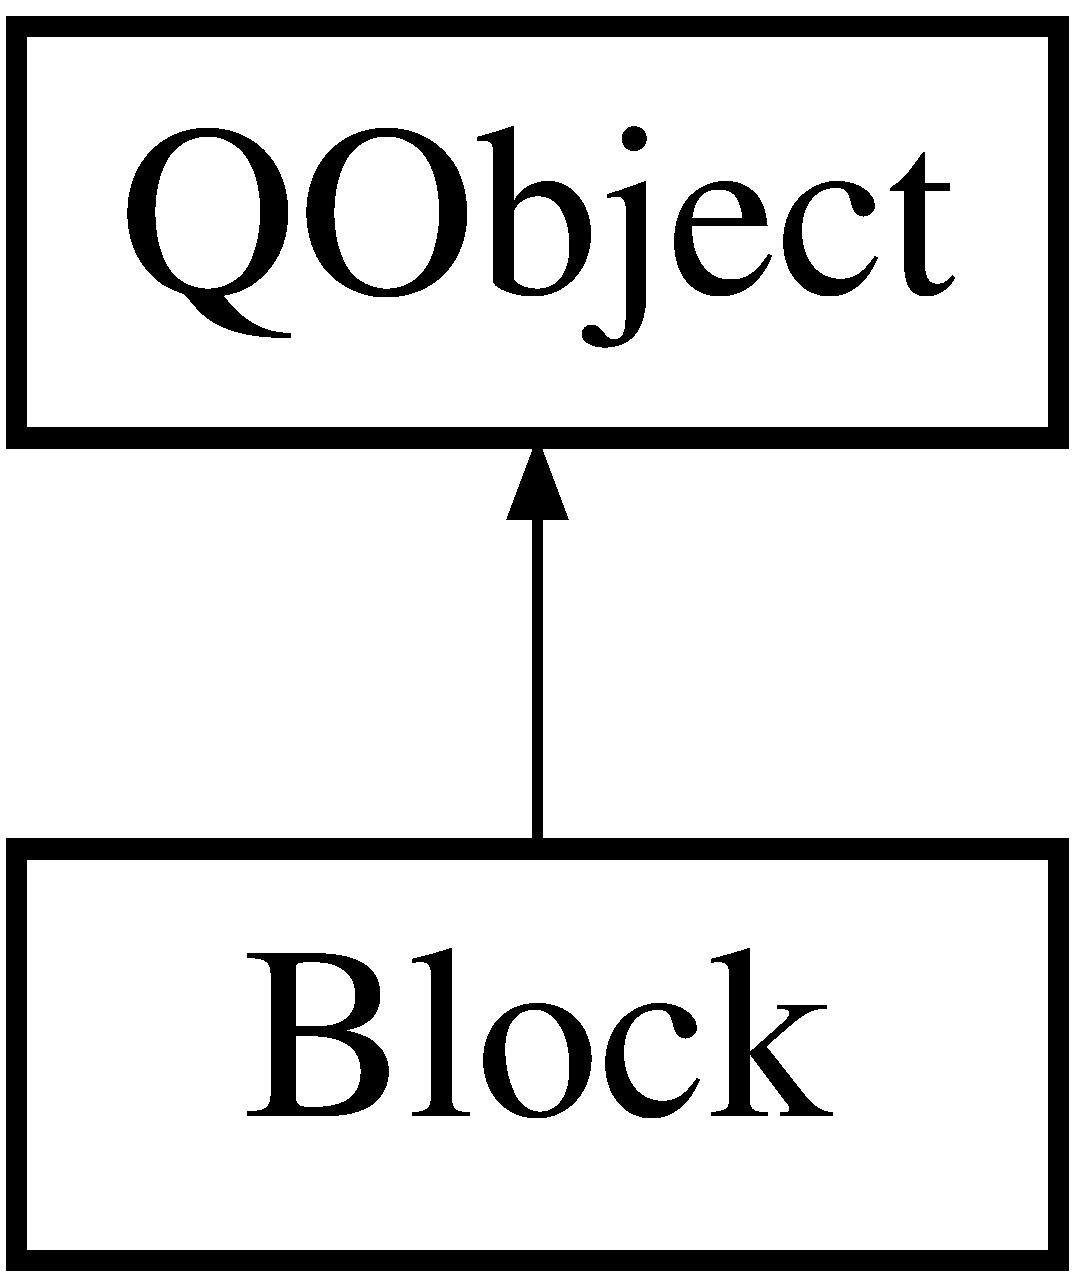
\includegraphics[height=2.000000cm]{class_block}
\end{center}
\end{figure}
\subsection*{Public Member Functions}
\begin{DoxyCompactItemize}
\item 
\hyperlink{class_block_acb9ba4b4221f41d888628a434052af6e}{Block} (b2\+World $\ast$world, Q\+Graphics\+Scene $\ast$level, b2\+Vec2 center, qreal m\+\_\+angle, qreal m\+\_\+length, qreal m\+\_\+width, b2\+Body\+Type type, qreal friction, Q\+String mode)
\begin{DoxyCompactList}\small\item\em \hyperlink{class_block_acb9ba4b4221f41d888628a434052af6e}{Block\+::\+Block}. \end{DoxyCompactList}\item 
void \hyperlink{class_block_a38b7625137a54cf57193c844163f9532}{draw\+Graphics} ()
\begin{DoxyCompactList}\small\item\em \hyperlink{class_block_a38b7625137a54cf57193c844163f9532}{Block\+::draw\+Graphics} connects the Box2\+D-\/\+Object to the Graphics after relocation. \end{DoxyCompactList}\end{DoxyCompactItemize}
\subsection*{Public Attributes}
\begin{DoxyCompactItemize}
\item 
qreal \hyperlink{class_block_a7ad40ed8c8d961b1ca2117835853a9c5}{length}
\item 
qreal \hyperlink{class_block_af7693d02f586bf02df6181995a66b768}{width}
\item 
qreal \hyperlink{class_block_ac19871a0cf41116b9585f34c3c21ec54}{angle}
\item 
b2\+Body $\ast$ \hyperlink{class_block_a5c9003f7f9cd6105465da994012085f8}{body}
\item 
Q\+Graphics\+Item $\ast$ \hyperlink{class_block_aab0690c05a4c1c8ee999647250b3e170}{graphics}
\end{DoxyCompactItemize}


\subsection{Detailed Description}


Definition at line 11 of file block.\+h.



\subsection{Constructor \& Destructor Documentation}
\index{Block@{Block}!Block@{Block}}
\index{Block@{Block}!Block@{Block}}
\subsubsection[{\texorpdfstring{Block(b2\+World $\ast$world, Q\+Graphics\+Scene $\ast$level, b2\+Vec2 center, qreal m\+\_\+angle, qreal m\+\_\+length, qreal m\+\_\+width, b2\+Body\+Type type, qreal friction, Q\+String mode)}{Block(b2World *world, QGraphicsScene *level, b2Vec2 center, qreal m_angle, qreal m_length, qreal m_width, b2BodyType type, qreal friction, QString mode)}}]{\setlength{\rightskip}{0pt plus 5cm}Block\+::\+Block (
\begin{DoxyParamCaption}
\item[{b2\+World $\ast$}]{world, }
\item[{Q\+Graphics\+Scene $\ast$}]{level, }
\item[{b2\+Vec2}]{center, }
\item[{qreal}]{m\+\_\+angle, }
\item[{qreal}]{m\+\_\+length, }
\item[{qreal}]{m\+\_\+width, }
\item[{b2\+Body\+Type}]{type, }
\item[{qreal}]{friction, }
\item[{Q\+String}]{mode}
\end{DoxyParamCaption}
)}\hypertarget{class_block_acb9ba4b4221f41d888628a434052af6e}{}\label{class_block_acb9ba4b4221f41d888628a434052af6e}


\hyperlink{class_block_acb9ba4b4221f41d888628a434052af6e}{Block\+::\+Block}. 


\begin{DoxyParams}{Parameters}
{\em world} & \+: Box2D world for physic engine \\
\hline
{\em level} & \+: Scene for the game \\
\hline
{\em center} & \+: is the centerposition of the block \\
\hline
{\em m\+\_\+angle} & angle for the block \\
\hline
{\em m\+\_\+length} & \+: length bock \\
\hline
{\em m\+\_\+width} & \+: width block \\
\hline
{\em type} & \+: Box2D type of the Bbock(if it\textquotesingle{}s static or dynamic) \\
\hline
{\em friction} & \+: friction for the \hyperlink{class_block}{Block} \\
\hline
{\em mode} & \+: is it a obstacle or a tool \\
\hline
\end{DoxyParams}


Definition at line 19 of file block.\+cpp.



\subsection{Member Function Documentation}
\index{Block@{Block}!draw\+Graphics@{draw\+Graphics}}
\index{draw\+Graphics@{draw\+Graphics}!Block@{Block}}
\subsubsection[{\texorpdfstring{draw\+Graphics()}{drawGraphics()}}]{\setlength{\rightskip}{0pt plus 5cm}void Block\+::draw\+Graphics (
\begin{DoxyParamCaption}
{}
\end{DoxyParamCaption}
)}\hypertarget{class_block_a38b7625137a54cf57193c844163f9532}{}\label{class_block_a38b7625137a54cf57193c844163f9532}


\hyperlink{class_block_a38b7625137a54cf57193c844163f9532}{Block\+::draw\+Graphics} connects the Box2\+D-\/\+Object to the Graphics after relocation. 



Definition at line 76 of file block.\+cpp.



\subsection{Member Data Documentation}
\index{Block@{Block}!angle@{angle}}
\index{angle@{angle}!Block@{Block}}
\subsubsection[{\texorpdfstring{angle}{angle}}]{\setlength{\rightskip}{0pt plus 5cm}qreal Block\+::angle}\hypertarget{class_block_ac19871a0cf41116b9585f34c3c21ec54}{}\label{class_block_ac19871a0cf41116b9585f34c3c21ec54}


Definition at line 21 of file block.\+h.

\index{Block@{Block}!body@{body}}
\index{body@{body}!Block@{Block}}
\subsubsection[{\texorpdfstring{body}{body}}]{\setlength{\rightskip}{0pt plus 5cm}b2\+Body$\ast$ Block\+::body}\hypertarget{class_block_a5c9003f7f9cd6105465da994012085f8}{}\label{class_block_a5c9003f7f9cd6105465da994012085f8}


Definition at line 22 of file block.\+h.

\index{Block@{Block}!graphics@{graphics}}
\index{graphics@{graphics}!Block@{Block}}
\subsubsection[{\texorpdfstring{graphics}{graphics}}]{\setlength{\rightskip}{0pt plus 5cm}Q\+Graphics\+Item$\ast$ Block\+::graphics}\hypertarget{class_block_aab0690c05a4c1c8ee999647250b3e170}{}\label{class_block_aab0690c05a4c1c8ee999647250b3e170}


Definition at line 23 of file block.\+h.

\index{Block@{Block}!length@{length}}
\index{length@{length}!Block@{Block}}
\subsubsection[{\texorpdfstring{length}{length}}]{\setlength{\rightskip}{0pt plus 5cm}qreal Block\+::length}\hypertarget{class_block_a7ad40ed8c8d961b1ca2117835853a9c5}{}\label{class_block_a7ad40ed8c8d961b1ca2117835853a9c5}


Definition at line 19 of file block.\+h.

\index{Block@{Block}!width@{width}}
\index{width@{width}!Block@{Block}}
\subsubsection[{\texorpdfstring{width}{width}}]{\setlength{\rightskip}{0pt plus 5cm}qreal Block\+::width}\hypertarget{class_block_af7693d02f586bf02df6181995a66b768}{}\label{class_block_af7693d02f586bf02df6181995a66b768}


Definition at line 20 of file block.\+h.



The documentation for this class was generated from the following files\+:\begin{DoxyCompactItemize}
\item 
C\+:/\+Users/\+Maximilian/\+Desktop/\+T\+U\+M/6.\+Semester/\+Grundkurs C++/\+Hauptprojekt/gruppe4\+\_\+hauptprojekt/gruppe4\+\_\+hauptprojekt/\+Game/\hyperlink{block_8h}{block.\+h}\item 
C\+:/\+Users/\+Maximilian/\+Desktop/\+T\+U\+M/6.\+Semester/\+Grundkurs C++/\+Hauptprojekt/gruppe4\+\_\+hauptprojekt/gruppe4\+\_\+hauptprojekt/\+Game/\hyperlink{block_8cpp}{block.\+cpp}\end{DoxyCompactItemize}

\hypertarget{class_circle}{}\section{Circle Class Reference}
\label{class_circle}\index{Circle@{Circle}}


{\ttfamily \#include $<$circle.\+h$>$}

Inheritance diagram for Circle\+:\begin{figure}[H]
\begin{center}
\leavevmode
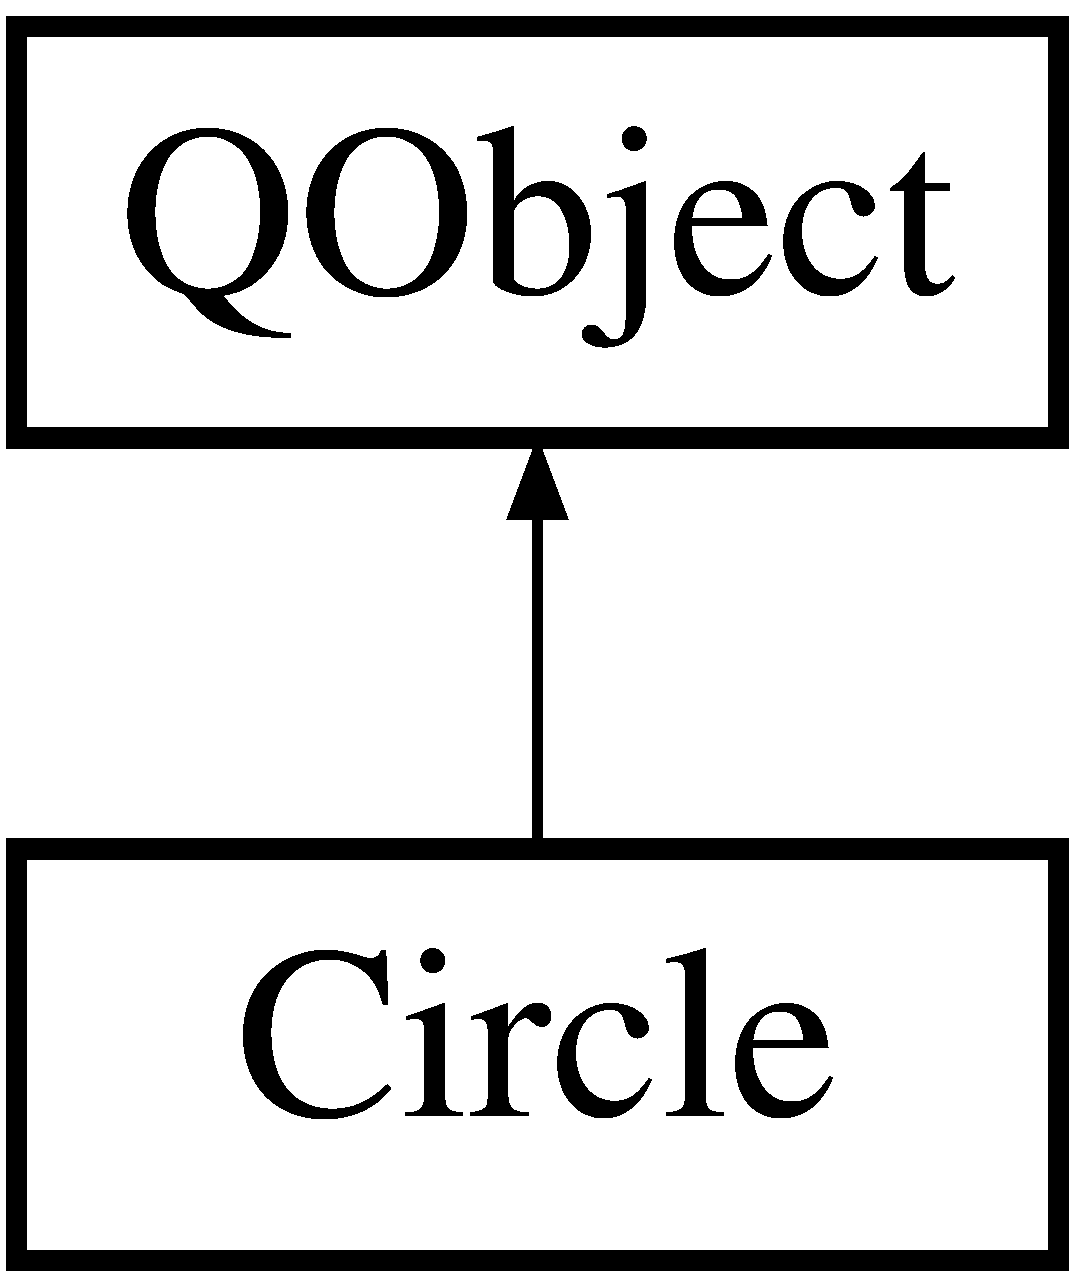
\includegraphics[height=2.000000cm]{class_circle}
\end{center}
\end{figure}
\subsection*{Public Member Functions}
\begin{DoxyCompactItemize}
\item 
\hyperlink{class_circle_af0186a5b261937e4902fa143968fb846}{Circle} (b2\+World $\ast$world, Q\+Graphics\+Scene $\ast$level, Q\+PointF position, qreal angle, b2\+Body\+Type type, b2\+Circle\+Shape \&circle, Q\+String mode)
\begin{DoxyCompactList}\small\item\em \hyperlink{class_circle_af0186a5b261937e4902fa143968fb846}{Circle\+::\+Circle}. \end{DoxyCompactList}\item 
void \hyperlink{class_circle_a3a3fea884c3f2865b00190d3c165e7cd}{create\+Circle} (b2\+World world, Q\+Graphics\+Scene levelscene, Q\+PointF pos, qreal angle, b2\+Body\+Type type, b2\+Circle\+Shape \&circle)
\item 
void \hyperlink{class_circle_a3a3f7166e7f629e44f9044b0e537eb22}{draw} ()
\begin{DoxyCompactList}\small\item\em \hyperlink{class_circle_a3a3f7166e7f629e44f9044b0e537eb22}{Circle\+::draw} connects the Graphics to the Box2\+D-\/\+Object. \end{DoxyCompactList}\item 
bool \hyperlink{class_circle_a71e6174daf2374f4c07361ba42c15276}{draw\+Ball1} ()
\begin{DoxyCompactList}\small\item\em \hyperlink{class_circle_a71e6174daf2374f4c07361ba42c15276}{Circle\+::draw\+Ball1} connects the Graphics to the Box2\+D-\/\+Object. \end{DoxyCompactList}\item 
void \hyperlink{class_circle_a62401396510855dbb2e3a2fb3444c90a}{draw\+Graphics} ()
\begin{DoxyCompactList}\small\item\em \hyperlink{class_circle_a62401396510855dbb2e3a2fb3444c90a}{Circle\+::draw\+Graphics} connects the Box2\+D-\/\+Object to the Graphics after relocation. \end{DoxyCompactList}\end{DoxyCompactItemize}
\subsection*{Public Attributes}
\begin{DoxyCompactItemize}
\item 
b2\+Body $\ast$ \hyperlink{class_circle_ac3736c952dbac0c813f6d98f29a3e34b}{body}
\begin{DoxyCompactList}\small\item\em Box2D Body of object. \end{DoxyCompactList}\item 
Q\+Graphics\+Item $\ast$ \hyperlink{class_circle_adcb606946696832caca242eafcc8322a}{graphics}
\begin{DoxyCompactList}\small\item\em graphic of object \end{DoxyCompactList}\end{DoxyCompactItemize}


\subsection{Constructor \& Destructor Documentation}
\index{Circle@{Circle}!Circle@{Circle}}
\index{Circle@{Circle}!Circle@{Circle}}
\subsubsection[{\texorpdfstring{Circle(b2\+World $\ast$world, Q\+Graphics\+Scene $\ast$level, Q\+Point\+F position, qreal angle, b2\+Body\+Type type, b2\+Circle\+Shape \&circle, Q\+String mode)}{Circle(b2World *world, QGraphicsScene *level, QPointF position, qreal angle, b2BodyType type, b2CircleShape &circle, QString mode)}}]{\setlength{\rightskip}{0pt plus 5cm}Circle\+::\+Circle (
\begin{DoxyParamCaption}
\item[{b2\+World $\ast$}]{world, }
\item[{Q\+Graphics\+Scene $\ast$}]{level, }
\item[{Q\+PointF}]{position, }
\item[{qreal}]{angle, }
\item[{b2\+Body\+Type}]{type, }
\item[{b2\+Circle\+Shape \&}]{circle, }
\item[{Q\+String}]{mode}
\end{DoxyParamCaption}
)}\hypertarget{class_circle_af0186a5b261937e4902fa143968fb846}{}\label{class_circle_af0186a5b261937e4902fa143968fb846}


\hyperlink{class_circle_af0186a5b261937e4902fa143968fb846}{Circle\+::\+Circle}. 


\begin{DoxyParams}{Parameters}
{\em world} & \+: Box2D world for physic engine \\
\hline
{\em level} & \+: Scene for the game \\
\hline
{\em position} & \+: left upper corner \\
\hline
{\em angle} & \+: angle for the circle \\
\hline
{\em type} & \+: Box2D type of the circle(if it\textquotesingle{}s static or dynamic) \\
\hline
{\em circle} & \+: Box2D knows that it is a circle \\
\hline
{\em mode} & \+: is it a obstacle or a tool \\
\hline
\end{DoxyParams}


\subsection{Member Function Documentation}
\index{Circle@{Circle}!create\+Circle@{create\+Circle}}
\index{create\+Circle@{create\+Circle}!Circle@{Circle}}
\subsubsection[{\texorpdfstring{create\+Circle(b2\+World world, Q\+Graphics\+Scene levelscene, Q\+Point\+F pos, qreal angle, b2\+Body\+Type type, b2\+Circle\+Shape \&circle)}{createCircle(b2World world, QGraphicsScene levelscene, QPointF pos, qreal angle, b2BodyType type, b2CircleShape &circle)}}]{\setlength{\rightskip}{0pt plus 5cm}void Circle\+::create\+Circle (
\begin{DoxyParamCaption}
\item[{b2\+World}]{world, }
\item[{Q\+Graphics\+Scene}]{levelscene, }
\item[{Q\+PointF}]{pos, }
\item[{qreal}]{angle, }
\item[{b2\+Body\+Type}]{type, }
\item[{b2\+Circle\+Shape \&}]{circle}
\end{DoxyParamCaption}
)}\hypertarget{class_circle_a3a3fea884c3f2865b00190d3c165e7cd}{}\label{class_circle_a3a3fea884c3f2865b00190d3c165e7cd}
\index{Circle@{Circle}!draw@{draw}}
\index{draw@{draw}!Circle@{Circle}}
\subsubsection[{\texorpdfstring{draw()}{draw()}}]{\setlength{\rightskip}{0pt plus 5cm}void Circle\+::draw (
\begin{DoxyParamCaption}
{}
\end{DoxyParamCaption}
)}\hypertarget{class_circle_a3a3f7166e7f629e44f9044b0e537eb22}{}\label{class_circle_a3a3f7166e7f629e44f9044b0e537eb22}


\hyperlink{class_circle_a3a3f7166e7f629e44f9044b0e537eb22}{Circle\+::draw} connects the Graphics to the Box2\+D-\/\+Object. 

\index{Circle@{Circle}!draw\+Ball1@{draw\+Ball1}}
\index{draw\+Ball1@{draw\+Ball1}!Circle@{Circle}}
\subsubsection[{\texorpdfstring{draw\+Ball1()}{drawBall1()}}]{\setlength{\rightskip}{0pt plus 5cm}bool Circle\+::draw\+Ball1 (
\begin{DoxyParamCaption}
{}
\end{DoxyParamCaption}
)}\hypertarget{class_circle_a71e6174daf2374f4c07361ba42c15276}{}\label{class_circle_a71e6174daf2374f4c07361ba42c15276}


\hyperlink{class_circle_a71e6174daf2374f4c07361ba42c15276}{Circle\+::draw\+Ball1} connects the Graphics to the Box2\+D-\/\+Object. 

\begin{DoxyReturn}{Returns}

\end{DoxyReturn}
\index{Circle@{Circle}!draw\+Graphics@{draw\+Graphics}}
\index{draw\+Graphics@{draw\+Graphics}!Circle@{Circle}}
\subsubsection[{\texorpdfstring{draw\+Graphics()}{drawGraphics()}}]{\setlength{\rightskip}{0pt plus 5cm}void Circle\+::draw\+Graphics (
\begin{DoxyParamCaption}
{}
\end{DoxyParamCaption}
)}\hypertarget{class_circle_a62401396510855dbb2e3a2fb3444c90a}{}\label{class_circle_a62401396510855dbb2e3a2fb3444c90a}


\hyperlink{class_circle_a62401396510855dbb2e3a2fb3444c90a}{Circle\+::draw\+Graphics} connects the Box2\+D-\/\+Object to the Graphics after relocation. 



\subsection{Member Data Documentation}
\index{Circle@{Circle}!body@{body}}
\index{body@{body}!Circle@{Circle}}
\subsubsection[{\texorpdfstring{body}{body}}]{\setlength{\rightskip}{0pt plus 5cm}b2\+Body$\ast$ Circle\+::body}\hypertarget{class_circle_ac3736c952dbac0c813f6d98f29a3e34b}{}\label{class_circle_ac3736c952dbac0c813f6d98f29a3e34b}


Box2D Body of object. 

\index{Circle@{Circle}!graphics@{graphics}}
\index{graphics@{graphics}!Circle@{Circle}}
\subsubsection[{\texorpdfstring{graphics}{graphics}}]{\setlength{\rightskip}{0pt plus 5cm}Q\+Graphics\+Item$\ast$ Circle\+::graphics}\hypertarget{class_circle_adcb606946696832caca242eafcc8322a}{}\label{class_circle_adcb606946696832caca242eafcc8322a}


graphic of object 



The documentation for this class was generated from the following files\+:\begin{DoxyCompactItemize}
\item 
C\+:/\+Users/\+Maximilian/\+Desktop/\+T\+U\+M/6.\+Semester/\+Grundkurs C++/\+Hauptprojekt/gruppe4\+\_\+hauptprojekt/gruppe4\+\_\+hauptprojekt/\+Game/\hyperlink{circle_8h}{circle.\+h}\item 
C\+:/\+Users/\+Maximilian/\+Desktop/\+T\+U\+M/6.\+Semester/\+Grundkurs C++/\+Hauptprojekt/gruppe4\+\_\+hauptprojekt/gruppe4\+\_\+hauptprojekt/\+Game/\hyperlink{circle_8cpp}{circle.\+cpp}\end{DoxyCompactItemize}

\hypertarget{class_g_u_i}{}\section{G\+UI Class Reference}
\label{class_g_u_i}\index{G\+UI@{G\+UI}}


The \hyperlink{class_g_u_i}{G\+UI} class.  




{\ttfamily \#include $<$gui.\+h$>$}

Inheritance diagram for G\+UI\+:\begin{figure}[H]
\begin{center}
\leavevmode
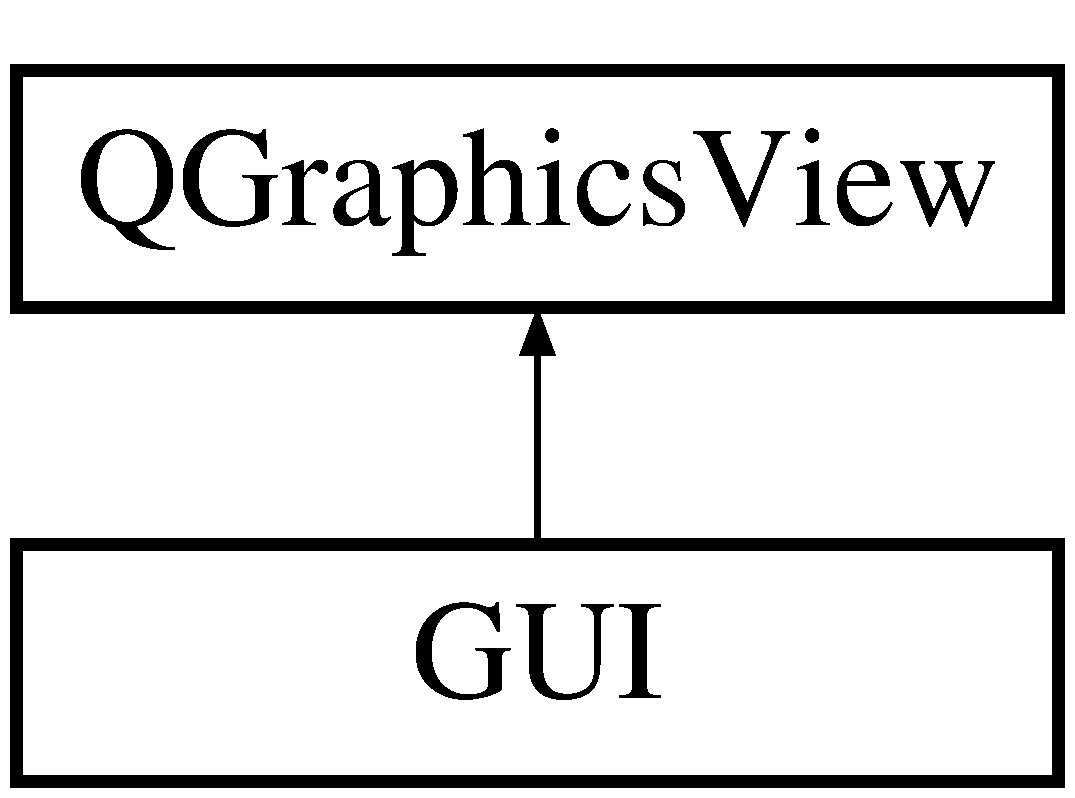
\includegraphics[height=2.000000cm]{class_g_u_i}
\end{center}
\end{figure}
\subsection*{Public Slots}
\begin{DoxyCompactItemize}
\item 
void \hyperlink{class_g_u_i_a9db2dc23fdc3aae57f9aaca530406365}{level\+Menu} ()
\begin{DoxyCompactList}\small\item\em \hyperlink{class_g_u_i_a9db2dc23fdc3aae57f9aaca530406365}{G\+U\+I\+::level\+Menu} opens the Levelmenu shows the Levels which can be selected(if they are enabled) opens the selected Level. \end{DoxyCompactList}\item 
void \hyperlink{class_g_u_i_a762402ea37d943ce0e94735895938117}{highscore} ()
\begin{DoxyCompactList}\small\item\em \hyperlink{class_g_u_i_a762402ea37d943ce0e94735895938117}{G\+U\+I\+::highscore} opens the Highscoretable and fill up the table for the level which are finished. \end{DoxyCompactList}\item 
void \hyperlink{class_g_u_i_aac5b92fad527c99c5aa84ed7fba970e3}{back} ()
\begin{DoxyCompactList}\small\item\em \hyperlink{class_g_u_i_aac5b92fad527c99c5aa84ed7fba970e3}{G\+U\+I\+::back}. \end{DoxyCompactList}\item 
void \hyperlink{class_g_u_i_a8de8197be4973e551cc0bc700f8112b3}{show\+Level1} ()
\begin{DoxyCompactList}\small\item\em \hyperlink{class_g_u_i_a8de8197be4973e551cc0bc700f8112b3}{G\+U\+I\+::show\+Level1} starts \hyperlink{class_level__1}{Level\+\_\+1} and hide gui. \end{DoxyCompactList}\item 
void \hyperlink{class_g_u_i_a5d12a36d8c4c0f9675054188ab6a4717}{show\+Level2} ()
\begin{DoxyCompactList}\small\item\em \hyperlink{class_g_u_i_a5d12a36d8c4c0f9675054188ab6a4717}{G\+U\+I\+::show\+Level2} starts \hyperlink{class_level__2}{Level\+\_\+2} and hide gui. \end{DoxyCompactList}\item 
void \hyperlink{class_g_u_i_ae93c49b9edadf4549bdac5caa3be5f2e}{show\+Level3} ()
\begin{DoxyCompactList}\small\item\em \hyperlink{class_g_u_i_ae93c49b9edadf4549bdac5caa3be5f2e}{G\+U\+I\+::show\+Level3} starts \hyperlink{class_level__3}{Level\+\_\+3} and hide gui. \end{DoxyCompactList}\item 
void \hyperlink{class_g_u_i_a40f7ec138fb724ef99b45aacb6c5d3d9}{show\+Level4} ()
\begin{DoxyCompactList}\small\item\em \hyperlink{class_g_u_i_a40f7ec138fb724ef99b45aacb6c5d3d9}{G\+U\+I\+::show\+Level4} starts \hyperlink{class_level__4}{Level\+\_\+4} and hide gui. \end{DoxyCompactList}\item 
void \hyperlink{class_g_u_i_afe5b1ca9bdc2b9565ce96ab6f2a01d6f}{show\+Guiagain} ()
\begin{DoxyCompactList}\small\item\em \hyperlink{class_g_u_i_afe5b1ca9bdc2b9565ce96ab6f2a01d6f}{G\+U\+I\+::show\+Guiagain} reopen \hyperlink{class_g_u_i}{G\+UI} after finish Level or close the level. \end{DoxyCompactList}\item 
void \hyperlink{class_g_u_i_a0cf2f8e739f52bd2e3c9c3605e50d875}{help} ()
\begin{DoxyCompactList}\small\item\em \hyperlink{class_g_u_i_a0cf2f8e739f52bd2e3c9c3605e50d875}{G\+U\+I\+::help} opens the Helpmenu. \end{DoxyCompactList}\item 
void \hyperlink{class_g_u_i_a41279e88f7b65e6aa5b5080dd0ce30fd}{box} ()
\begin{DoxyCompactList}\small\item\em \hyperlink{class_g_u_i_a41279e88f7b65e6aa5b5080dd0ce30fd}{G\+U\+I\+::box} box=rectangle helpmenu. \end{DoxyCompactList}\item 
void \hyperlink{class_g_u_i_a1c15a25fd741e4421ced2507a3f11596}{circle} ()
\begin{DoxyCompactList}\small\item\em \hyperlink{class_g_u_i_a1c15a25fd741e4421ced2507a3f11596}{G\+U\+I\+::circle} circle helpmenu. \end{DoxyCompactList}\item 
void \hyperlink{class_g_u_i_af5799c39952edf8560913cf4703ba493}{triangle} ()
\begin{DoxyCompactList}\small\item\em \hyperlink{class_g_u_i_af5799c39952edf8560913cf4703ba493}{G\+U\+I\+::triangle} triangle helpmenu. \end{DoxyCompactList}\item 
void \hyperlink{class_g_u_i_a8d3a63c2c3c112592bd7642da43b837b}{mute} ()
\begin{DoxyCompactList}\small\item\em \hyperlink{class_g_u_i_a8d3a63c2c3c112592bd7642da43b837b}{G\+U\+I\+::mute} enables and disables the backgroundsound. \end{DoxyCompactList}\item 
void \hyperlink{class_g_u_i_a4a69fe3a2286ff41bb870c4d387f5aff}{csnd} ()
\begin{DoxyCompactList}\small\item\em \hyperlink{class_g_u_i_a4a69fe3a2286ff41bb870c4d387f5aff}{G\+U\+I\+::csnd} paly sound if it is not muted. \end{DoxyCompactList}\end{DoxyCompactItemize}
\subsection*{Public Member Functions}
\begin{DoxyCompactItemize}
\item 
\hyperlink{class_g_u_i_a9524032d755910ed7cf4834ecf39dc42}{G\+UI} (Q\+Widget $\ast$parent=N\+U\+LL)
\begin{DoxyCompactList}\small\item\em \hyperlink{class_g_u_i_a9524032d755910ed7cf4834ecf39dc42}{G\+U\+I\+::\+G\+UI}. \end{DoxyCompactList}\item 
void \hyperlink{class_g_u_i_a329ff5d6462e5491f309830b4eee25f7}{display\+G\+UI} ()
\begin{DoxyCompactList}\small\item\em \hyperlink{class_g_u_i_a329ff5d6462e5491f309830b4eee25f7}{G\+U\+I\+::display\+G\+UI} opens the Startmenu creates the needed Buttons and connects them. \end{DoxyCompactList}\item 
void \hyperlink{class_g_u_i_acf0edc3e3efe914e04e0dcb416cf29f1}{check\+Level} ()
\begin{DoxyCompactList}\small\item\em \hyperlink{class_g_u_i_acf0edc3e3efe914e04e0dcb416cf29f1}{G\+U\+I\+::check\+Level} read out level.\+txt and fill the content in levelenab. \end{DoxyCompactList}\end{DoxyCompactItemize}
\subsection*{Public Attributes}
\begin{DoxyCompactItemize}
\item 
Q\+Graphics\+Scene $\ast$ \hyperlink{class_g_u_i_a52022e4c94d0e0378ed17b2348ed02db}{scene}
\begin{DoxyCompactList}\small\item\em Scene for \hyperlink{class_g_u_i}{G\+UI}. \end{DoxyCompactList}\item 
\hyperlink{classpic_button}{pic\+Button} $\ast$ \hyperlink{class_g_u_i_a7ad3ce9d9430e60063a1df9c21c21b41}{mutepic\+Button}
\begin{DoxyCompactList}\small\item\em Mutepicbutton for Sound. \end{DoxyCompactList}\item 
bool \hyperlink{class_g_u_i_ab44acd2396d4e2cb0cd8d285a58746d1}{ismute} = false
\begin{DoxyCompactList}\small\item\em Check if Sound is on or off. \end{DoxyCompactList}\end{DoxyCompactItemize}


\subsection{Detailed Description}
The \hyperlink{class_g_u_i}{G\+UI} class. 

\subsection{Constructor \& Destructor Documentation}
\index{G\+UI@{G\+UI}!G\+UI@{G\+UI}}
\index{G\+UI@{G\+UI}!G\+UI@{G\+UI}}
\subsubsection[{\texorpdfstring{G\+U\+I(\+Q\+Widget $\ast$parent=\+N\+U\+L\+L)}{GUI(QWidget *parent=NULL)}}]{\setlength{\rightskip}{0pt plus 5cm}G\+U\+I\+::\+G\+UI (
\begin{DoxyParamCaption}
\item[{Q\+Widget $\ast$}]{parent = {\ttfamily NULL}}
\end{DoxyParamCaption}
)}\hypertarget{class_g_u_i_a9524032d755910ed7cf4834ecf39dc42}{}\label{class_g_u_i_a9524032d755910ed7cf4834ecf39dc42}


\hyperlink{class_g_u_i_a9524032d755910ed7cf4834ecf39dc42}{G\+U\+I\+::\+G\+UI}. 


\begin{DoxyParams}{Parameters}
{\em parent} & Create Q\+Graphics\+View and enter scene \\
\hline
\end{DoxyParams}
Screen setup. No scroll bar available

Set Application-\/\+Name

Scene setup

ismute false by default

Sound 

\subsection{Member Function Documentation}
\index{G\+UI@{G\+UI}!back@{back}}
\index{back@{back}!G\+UI@{G\+UI}}
\subsubsection[{\texorpdfstring{back}{back}}]{\setlength{\rightskip}{0pt plus 5cm}void G\+U\+I\+::back (
\begin{DoxyParamCaption}
{}
\end{DoxyParamCaption}
)\hspace{0.3cm}{\ttfamily [slot]}}\hypertarget{class_g_u_i_aac5b92fad527c99c5aa84ed7fba970e3}{}\label{class_g_u_i_aac5b92fad527c99c5aa84ed7fba970e3}


\hyperlink{class_g_u_i_aac5b92fad527c99c5aa84ed7fba970e3}{G\+U\+I\+::back}. 

\index{G\+UI@{G\+UI}!box@{box}}
\index{box@{box}!G\+UI@{G\+UI}}
\subsubsection[{\texorpdfstring{box}{box}}]{\setlength{\rightskip}{0pt plus 5cm}void G\+U\+I\+::box (
\begin{DoxyParamCaption}
{}
\end{DoxyParamCaption}
)\hspace{0.3cm}{\ttfamily [slot]}}\hypertarget{class_g_u_i_a41279e88f7b65e6aa5b5080dd0ce30fd}{}\label{class_g_u_i_a41279e88f7b65e6aa5b5080dd0ce30fd}


\hyperlink{class_g_u_i_a41279e88f7b65e6aa5b5080dd0ce30fd}{G\+U\+I\+::box} box=rectangle helpmenu. 

create title text \index{G\+UI@{G\+UI}!check\+Level@{check\+Level}}
\index{check\+Level@{check\+Level}!G\+UI@{G\+UI}}
\subsubsection[{\texorpdfstring{check\+Level()}{checkLevel()}}]{\setlength{\rightskip}{0pt plus 5cm}void G\+U\+I\+::check\+Level (
\begin{DoxyParamCaption}
{}
\end{DoxyParamCaption}
)}\hypertarget{class_g_u_i_acf0edc3e3efe914e04e0dcb416cf29f1}{}\label{class_g_u_i_acf0edc3e3efe914e04e0dcb416cf29f1}


\hyperlink{class_g_u_i_acf0edc3e3efe914e04e0dcb416cf29f1}{G\+U\+I\+::check\+Level} read out level.\+txt and fill the content in levelenab. 

\index{G\+UI@{G\+UI}!circle@{circle}}
\index{circle@{circle}!G\+UI@{G\+UI}}
\subsubsection[{\texorpdfstring{circle}{circle}}]{\setlength{\rightskip}{0pt plus 5cm}void G\+U\+I\+::circle (
\begin{DoxyParamCaption}
{}
\end{DoxyParamCaption}
)\hspace{0.3cm}{\ttfamily [slot]}}\hypertarget{class_g_u_i_a1c15a25fd741e4421ced2507a3f11596}{}\label{class_g_u_i_a1c15a25fd741e4421ced2507a3f11596}


\hyperlink{class_g_u_i_a1c15a25fd741e4421ced2507a3f11596}{G\+U\+I\+::circle} circle helpmenu. 

create title text \index{G\+UI@{G\+UI}!csnd@{csnd}}
\index{csnd@{csnd}!G\+UI@{G\+UI}}
\subsubsection[{\texorpdfstring{csnd}{csnd}}]{\setlength{\rightskip}{0pt plus 5cm}void G\+U\+I\+::csnd (
\begin{DoxyParamCaption}
{}
\end{DoxyParamCaption}
)\hspace{0.3cm}{\ttfamily [slot]}}\hypertarget{class_g_u_i_a4a69fe3a2286ff41bb870c4d387f5aff}{}\label{class_g_u_i_a4a69fe3a2286ff41bb870c4d387f5aff}


\hyperlink{class_g_u_i_a4a69fe3a2286ff41bb870c4d387f5aff}{G\+U\+I\+::csnd} paly sound if it is not muted. 

\index{G\+UI@{G\+UI}!display\+G\+UI@{display\+G\+UI}}
\index{display\+G\+UI@{display\+G\+UI}!G\+UI@{G\+UI}}
\subsubsection[{\texorpdfstring{display\+G\+U\+I()}{displayGUI()}}]{\setlength{\rightskip}{0pt plus 5cm}void G\+U\+I\+::display\+G\+UI (
\begin{DoxyParamCaption}
{}
\end{DoxyParamCaption}
)}\hypertarget{class_g_u_i_a329ff5d6462e5491f309830b4eee25f7}{}\label{class_g_u_i_a329ff5d6462e5491f309830b4eee25f7}


\hyperlink{class_g_u_i_a329ff5d6462e5491f309830b4eee25f7}{G\+U\+I\+::display\+G\+UI} opens the Startmenu creates the needed Buttons and connects them. 

create title text

create level menu button

create highscore button

create help button

create quit button

create sound button\index{G\+UI@{G\+UI}!help@{help}}
\index{help@{help}!G\+UI@{G\+UI}}
\subsubsection[{\texorpdfstring{help}{help}}]{\setlength{\rightskip}{0pt plus 5cm}void G\+U\+I\+::help (
\begin{DoxyParamCaption}
{}
\end{DoxyParamCaption}
)\hspace{0.3cm}{\ttfamily [slot]}}\hypertarget{class_g_u_i_a0cf2f8e739f52bd2e3c9c3605e50d875}{}\label{class_g_u_i_a0cf2f8e739f52bd2e3c9c3605e50d875}


\hyperlink{class_g_u_i_a0cf2f8e739f52bd2e3c9c3605e50d875}{G\+U\+I\+::help} opens the Helpmenu. 

create title text \index{G\+UI@{G\+UI}!highscore@{highscore}}
\index{highscore@{highscore}!G\+UI@{G\+UI}}
\subsubsection[{\texorpdfstring{highscore}{highscore}}]{\setlength{\rightskip}{0pt plus 5cm}void G\+U\+I\+::highscore (
\begin{DoxyParamCaption}
{}
\end{DoxyParamCaption}
)\hspace{0.3cm}{\ttfamily [slot]}}\hypertarget{class_g_u_i_a762402ea37d943ce0e94735895938117}{}\label{class_g_u_i_a762402ea37d943ce0e94735895938117}


\hyperlink{class_g_u_i_a762402ea37d943ce0e94735895938117}{G\+U\+I\+::highscore} opens the Highscoretable and fill up the table for the level which are finished. 

create title text \index{G\+UI@{G\+UI}!level\+Menu@{level\+Menu}}
\index{level\+Menu@{level\+Menu}!G\+UI@{G\+UI}}
\subsubsection[{\texorpdfstring{level\+Menu}{levelMenu}}]{\setlength{\rightskip}{0pt plus 5cm}void G\+U\+I\+::level\+Menu (
\begin{DoxyParamCaption}
{}
\end{DoxyParamCaption}
)\hspace{0.3cm}{\ttfamily [slot]}}\hypertarget{class_g_u_i_a9db2dc23fdc3aae57f9aaca530406365}{}\label{class_g_u_i_a9db2dc23fdc3aae57f9aaca530406365}


\hyperlink{class_g_u_i_a9db2dc23fdc3aae57f9aaca530406365}{G\+U\+I\+::level\+Menu} opens the Levelmenu shows the Levels which can be selected(if they are enabled) opens the selected Level. 

create level menu button \index{G\+UI@{G\+UI}!mute@{mute}}
\index{mute@{mute}!G\+UI@{G\+UI}}
\subsubsection[{\texorpdfstring{mute}{mute}}]{\setlength{\rightskip}{0pt plus 5cm}void G\+U\+I\+::mute (
\begin{DoxyParamCaption}
{}
\end{DoxyParamCaption}
)\hspace{0.3cm}{\ttfamily [slot]}}\hypertarget{class_g_u_i_a8d3a63c2c3c112592bd7642da43b837b}{}\label{class_g_u_i_a8d3a63c2c3c112592bd7642da43b837b}


\hyperlink{class_g_u_i_a8d3a63c2c3c112592bd7642da43b837b}{G\+U\+I\+::mute} enables and disables the backgroundsound. 

\index{G\+UI@{G\+UI}!show\+Guiagain@{show\+Guiagain}}
\index{show\+Guiagain@{show\+Guiagain}!G\+UI@{G\+UI}}
\subsubsection[{\texorpdfstring{show\+Guiagain}{showGuiagain}}]{\setlength{\rightskip}{0pt plus 5cm}void G\+U\+I\+::show\+Guiagain (
\begin{DoxyParamCaption}
{}
\end{DoxyParamCaption}
)\hspace{0.3cm}{\ttfamily [slot]}}\hypertarget{class_g_u_i_afe5b1ca9bdc2b9565ce96ab6f2a01d6f}{}\label{class_g_u_i_afe5b1ca9bdc2b9565ce96ab6f2a01d6f}


\hyperlink{class_g_u_i_afe5b1ca9bdc2b9565ce96ab6f2a01d6f}{G\+U\+I\+::show\+Guiagain} reopen \hyperlink{class_g_u_i}{G\+UI} after finish Level or close the level. 

\index{G\+UI@{G\+UI}!show\+Level1@{show\+Level1}}
\index{show\+Level1@{show\+Level1}!G\+UI@{G\+UI}}
\subsubsection[{\texorpdfstring{show\+Level1}{showLevel1}}]{\setlength{\rightskip}{0pt plus 5cm}void G\+U\+I\+::show\+Level1 (
\begin{DoxyParamCaption}
{}
\end{DoxyParamCaption}
)\hspace{0.3cm}{\ttfamily [slot]}}\hypertarget{class_g_u_i_a8de8197be4973e551cc0bc700f8112b3}{}\label{class_g_u_i_a8de8197be4973e551cc0bc700f8112b3}


\hyperlink{class_g_u_i_a8de8197be4973e551cc0bc700f8112b3}{G\+U\+I\+::show\+Level1} starts \hyperlink{class_level__1}{Level\+\_\+1} and hide gui. 

\index{G\+UI@{G\+UI}!show\+Level2@{show\+Level2}}
\index{show\+Level2@{show\+Level2}!G\+UI@{G\+UI}}
\subsubsection[{\texorpdfstring{show\+Level2}{showLevel2}}]{\setlength{\rightskip}{0pt plus 5cm}void G\+U\+I\+::show\+Level2 (
\begin{DoxyParamCaption}
{}
\end{DoxyParamCaption}
)\hspace{0.3cm}{\ttfamily [slot]}}\hypertarget{class_g_u_i_a5d12a36d8c4c0f9675054188ab6a4717}{}\label{class_g_u_i_a5d12a36d8c4c0f9675054188ab6a4717}


\hyperlink{class_g_u_i_a5d12a36d8c4c0f9675054188ab6a4717}{G\+U\+I\+::show\+Level2} starts \hyperlink{class_level__2}{Level\+\_\+2} and hide gui. 

\index{G\+UI@{G\+UI}!show\+Level3@{show\+Level3}}
\index{show\+Level3@{show\+Level3}!G\+UI@{G\+UI}}
\subsubsection[{\texorpdfstring{show\+Level3}{showLevel3}}]{\setlength{\rightskip}{0pt plus 5cm}void G\+U\+I\+::show\+Level3 (
\begin{DoxyParamCaption}
{}
\end{DoxyParamCaption}
)\hspace{0.3cm}{\ttfamily [slot]}}\hypertarget{class_g_u_i_ae93c49b9edadf4549bdac5caa3be5f2e}{}\label{class_g_u_i_ae93c49b9edadf4549bdac5caa3be5f2e}


\hyperlink{class_g_u_i_ae93c49b9edadf4549bdac5caa3be5f2e}{G\+U\+I\+::show\+Level3} starts \hyperlink{class_level__3}{Level\+\_\+3} and hide gui. 

\index{G\+UI@{G\+UI}!show\+Level4@{show\+Level4}}
\index{show\+Level4@{show\+Level4}!G\+UI@{G\+UI}}
\subsubsection[{\texorpdfstring{show\+Level4}{showLevel4}}]{\setlength{\rightskip}{0pt plus 5cm}void G\+U\+I\+::show\+Level4 (
\begin{DoxyParamCaption}
{}
\end{DoxyParamCaption}
)\hspace{0.3cm}{\ttfamily [slot]}}\hypertarget{class_g_u_i_a40f7ec138fb724ef99b45aacb6c5d3d9}{}\label{class_g_u_i_a40f7ec138fb724ef99b45aacb6c5d3d9}


\hyperlink{class_g_u_i_a40f7ec138fb724ef99b45aacb6c5d3d9}{G\+U\+I\+::show\+Level4} starts \hyperlink{class_level__4}{Level\+\_\+4} and hide gui. 

\index{G\+UI@{G\+UI}!triangle@{triangle}}
\index{triangle@{triangle}!G\+UI@{G\+UI}}
\subsubsection[{\texorpdfstring{triangle}{triangle}}]{\setlength{\rightskip}{0pt plus 5cm}void G\+U\+I\+::triangle (
\begin{DoxyParamCaption}
{}
\end{DoxyParamCaption}
)\hspace{0.3cm}{\ttfamily [slot]}}\hypertarget{class_g_u_i_af5799c39952edf8560913cf4703ba493}{}\label{class_g_u_i_af5799c39952edf8560913cf4703ba493}


\hyperlink{class_g_u_i_af5799c39952edf8560913cf4703ba493}{G\+U\+I\+::triangle} triangle helpmenu. 

create title text 

\subsection{Member Data Documentation}
\index{G\+UI@{G\+UI}!ismute@{ismute}}
\index{ismute@{ismute}!G\+UI@{G\+UI}}
\subsubsection[{\texorpdfstring{ismute}{ismute}}]{\setlength{\rightskip}{0pt plus 5cm}bool G\+U\+I\+::ismute = false}\hypertarget{class_g_u_i_ab44acd2396d4e2cb0cd8d285a58746d1}{}\label{class_g_u_i_ab44acd2396d4e2cb0cd8d285a58746d1}


Check if Sound is on or off. 

\index{G\+UI@{G\+UI}!mutepic\+Button@{mutepic\+Button}}
\index{mutepic\+Button@{mutepic\+Button}!G\+UI@{G\+UI}}
\subsubsection[{\texorpdfstring{mutepic\+Button}{mutepicButton}}]{\setlength{\rightskip}{0pt plus 5cm}{\bf pic\+Button}$\ast$ G\+U\+I\+::mutepic\+Button}\hypertarget{class_g_u_i_a7ad3ce9d9430e60063a1df9c21c21b41}{}\label{class_g_u_i_a7ad3ce9d9430e60063a1df9c21c21b41}


Mutepicbutton for Sound. 

\index{G\+UI@{G\+UI}!scene@{scene}}
\index{scene@{scene}!G\+UI@{G\+UI}}
\subsubsection[{\texorpdfstring{scene}{scene}}]{\setlength{\rightskip}{0pt plus 5cm}Q\+Graphics\+Scene$\ast$ G\+U\+I\+::scene}\hypertarget{class_g_u_i_a52022e4c94d0e0378ed17b2348ed02db}{}\label{class_g_u_i_a52022e4c94d0e0378ed17b2348ed02db}


Scene for \hyperlink{class_g_u_i}{G\+UI}. 



The documentation for this class was generated from the following files\+:\begin{DoxyCompactItemize}
\item 
C\+:/\+Users/\+Maximilian/\+Desktop/\+T\+U\+M/6.\+Semester/\+Grundkurs C++/\+Hauptprojekt/gruppe4\+\_\+hauptprojekt/gruppe4\+\_\+hauptprojekt/\+Game/\hyperlink{gui_8h}{gui.\+h}\item 
C\+:/\+Users/\+Maximilian/\+Desktop/\+T\+U\+M/6.\+Semester/\+Grundkurs C++/\+Hauptprojekt/gruppe4\+\_\+hauptprojekt/gruppe4\+\_\+hauptprojekt/\+Game/\hyperlink{gui_8cpp}{gui.\+cpp}\end{DoxyCompactItemize}

\hypertarget{class_level__1}{}\section{Level\+\_\+1 Class Reference}
\label{class_level__1}\index{Level\+\_\+1@{Level\+\_\+1}}


{\ttfamily \#include $<$level\+\_\+1.\+h$>$}

Inheritance diagram for Level\+\_\+1\+:\begin{figure}[H]
\begin{center}
\leavevmode
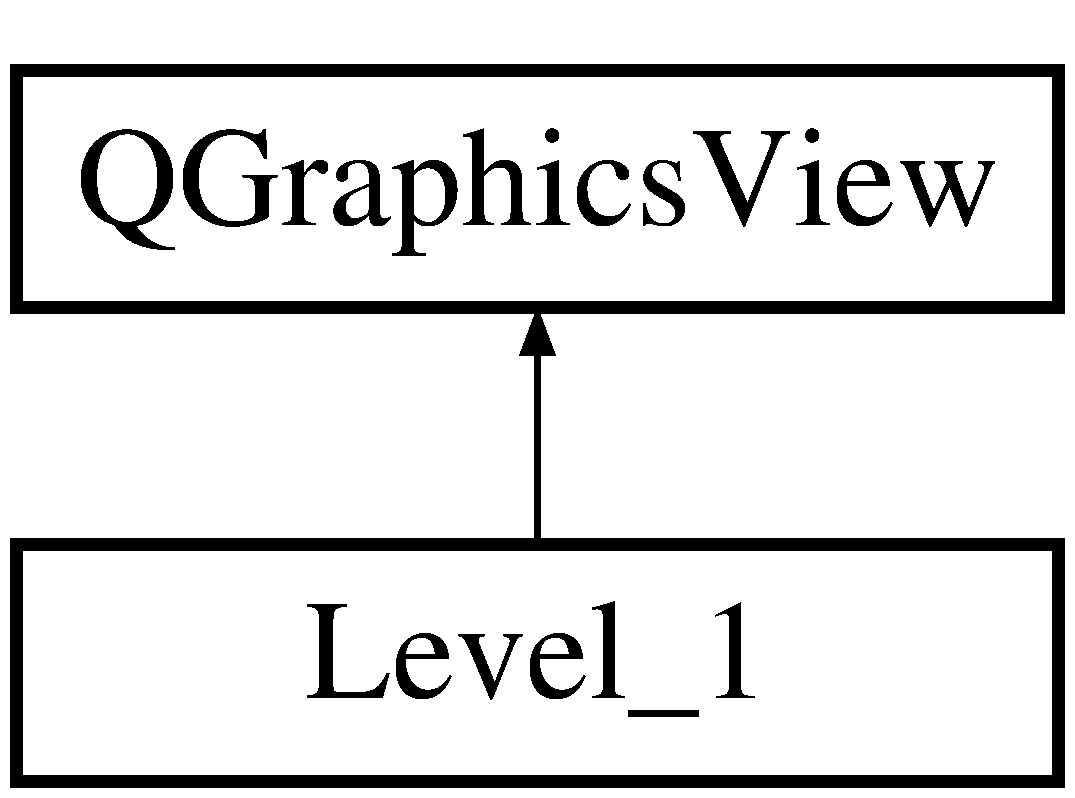
\includegraphics[height=2.000000cm]{class_level__1}
\end{center}
\end{figure}
\subsection*{Public Slots}
\begin{DoxyCompactItemize}
\item 
void \hyperlink{class_level__1_ac400cc08cdf56f15e640c454d5f67196}{update} ()
\begin{DoxyCompactList}\small\item\em \hyperlink{class_level__1_ac400cc08cdf56f15e640c454d5f67196}{Level\+\_\+1\+::update} update function for moveable objects like our ball -\/ sets the graphics of the ball to the position of the box2D body. \end{DoxyCompactList}\item 
void \hyperlink{class_level__1_ae190005d1364005c16bb9cb01cd641d8}{start\+Level} ()
\begin{DoxyCompactList}\small\item\em \hyperlink{class_level__1_ae190005d1364005c16bb9cb01cd641d8}{Level\+\_\+1\+::start\+Level} Set the flag of the Q\+Graphics\+Item, after start was clicked. draw the graphics if the body was moved before start was clicked. \end{DoxyCompactList}\item 
void \hyperlink{class_level__1_a00de500ddbbbc348b863cf0f43f68ca1}{pause\+Level} ()
\begin{DoxyCompactList}\small\item\em \hyperlink{class_level__1_a00de500ddbbbc348b863cf0f43f68ca1}{Level\+\_\+1\+::pause\+Level} pauses game when button pause is clicked. \end{DoxyCompactList}\item 
void \hyperlink{class_level__1_a1bd68401a5c8df24771bfc28c694a0a4}{resume\+Level} ()
\begin{DoxyCompactList}\small\item\em \hyperlink{class_level__1_a1bd68401a5c8df24771bfc28c694a0a4}{Level\+\_\+1\+::resume\+Level} resumes game when button resume is clicked. \end{DoxyCompactList}\item 
void \hyperlink{class_level__1_adf86596e7fa8f4c7ebd29517cfb0d8b2}{add\+Rectangle} ()
\begin{DoxyCompactList}\small\item\em \hyperlink{class_level__1_adf86596e7fa8f4c7ebd29517cfb0d8b2}{Level\+\_\+1\+::add\+Rectangle} Create new rectangle and count the rectangle items. limited to number. \end{DoxyCompactList}\item 
void \hyperlink{class_level__1_a1dee4bbb2dffb25a324fded0e50e47cb}{add\+Circle} ()
\begin{DoxyCompactList}\small\item\em \hyperlink{class_level__1_a1dee4bbb2dffb25a324fded0e50e47cb}{Level\+\_\+1\+::add\+Circle} create new circle and count the circle items. limited to number. \end{DoxyCompactList}\item 
void \hyperlink{class_level__1_ac8dc0a81168620b78aea1fb39b449a7f}{reset} ()
\begin{DoxyCompactList}\small\item\em \hyperlink{class_level__1_ac8dc0a81168620b78aea1fb39b449a7f}{Level\+\_\+1\+::reset} Clear scene and load Level again. \end{DoxyCompactList}\item 
void \hyperlink{class_level__1_af17fff3abb47ed9759df00d40a37dcc9}{close\+Level} ()
\begin{DoxyCompactList}\small\item\em \hyperlink{class_level__1_af17fff3abb47ed9759df00d40a37dcc9}{Level\+\_\+1\+::close\+Level} if Q\+Graphics\+View is closed emit Signal. \end{DoxyCompactList}\item 
void \hyperlink{class_level__1_ac214f4650ce42e7fa28834a6a95c4986}{rotate\+Left} ()
\begin{DoxyCompactList}\small\item\em \hyperlink{class_level__1_ac214f4650ce42e7fa28834a6a95c4986}{Level\+\_\+1\+::rotate\+Left} possibility to rotate objects to the left. \end{DoxyCompactList}\item 
void \hyperlink{class_level__1_ac28b3fe439dd840e3a37ab8132f94782}{rotate\+Right} ()
\begin{DoxyCompactList}\small\item\em \hyperlink{class_level__1_ac28b3fe439dd840e3a37ab8132f94782}{Level\+\_\+1\+::rotate\+Right} possibility to rotate right. \end{DoxyCompactList}\item 
void \hyperlink{class_level__1_a9614a513f31c3a76a892af6d88821e7b}{get\+Time} ()
\begin{DoxyCompactList}\small\item\em \hyperlink{class_level__1_a9614a513f31c3a76a892af6d88821e7b}{Level\+\_\+1\+::get\+Time} Stop time and convert it to ms. \end{DoxyCompactList}\item 
void \hyperlink{class_level__1_a2ac0de1428934d30d1b62d2c01aba04f}{highscore\+Counter} ()
\begin{DoxyCompactList}\small\item\em \hyperlink{class_level__1_a2ac0de1428934d30d1b62d2c01aba04f}{Level\+\_\+1\+::highscore\+Counter} Calculate the highscore. \end{DoxyCompactList}\end{DoxyCompactItemize}
\subsection*{Signals}
\begin{DoxyCompactItemize}
\item 
void \hyperlink{class_level__1_a8910744606161583b969261fa1f0de4a}{levelcompleted} ()
\end{DoxyCompactItemize}
\subsection*{Public Member Functions}
\begin{DoxyCompactItemize}
\item 
\hyperlink{class_level__1_a31b713ea291774e5eac40e1f1ab7faad}{Level\+\_\+1} ()
\begin{DoxyCompactList}\small\item\em \hyperlink{class_level__1_a31b713ea291774e5eac40e1f1ab7faad}{Level\+\_\+1\+::\+Level\+\_\+1}. \end{DoxyCompactList}\end{DoxyCompactItemize}
\subsection*{Public Attributes}
\begin{DoxyCompactItemize}
\item 
std\+::vector$<$ \hyperlink{class_block}{Block} $\ast$ $>$ \hyperlink{class_level__1_a18c333a1770f5ff2d46253a2acce5c25}{vectb}
\item 
std\+::vector$<$ \hyperlink{class_triangle}{Triangle} $\ast$ $>$ \hyperlink{class_level__1_a105889f16d0a0c733256b6f1be02d156}{vectt}
\end{DoxyCompactItemize}


\subsection{Detailed Description}


Definition at line 28 of file level\+\_\+1.\+h.



\subsection{Constructor \& Destructor Documentation}
\index{Level\+\_\+1@{Level\+\_\+1}!Level\+\_\+1@{Level\+\_\+1}}
\index{Level\+\_\+1@{Level\+\_\+1}!Level\+\_\+1@{Level\+\_\+1}}
\subsubsection[{\texorpdfstring{Level\+\_\+1()}{Level_1()}}]{\setlength{\rightskip}{0pt plus 5cm}Level\+\_\+1\+::\+Level\+\_\+1 (
\begin{DoxyParamCaption}
{}
\end{DoxyParamCaption}
)}\hypertarget{class_level__1_a31b713ea291774e5eac40e1f1ab7faad}{}\label{class_level__1_a31b713ea291774e5eac40e1f1ab7faad}


\hyperlink{class_level__1_a31b713ea291774e5eac40e1f1ab7faad}{Level\+\_\+1\+::\+Level\+\_\+1}. 


\begin{DoxyParams}{Parameters}
{\em parent} & Initialize Level1 -\/ Screen/\+Scene Setup... \\
\hline
\end{DoxyParams}
Set Application-\/\+Name 

Definition at line 21 of file level\+\_\+1.\+cpp.



\subsection{Member Function Documentation}
\index{Level\+\_\+1@{Level\+\_\+1}!add\+Circle@{add\+Circle}}
\index{add\+Circle@{add\+Circle}!Level\+\_\+1@{Level\+\_\+1}}
\subsubsection[{\texorpdfstring{add\+Circle}{addCircle}}]{\setlength{\rightskip}{0pt plus 5cm}void Level\+\_\+1\+::add\+Circle (
\begin{DoxyParamCaption}
{}
\end{DoxyParamCaption}
)\hspace{0.3cm}{\ttfamily [slot]}}\hypertarget{class_level__1_a1dee4bbb2dffb25a324fded0e50e47cb}{}\label{class_level__1_a1dee4bbb2dffb25a324fded0e50e47cb}


\hyperlink{class_level__1_a1dee4bbb2dffb25a324fded0e50e47cb}{Level\+\_\+1\+::add\+Circle} create new circle and count the circle items. limited to number. 



Definition at line 260 of file level\+\_\+1.\+cpp.

\index{Level\+\_\+1@{Level\+\_\+1}!add\+Rectangle@{add\+Rectangle}}
\index{add\+Rectangle@{add\+Rectangle}!Level\+\_\+1@{Level\+\_\+1}}
\subsubsection[{\texorpdfstring{add\+Rectangle}{addRectangle}}]{\setlength{\rightskip}{0pt plus 5cm}void Level\+\_\+1\+::add\+Rectangle (
\begin{DoxyParamCaption}
{}
\end{DoxyParamCaption}
)\hspace{0.3cm}{\ttfamily [slot]}}\hypertarget{class_level__1_adf86596e7fa8f4c7ebd29517cfb0d8b2}{}\label{class_level__1_adf86596e7fa8f4c7ebd29517cfb0d8b2}


\hyperlink{class_level__1_adf86596e7fa8f4c7ebd29517cfb0d8b2}{Level\+\_\+1\+::add\+Rectangle} Create new rectangle and count the rectangle items. limited to number. 



Definition at line 208 of file level\+\_\+1.\+cpp.

\index{Level\+\_\+1@{Level\+\_\+1}!close\+Level@{close\+Level}}
\index{close\+Level@{close\+Level}!Level\+\_\+1@{Level\+\_\+1}}
\subsubsection[{\texorpdfstring{close\+Level}{closeLevel}}]{\setlength{\rightskip}{0pt plus 5cm}void Level\+\_\+1\+::close\+Level (
\begin{DoxyParamCaption}
{}
\end{DoxyParamCaption}
)\hspace{0.3cm}{\ttfamily [slot]}}\hypertarget{class_level__1_af17fff3abb47ed9759df00d40a37dcc9}{}\label{class_level__1_af17fff3abb47ed9759df00d40a37dcc9}


\hyperlink{class_level__1_af17fff3abb47ed9759df00d40a37dcc9}{Level\+\_\+1\+::close\+Level} if Q\+Graphics\+View is closed emit Signal. 



Definition at line 91 of file level\+\_\+1.\+cpp.

\index{Level\+\_\+1@{Level\+\_\+1}!get\+Time@{get\+Time}}
\index{get\+Time@{get\+Time}!Level\+\_\+1@{Level\+\_\+1}}
\subsubsection[{\texorpdfstring{get\+Time}{getTime}}]{\setlength{\rightskip}{0pt plus 5cm}void Level\+\_\+1\+::get\+Time (
\begin{DoxyParamCaption}
{}
\end{DoxyParamCaption}
)\hspace{0.3cm}{\ttfamily [slot]}}\hypertarget{class_level__1_a9614a513f31c3a76a892af6d88821e7b}{}\label{class_level__1_a9614a513f31c3a76a892af6d88821e7b}


\hyperlink{class_level__1_a9614a513f31c3a76a892af6d88821e7b}{Level\+\_\+1\+::get\+Time} Stop time and convert it to ms. 



Definition at line 324 of file level\+\_\+1.\+cpp.

\index{Level\+\_\+1@{Level\+\_\+1}!highscore\+Counter@{highscore\+Counter}}
\index{highscore\+Counter@{highscore\+Counter}!Level\+\_\+1@{Level\+\_\+1}}
\subsubsection[{\texorpdfstring{highscore\+Counter}{highscoreCounter}}]{\setlength{\rightskip}{0pt plus 5cm}void Level\+\_\+1\+::highscore\+Counter (
\begin{DoxyParamCaption}
{}
\end{DoxyParamCaption}
)\hspace{0.3cm}{\ttfamily [slot]}}\hypertarget{class_level__1_a2ac0de1428934d30d1b62d2c01aba04f}{}\label{class_level__1_a2ac0de1428934d30d1b62d2c01aba04f}


\hyperlink{class_level__1_a2ac0de1428934d30d1b62d2c01aba04f}{Level\+\_\+1\+::highscore\+Counter} Calculate the highscore. 



Definition at line 333 of file level\+\_\+1.\+cpp.

\index{Level\+\_\+1@{Level\+\_\+1}!levelcompleted@{levelcompleted}}
\index{levelcompleted@{levelcompleted}!Level\+\_\+1@{Level\+\_\+1}}
\subsubsection[{\texorpdfstring{levelcompleted}{levelcompleted}}]{\setlength{\rightskip}{0pt plus 5cm}void Level\+\_\+1\+::levelcompleted (
\begin{DoxyParamCaption}
{}
\end{DoxyParamCaption}
)\hspace{0.3cm}{\ttfamily [signal]}}\hypertarget{class_level__1_a8910744606161583b969261fa1f0de4a}{}\label{class_level__1_a8910744606161583b969261fa1f0de4a}
\index{Level\+\_\+1@{Level\+\_\+1}!pause\+Level@{pause\+Level}}
\index{pause\+Level@{pause\+Level}!Level\+\_\+1@{Level\+\_\+1}}
\subsubsection[{\texorpdfstring{pause\+Level}{pauseLevel}}]{\setlength{\rightskip}{0pt plus 5cm}void Level\+\_\+1\+::pause\+Level (
\begin{DoxyParamCaption}
{}
\end{DoxyParamCaption}
)\hspace{0.3cm}{\ttfamily [slot]}}\hypertarget{class_level__1_a00de500ddbbbc348b863cf0f43f68ca1}{}\label{class_level__1_a00de500ddbbbc348b863cf0f43f68ca1}


\hyperlink{class_level__1_a00de500ddbbbc348b863cf0f43f68ca1}{Level\+\_\+1\+::pause\+Level} pauses game when button pause is clicked. 



Definition at line 181 of file level\+\_\+1.\+cpp.

\index{Level\+\_\+1@{Level\+\_\+1}!reset@{reset}}
\index{reset@{reset}!Level\+\_\+1@{Level\+\_\+1}}
\subsubsection[{\texorpdfstring{reset}{reset}}]{\setlength{\rightskip}{0pt plus 5cm}void Level\+\_\+1\+::reset (
\begin{DoxyParamCaption}
{}
\end{DoxyParamCaption}
)\hspace{0.3cm}{\ttfamily [slot]}}\hypertarget{class_level__1_ac8dc0a81168620b78aea1fb39b449a7f}{}\label{class_level__1_ac8dc0a81168620b78aea1fb39b449a7f}


\hyperlink{class_level__1_ac8dc0a81168620b78aea1fb39b449a7f}{Level\+\_\+1\+::reset} Clear scene and load Level again. 



Definition at line 367 of file level\+\_\+1.\+cpp.

\index{Level\+\_\+1@{Level\+\_\+1}!resume\+Level@{resume\+Level}}
\index{resume\+Level@{resume\+Level}!Level\+\_\+1@{Level\+\_\+1}}
\subsubsection[{\texorpdfstring{resume\+Level}{resumeLevel}}]{\setlength{\rightskip}{0pt plus 5cm}void Level\+\_\+1\+::resume\+Level (
\begin{DoxyParamCaption}
{}
\end{DoxyParamCaption}
)\hspace{0.3cm}{\ttfamily [slot]}}\hypertarget{class_level__1_a1bd68401a5c8df24771bfc28c694a0a4}{}\label{class_level__1_a1bd68401a5c8df24771bfc28c694a0a4}


\hyperlink{class_level__1_a1bd68401a5c8df24771bfc28c694a0a4}{Level\+\_\+1\+::resume\+Level} resumes game when button resume is clicked. 



Definition at line 196 of file level\+\_\+1.\+cpp.

\index{Level\+\_\+1@{Level\+\_\+1}!rotate\+Left@{rotate\+Left}}
\index{rotate\+Left@{rotate\+Left}!Level\+\_\+1@{Level\+\_\+1}}
\subsubsection[{\texorpdfstring{rotate\+Left}{rotateLeft}}]{\setlength{\rightskip}{0pt plus 5cm}void Level\+\_\+1\+::rotate\+Left (
\begin{DoxyParamCaption}
{}
\end{DoxyParamCaption}
)\hspace{0.3cm}{\ttfamily [slot]}}\hypertarget{class_level__1_ac214f4650ce42e7fa28834a6a95c4986}{}\label{class_level__1_ac214f4650ce42e7fa28834a6a95c4986}


\hyperlink{class_level__1_ac214f4650ce42e7fa28834a6a95c4986}{Level\+\_\+1\+::rotate\+Left} possibility to rotate objects to the left. 



Definition at line 596 of file level\+\_\+1.\+cpp.

\index{Level\+\_\+1@{Level\+\_\+1}!rotate\+Right@{rotate\+Right}}
\index{rotate\+Right@{rotate\+Right}!Level\+\_\+1@{Level\+\_\+1}}
\subsubsection[{\texorpdfstring{rotate\+Right}{rotateRight}}]{\setlength{\rightskip}{0pt plus 5cm}void Level\+\_\+1\+::rotate\+Right (
\begin{DoxyParamCaption}
{}
\end{DoxyParamCaption}
)\hspace{0.3cm}{\ttfamily [slot]}}\hypertarget{class_level__1_ac28b3fe439dd840e3a37ab8132f94782}{}\label{class_level__1_ac28b3fe439dd840e3a37ab8132f94782}


\hyperlink{class_level__1_ac28b3fe439dd840e3a37ab8132f94782}{Level\+\_\+1\+::rotate\+Right} possibility to rotate right. 



Definition at line 665 of file level\+\_\+1.\+cpp.

\index{Level\+\_\+1@{Level\+\_\+1}!start\+Level@{start\+Level}}
\index{start\+Level@{start\+Level}!Level\+\_\+1@{Level\+\_\+1}}
\subsubsection[{\texorpdfstring{start\+Level}{startLevel}}]{\setlength{\rightskip}{0pt plus 5cm}void Level\+\_\+1\+::start\+Level (
\begin{DoxyParamCaption}
{}
\end{DoxyParamCaption}
)\hspace{0.3cm}{\ttfamily [slot]}}\hypertarget{class_level__1_ae190005d1364005c16bb9cb01cd641d8}{}\label{class_level__1_ae190005d1364005c16bb9cb01cd641d8}


\hyperlink{class_level__1_ae190005d1364005c16bb9cb01cd641d8}{Level\+\_\+1\+::start\+Level} Set the flag of the Q\+Graphics\+Item, after start was clicked. draw the graphics if the body was moved before start was clicked. 



Definition at line 101 of file level\+\_\+1.\+cpp.

\index{Level\+\_\+1@{Level\+\_\+1}!update@{update}}
\index{update@{update}!Level\+\_\+1@{Level\+\_\+1}}
\subsubsection[{\texorpdfstring{update}{update}}]{\setlength{\rightskip}{0pt plus 5cm}void Level\+\_\+1\+::update (
\begin{DoxyParamCaption}
{}
\end{DoxyParamCaption}
)\hspace{0.3cm}{\ttfamily [slot]}}\hypertarget{class_level__1_ac400cc08cdf56f15e640c454d5f67196}{}\label{class_level__1_ac400cc08cdf56f15e640c454d5f67196}


\hyperlink{class_level__1_ac400cc08cdf56f15e640c454d5f67196}{Level\+\_\+1\+::update} update function for moveable objects like our ball -\/ sets the graphics of the ball to the position of the box2D body. 



Definition at line 53 of file level\+\_\+1.\+cpp.



\subsection{Member Data Documentation}
\index{Level\+\_\+1@{Level\+\_\+1}!vectb@{vectb}}
\index{vectb@{vectb}!Level\+\_\+1@{Level\+\_\+1}}
\subsubsection[{\texorpdfstring{vectb}{vectb}}]{\setlength{\rightskip}{0pt plus 5cm}std\+::vector$<${\bf Block}$\ast$$>$ Level\+\_\+1\+::vectb}\hypertarget{class_level__1_a18c333a1770f5ff2d46253a2acce5c25}{}\label{class_level__1_a18c333a1770f5ff2d46253a2acce5c25}


Definition at line 36 of file level\+\_\+1.\+h.

\index{Level\+\_\+1@{Level\+\_\+1}!vectt@{vectt}}
\index{vectt@{vectt}!Level\+\_\+1@{Level\+\_\+1}}
\subsubsection[{\texorpdfstring{vectt}{vectt}}]{\setlength{\rightskip}{0pt plus 5cm}std\+::vector$<${\bf Triangle}$\ast$$>$ Level\+\_\+1\+::vectt}\hypertarget{class_level__1_a105889f16d0a0c733256b6f1be02d156}{}\label{class_level__1_a105889f16d0a0c733256b6f1be02d156}


Definition at line 37 of file level\+\_\+1.\+h.



The documentation for this class was generated from the following files\+:\begin{DoxyCompactItemize}
\item 
C\+:/\+Users/\+Maximilian/\+Desktop/\+T\+U\+M/6.\+Semester/\+Grundkurs C++/\+Hauptprojekt/gruppe4\+\_\+hauptprojekt/gruppe4\+\_\+hauptprojekt/\+Game/\hyperlink{level__1_8h}{level\+\_\+1.\+h}\item 
C\+:/\+Users/\+Maximilian/\+Desktop/\+T\+U\+M/6.\+Semester/\+Grundkurs C++/\+Hauptprojekt/gruppe4\+\_\+hauptprojekt/gruppe4\+\_\+hauptprojekt/\+Game/\hyperlink{level__1_8cpp}{level\+\_\+1.\+cpp}\end{DoxyCompactItemize}

\hypertarget{class_level__2}{}\section{Level\+\_\+2 Class Reference}
\label{class_level__2}\index{Level\+\_\+2@{Level\+\_\+2}}


{\ttfamily \#include $<$level\+\_\+2.\+h$>$}

Inheritance diagram for Level\+\_\+2\+:\begin{figure}[H]
\begin{center}
\leavevmode
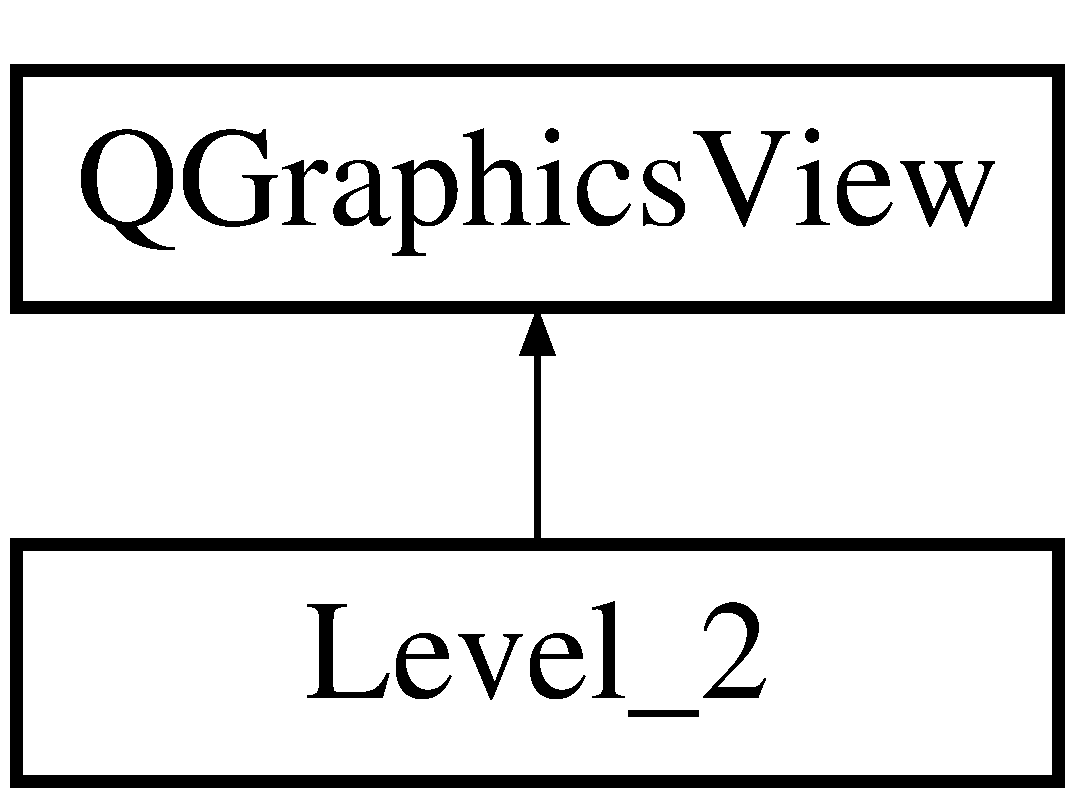
\includegraphics[height=2.000000cm]{class_level__2}
\end{center}
\end{figure}
\subsection*{Public Slots}
\begin{DoxyCompactItemize}
\item 
void \hyperlink{class_level__2_aecda66f24b228432774b66622e357b79}{update} ()
\begin{DoxyCompactList}\small\item\em \hyperlink{class_level__2_aecda66f24b228432774b66622e357b79}{Level\+\_\+2\+::update} update function for moveable objects like our ball -\/ sets the graphics of the ball to the position of the box2D body. \end{DoxyCompactList}\item 
void \hyperlink{class_level__2_af352796cec648d1624950c4d808fe70a}{start\+Level} ()
\begin{DoxyCompactList}\small\item\em \hyperlink{class_level__2_af352796cec648d1624950c4d808fe70a}{Level\+\_\+2\+::start\+Level} Set the flag of the Q\+Graphics\+Item, after start was clicked. draw the graphics if the body was moved before start was clicked. \end{DoxyCompactList}\item 
void \hyperlink{class_level__2_a56bca78ab9033cc0b9b59956f6437c01}{pause\+Level} ()
\begin{DoxyCompactList}\small\item\em \hyperlink{class_level__2_a56bca78ab9033cc0b9b59956f6437c01}{Level\+\_\+2\+::pause\+Level} pauses game when button pause is clicked. \end{DoxyCompactList}\item 
void \hyperlink{class_level__2_a85cd30430d11639814073448ff5f7324}{resume\+Level} ()
\begin{DoxyCompactList}\small\item\em \hyperlink{class_level__2_a85cd30430d11639814073448ff5f7324}{Level\+\_\+2\+::resume\+Level} resumes game when button resume is clicked. \end{DoxyCompactList}\item 
void \hyperlink{class_level__2_afa0a501ea656c0bf83f4bdf9604681cf}{add\+Rectangle} ()
\begin{DoxyCompactList}\small\item\em \hyperlink{class_level__2_afa0a501ea656c0bf83f4bdf9604681cf}{Level\+\_\+2\+::add\+Rectangle} Create new rectangle and count the rectangle items. limited to number. \end{DoxyCompactList}\item 
void \hyperlink{class_level__2_a9b615ad4bcbc5aefaede84a0b5c1a9ff}{add\+Circle} ()
\begin{DoxyCompactList}\small\item\em \hyperlink{class_level__2_a9b615ad4bcbc5aefaede84a0b5c1a9ff}{Level\+\_\+2\+::add\+Circle} Create new \hyperlink{class_circle}{Circle} and count the circle items. Limited to number. \end{DoxyCompactList}\item 
void \hyperlink{class_level__2_abfc4e2bc8eace6aa74d00f61b15b2f52}{add\+Triangle} ()
\begin{DoxyCompactList}\small\item\em \hyperlink{class_level__2_abfc4e2bc8eace6aa74d00f61b15b2f52}{Level\+\_\+2\+::add\+Triangle} Create new \hyperlink{class_triangle}{Triangle} and count the triangle items. Limited to number. \end{DoxyCompactList}\item 
void \hyperlink{class_level__2_a698527f9393e2564eaf01144bfa71503}{reset} ()
\begin{DoxyCompactList}\small\item\em \hyperlink{class_level__2_a698527f9393e2564eaf01144bfa71503}{Level\+\_\+2\+::reset} Clear scene and load Level again. \end{DoxyCompactList}\item 
void \hyperlink{class_level__2_a9a92532482579a062583248529369cfa}{close\+Level} ()
\begin{DoxyCompactList}\small\item\em \hyperlink{class_level__2_a9a92532482579a062583248529369cfa}{Level\+\_\+2\+::close\+Level} if Q\+Graphics\+View is closed emit Signal. \end{DoxyCompactList}\item 
void \hyperlink{class_level__2_a3164141a1c668eef4c9288761de4ae45}{rotate\+Left} ()
\begin{DoxyCompactList}\small\item\em \hyperlink{class_level__2_a3164141a1c668eef4c9288761de4ae45}{Level\+\_\+2\+::rotate\+Left} possibility to rotate objects to the left. \end{DoxyCompactList}\item 
void \hyperlink{class_level__2_a67eacf68f6bbb66220b9ab8760ed90e1}{rotate\+Right} ()
\begin{DoxyCompactList}\small\item\em \hyperlink{class_level__2_a67eacf68f6bbb66220b9ab8760ed90e1}{Level\+\_\+2\+::rotate\+Right} possibility to rotate right. \end{DoxyCompactList}\item 
void \hyperlink{class_level__2_a1803f60231c74fd237d37212a97e7eb6}{get\+Time} ()
\begin{DoxyCompactList}\small\item\em \hyperlink{class_level__2_a1803f60231c74fd237d37212a97e7eb6}{Level\+\_\+2\+::get\+Time} Stop time and convert it to ms. \end{DoxyCompactList}\item 
void \hyperlink{class_level__2_a11fcf461308346ff34e2f6bac7f58476}{highscore\+Counter} ()
\begin{DoxyCompactList}\small\item\em \hyperlink{class_level__2_a11fcf461308346ff34e2f6bac7f58476}{Level\+\_\+2\+::highscore\+Counter} Calculate the highscore. \end{DoxyCompactList}\end{DoxyCompactItemize}
\subsection*{Signals}
\begin{DoxyCompactItemize}
\item 
void \hyperlink{class_level__2_a29c182a385cb5c4036e41ff17a129e56}{levelcompleted} ()
\end{DoxyCompactItemize}
\subsection*{Public Member Functions}
\begin{DoxyCompactItemize}
\item 
\hyperlink{class_level__2_ad9e1165b1cf042f4d2c7337d25fc65e9}{Level\+\_\+2} ()
\begin{DoxyCompactList}\small\item\em \hyperlink{class_level__2_ad9e1165b1cf042f4d2c7337d25fc65e9}{Level\+\_\+2\+::\+Level\+\_\+2} Initialize Level1 -\/ Screen/\+Scene Setup... \end{DoxyCompactList}\end{DoxyCompactItemize}
\subsection*{Public Attributes}
\begin{DoxyCompactItemize}
\item 
std\+::vector$<$ \hyperlink{class_block}{Block} $\ast$ $>$ \hyperlink{class_level__2_aaba33e2422ee9c077787c13912ddf05f}{vectb}
\item 
std\+::vector$<$ \hyperlink{class_triangle}{Triangle} $\ast$ $>$ \hyperlink{class_level__2_ad1367daaa96a8c50955eb735a3606dde}{vectt}
\end{DoxyCompactItemize}


\subsection{Constructor \& Destructor Documentation}
\index{Level\+\_\+2@{Level\+\_\+2}!Level\+\_\+2@{Level\+\_\+2}}
\index{Level\+\_\+2@{Level\+\_\+2}!Level\+\_\+2@{Level\+\_\+2}}
\subsubsection[{\texorpdfstring{Level\+\_\+2()}{Level_2()}}]{\setlength{\rightskip}{0pt plus 5cm}Level\+\_\+2\+::\+Level\+\_\+2 (
\begin{DoxyParamCaption}
{}
\end{DoxyParamCaption}
)}\hypertarget{class_level__2_ad9e1165b1cf042f4d2c7337d25fc65e9}{}\label{class_level__2_ad9e1165b1cf042f4d2c7337d25fc65e9}


\hyperlink{class_level__2_ad9e1165b1cf042f4d2c7337d25fc65e9}{Level\+\_\+2\+::\+Level\+\_\+2} Initialize Level1 -\/ Screen/\+Scene Setup... 

Set Application-\/\+Name 

\subsection{Member Function Documentation}
\index{Level\+\_\+2@{Level\+\_\+2}!add\+Circle@{add\+Circle}}
\index{add\+Circle@{add\+Circle}!Level\+\_\+2@{Level\+\_\+2}}
\subsubsection[{\texorpdfstring{add\+Circle}{addCircle}}]{\setlength{\rightskip}{0pt plus 5cm}void Level\+\_\+2\+::add\+Circle (
\begin{DoxyParamCaption}
{}
\end{DoxyParamCaption}
)\hspace{0.3cm}{\ttfamily [slot]}}\hypertarget{class_level__2_a9b615ad4bcbc5aefaede84a0b5c1a9ff}{}\label{class_level__2_a9b615ad4bcbc5aefaede84a0b5c1a9ff}


\hyperlink{class_level__2_a9b615ad4bcbc5aefaede84a0b5c1a9ff}{Level\+\_\+2\+::add\+Circle} Create new \hyperlink{class_circle}{Circle} and count the circle items. Limited to number. 

\index{Level\+\_\+2@{Level\+\_\+2}!add\+Rectangle@{add\+Rectangle}}
\index{add\+Rectangle@{add\+Rectangle}!Level\+\_\+2@{Level\+\_\+2}}
\subsubsection[{\texorpdfstring{add\+Rectangle}{addRectangle}}]{\setlength{\rightskip}{0pt plus 5cm}void Level\+\_\+2\+::add\+Rectangle (
\begin{DoxyParamCaption}
{}
\end{DoxyParamCaption}
)\hspace{0.3cm}{\ttfamily [slot]}}\hypertarget{class_level__2_afa0a501ea656c0bf83f4bdf9604681cf}{}\label{class_level__2_afa0a501ea656c0bf83f4bdf9604681cf}


\hyperlink{class_level__2_afa0a501ea656c0bf83f4bdf9604681cf}{Level\+\_\+2\+::add\+Rectangle} Create new rectangle and count the rectangle items. limited to number. 

\index{Level\+\_\+2@{Level\+\_\+2}!add\+Triangle@{add\+Triangle}}
\index{add\+Triangle@{add\+Triangle}!Level\+\_\+2@{Level\+\_\+2}}
\subsubsection[{\texorpdfstring{add\+Triangle}{addTriangle}}]{\setlength{\rightskip}{0pt plus 5cm}void Level\+\_\+2\+::add\+Triangle (
\begin{DoxyParamCaption}
{}
\end{DoxyParamCaption}
)\hspace{0.3cm}{\ttfamily [slot]}}\hypertarget{class_level__2_abfc4e2bc8eace6aa74d00f61b15b2f52}{}\label{class_level__2_abfc4e2bc8eace6aa74d00f61b15b2f52}


\hyperlink{class_level__2_abfc4e2bc8eace6aa74d00f61b15b2f52}{Level\+\_\+2\+::add\+Triangle} Create new \hyperlink{class_triangle}{Triangle} and count the triangle items. Limited to number. 

\index{Level\+\_\+2@{Level\+\_\+2}!close\+Level@{close\+Level}}
\index{close\+Level@{close\+Level}!Level\+\_\+2@{Level\+\_\+2}}
\subsubsection[{\texorpdfstring{close\+Level}{closeLevel}}]{\setlength{\rightskip}{0pt plus 5cm}void Level\+\_\+2\+::close\+Level (
\begin{DoxyParamCaption}
{}
\end{DoxyParamCaption}
)\hspace{0.3cm}{\ttfamily [slot]}}\hypertarget{class_level__2_a9a92532482579a062583248529369cfa}{}\label{class_level__2_a9a92532482579a062583248529369cfa}


\hyperlink{class_level__2_a9a92532482579a062583248529369cfa}{Level\+\_\+2\+::close\+Level} if Q\+Graphics\+View is closed emit Signal. 

\index{Level\+\_\+2@{Level\+\_\+2}!get\+Time@{get\+Time}}
\index{get\+Time@{get\+Time}!Level\+\_\+2@{Level\+\_\+2}}
\subsubsection[{\texorpdfstring{get\+Time}{getTime}}]{\setlength{\rightskip}{0pt plus 5cm}void Level\+\_\+2\+::get\+Time (
\begin{DoxyParamCaption}
{}
\end{DoxyParamCaption}
)\hspace{0.3cm}{\ttfamily [slot]}}\hypertarget{class_level__2_a1803f60231c74fd237d37212a97e7eb6}{}\label{class_level__2_a1803f60231c74fd237d37212a97e7eb6}


\hyperlink{class_level__2_a1803f60231c74fd237d37212a97e7eb6}{Level\+\_\+2\+::get\+Time} Stop time and convert it to ms. 

\index{Level\+\_\+2@{Level\+\_\+2}!highscore\+Counter@{highscore\+Counter}}
\index{highscore\+Counter@{highscore\+Counter}!Level\+\_\+2@{Level\+\_\+2}}
\subsubsection[{\texorpdfstring{highscore\+Counter}{highscoreCounter}}]{\setlength{\rightskip}{0pt plus 5cm}void Level\+\_\+2\+::highscore\+Counter (
\begin{DoxyParamCaption}
{}
\end{DoxyParamCaption}
)\hspace{0.3cm}{\ttfamily [slot]}}\hypertarget{class_level__2_a11fcf461308346ff34e2f6bac7f58476}{}\label{class_level__2_a11fcf461308346ff34e2f6bac7f58476}


\hyperlink{class_level__2_a11fcf461308346ff34e2f6bac7f58476}{Level\+\_\+2\+::highscore\+Counter} Calculate the highscore. 

\index{Level\+\_\+2@{Level\+\_\+2}!levelcompleted@{levelcompleted}}
\index{levelcompleted@{levelcompleted}!Level\+\_\+2@{Level\+\_\+2}}
\subsubsection[{\texorpdfstring{levelcompleted}{levelcompleted}}]{\setlength{\rightskip}{0pt plus 5cm}void Level\+\_\+2\+::levelcompleted (
\begin{DoxyParamCaption}
{}
\end{DoxyParamCaption}
)\hspace{0.3cm}{\ttfamily [signal]}}\hypertarget{class_level__2_a29c182a385cb5c4036e41ff17a129e56}{}\label{class_level__2_a29c182a385cb5c4036e41ff17a129e56}
\index{Level\+\_\+2@{Level\+\_\+2}!pause\+Level@{pause\+Level}}
\index{pause\+Level@{pause\+Level}!Level\+\_\+2@{Level\+\_\+2}}
\subsubsection[{\texorpdfstring{pause\+Level}{pauseLevel}}]{\setlength{\rightskip}{0pt plus 5cm}void Level\+\_\+2\+::pause\+Level (
\begin{DoxyParamCaption}
{}
\end{DoxyParamCaption}
)\hspace{0.3cm}{\ttfamily [slot]}}\hypertarget{class_level__2_a56bca78ab9033cc0b9b59956f6437c01}{}\label{class_level__2_a56bca78ab9033cc0b9b59956f6437c01}


\hyperlink{class_level__2_a56bca78ab9033cc0b9b59956f6437c01}{Level\+\_\+2\+::pause\+Level} pauses game when button pause is clicked. 

\index{Level\+\_\+2@{Level\+\_\+2}!reset@{reset}}
\index{reset@{reset}!Level\+\_\+2@{Level\+\_\+2}}
\subsubsection[{\texorpdfstring{reset}{reset}}]{\setlength{\rightskip}{0pt plus 5cm}void Level\+\_\+2\+::reset (
\begin{DoxyParamCaption}
{}
\end{DoxyParamCaption}
)\hspace{0.3cm}{\ttfamily [slot]}}\hypertarget{class_level__2_a698527f9393e2564eaf01144bfa71503}{}\label{class_level__2_a698527f9393e2564eaf01144bfa71503}


\hyperlink{class_level__2_a698527f9393e2564eaf01144bfa71503}{Level\+\_\+2\+::reset} Clear scene and load Level again. 

\index{Level\+\_\+2@{Level\+\_\+2}!resume\+Level@{resume\+Level}}
\index{resume\+Level@{resume\+Level}!Level\+\_\+2@{Level\+\_\+2}}
\subsubsection[{\texorpdfstring{resume\+Level}{resumeLevel}}]{\setlength{\rightskip}{0pt plus 5cm}void Level\+\_\+2\+::resume\+Level (
\begin{DoxyParamCaption}
{}
\end{DoxyParamCaption}
)\hspace{0.3cm}{\ttfamily [slot]}}\hypertarget{class_level__2_a85cd30430d11639814073448ff5f7324}{}\label{class_level__2_a85cd30430d11639814073448ff5f7324}


\hyperlink{class_level__2_a85cd30430d11639814073448ff5f7324}{Level\+\_\+2\+::resume\+Level} resumes game when button resume is clicked. 

\index{Level\+\_\+2@{Level\+\_\+2}!rotate\+Left@{rotate\+Left}}
\index{rotate\+Left@{rotate\+Left}!Level\+\_\+2@{Level\+\_\+2}}
\subsubsection[{\texorpdfstring{rotate\+Left}{rotateLeft}}]{\setlength{\rightskip}{0pt plus 5cm}void Level\+\_\+2\+::rotate\+Left (
\begin{DoxyParamCaption}
{}
\end{DoxyParamCaption}
)\hspace{0.3cm}{\ttfamily [slot]}}\hypertarget{class_level__2_a3164141a1c668eef4c9288761de4ae45}{}\label{class_level__2_a3164141a1c668eef4c9288761de4ae45}


\hyperlink{class_level__2_a3164141a1c668eef4c9288761de4ae45}{Level\+\_\+2\+::rotate\+Left} possibility to rotate objects to the left. 

\index{Level\+\_\+2@{Level\+\_\+2}!rotate\+Right@{rotate\+Right}}
\index{rotate\+Right@{rotate\+Right}!Level\+\_\+2@{Level\+\_\+2}}
\subsubsection[{\texorpdfstring{rotate\+Right}{rotateRight}}]{\setlength{\rightskip}{0pt plus 5cm}void Level\+\_\+2\+::rotate\+Right (
\begin{DoxyParamCaption}
{}
\end{DoxyParamCaption}
)\hspace{0.3cm}{\ttfamily [slot]}}\hypertarget{class_level__2_a67eacf68f6bbb66220b9ab8760ed90e1}{}\label{class_level__2_a67eacf68f6bbb66220b9ab8760ed90e1}


\hyperlink{class_level__2_a67eacf68f6bbb66220b9ab8760ed90e1}{Level\+\_\+2\+::rotate\+Right} possibility to rotate right. 

\index{Level\+\_\+2@{Level\+\_\+2}!start\+Level@{start\+Level}}
\index{start\+Level@{start\+Level}!Level\+\_\+2@{Level\+\_\+2}}
\subsubsection[{\texorpdfstring{start\+Level}{startLevel}}]{\setlength{\rightskip}{0pt plus 5cm}void Level\+\_\+2\+::start\+Level (
\begin{DoxyParamCaption}
{}
\end{DoxyParamCaption}
)\hspace{0.3cm}{\ttfamily [slot]}}\hypertarget{class_level__2_af352796cec648d1624950c4d808fe70a}{}\label{class_level__2_af352796cec648d1624950c4d808fe70a}


\hyperlink{class_level__2_af352796cec648d1624950c4d808fe70a}{Level\+\_\+2\+::start\+Level} Set the flag of the Q\+Graphics\+Item, after start was clicked. draw the graphics if the body was moved before start was clicked. 

\index{Level\+\_\+2@{Level\+\_\+2}!update@{update}}
\index{update@{update}!Level\+\_\+2@{Level\+\_\+2}}
\subsubsection[{\texorpdfstring{update}{update}}]{\setlength{\rightskip}{0pt plus 5cm}void Level\+\_\+2\+::update (
\begin{DoxyParamCaption}
{}
\end{DoxyParamCaption}
)\hspace{0.3cm}{\ttfamily [slot]}}\hypertarget{class_level__2_aecda66f24b228432774b66622e357b79}{}\label{class_level__2_aecda66f24b228432774b66622e357b79}


\hyperlink{class_level__2_aecda66f24b228432774b66622e357b79}{Level\+\_\+2\+::update} update function for moveable objects like our ball -\/ sets the graphics of the ball to the position of the box2D body. 



\subsection{Member Data Documentation}
\index{Level\+\_\+2@{Level\+\_\+2}!vectb@{vectb}}
\index{vectb@{vectb}!Level\+\_\+2@{Level\+\_\+2}}
\subsubsection[{\texorpdfstring{vectb}{vectb}}]{\setlength{\rightskip}{0pt plus 5cm}std\+::vector$<${\bf Block}$\ast$$>$ Level\+\_\+2\+::vectb}\hypertarget{class_level__2_aaba33e2422ee9c077787c13912ddf05f}{}\label{class_level__2_aaba33e2422ee9c077787c13912ddf05f}
\index{Level\+\_\+2@{Level\+\_\+2}!vectt@{vectt}}
\index{vectt@{vectt}!Level\+\_\+2@{Level\+\_\+2}}
\subsubsection[{\texorpdfstring{vectt}{vectt}}]{\setlength{\rightskip}{0pt plus 5cm}std\+::vector$<${\bf Triangle}$\ast$$>$ Level\+\_\+2\+::vectt}\hypertarget{class_level__2_ad1367daaa96a8c50955eb735a3606dde}{}\label{class_level__2_ad1367daaa96a8c50955eb735a3606dde}


The documentation for this class was generated from the following files\+:\begin{DoxyCompactItemize}
\item 
Game/\hyperlink{level__2_8h}{level\+\_\+2.\+h}\item 
Game/\hyperlink{level__2_8cpp}{level\+\_\+2.\+cpp}\end{DoxyCompactItemize}

\hypertarget{class_level__3}{}\section{Level\+\_\+3 Class Reference}
\label{class_level__3}\index{Level\+\_\+3@{Level\+\_\+3}}


{\ttfamily \#include $<$level\+\_\+3.\+h$>$}

Inheritance diagram for Level\+\_\+3\+:\begin{figure}[H]
\begin{center}
\leavevmode
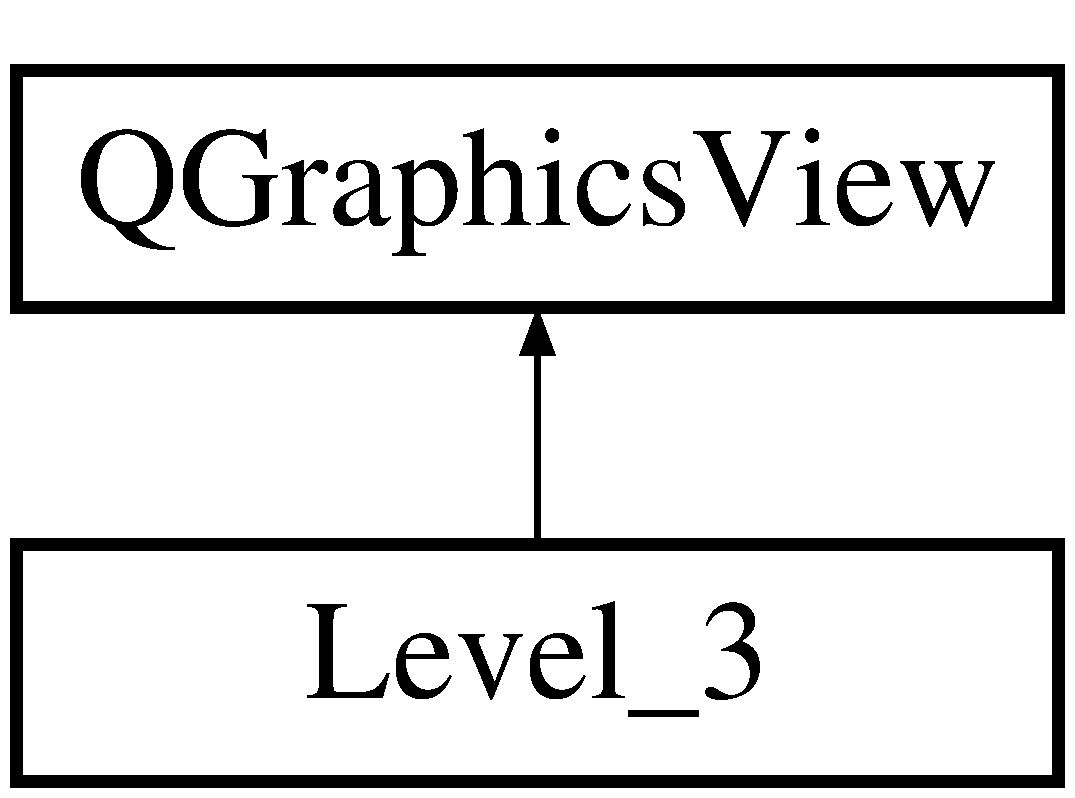
\includegraphics[height=2.000000cm]{class_level__3}
\end{center}
\end{figure}
\subsection*{Public Slots}
\begin{DoxyCompactItemize}
\item 
void \hyperlink{class_level__3_ade0e1a21028d3e2b131e746be449c104}{update} ()
\begin{DoxyCompactList}\small\item\em \hyperlink{class_level__3_ade0e1a21028d3e2b131e746be449c104}{Level\+\_\+3\+::update} update function for moveable objects like our ball -\/ sets the graphics of the ball to the position of the box2D body. \end{DoxyCompactList}\item 
void \hyperlink{class_level__3_a568dd8e058966a0bd0a0244ef39113df}{start\+Level} ()
\begin{DoxyCompactList}\small\item\em \hyperlink{class_level__3_a568dd8e058966a0bd0a0244ef39113df}{Level\+\_\+3\+::start\+Level} Set the flag of the Q\+Graphics\+Item, after start was clicked. draw the graphics if the body was moved before start was clicked. \end{DoxyCompactList}\item 
void \hyperlink{class_level__3_ac728b5d2a33a179ddfc4c61246d8ef52}{pause\+Level} ()
\begin{DoxyCompactList}\small\item\em \hyperlink{class_level__3_ac728b5d2a33a179ddfc4c61246d8ef52}{Level\+\_\+3\+::pause\+Level} pauses game when button pause is clicked. \end{DoxyCompactList}\item 
void \hyperlink{class_level__3_a7e63baefd91e5be5309500299060788a}{resume\+Level} ()
\begin{DoxyCompactList}\small\item\em \hyperlink{class_level__3_a7e63baefd91e5be5309500299060788a}{Level\+\_\+3\+::resume\+Level} resumes game when button resume is clicked. \end{DoxyCompactList}\item 
void \hyperlink{class_level__3_a98abb4e9bc67098461cfa4b43928c430}{add\+Rectangle} ()
\begin{DoxyCompactList}\small\item\em \hyperlink{class_level__3_a98abb4e9bc67098461cfa4b43928c430}{Level\+\_\+3\+::add\+Rectangle} Create new rectangle and count the rectangle items. limited to number. \end{DoxyCompactList}\item 
void \hyperlink{class_level__3_a98d333c23eaa04449be0325fac0ce5c5}{add\+Circle} ()
\begin{DoxyCompactList}\small\item\em \hyperlink{class_level__3_a98d333c23eaa04449be0325fac0ce5c5}{Level\+\_\+3\+::add\+Circle} Create new \hyperlink{class_circle}{Circle} and count the circle items. Limited to number. \end{DoxyCompactList}\item 
void \hyperlink{class_level__3_ad64679db61e97bde32906ed4e510e8da}{add\+Triangle} ()
\begin{DoxyCompactList}\small\item\em \hyperlink{class_level__3_ad64679db61e97bde32906ed4e510e8da}{Level\+\_\+3\+::add\+Triangle} Create new \hyperlink{class_triangle}{Triangle} and count the triangle items. Limited to number. \end{DoxyCompactList}\item 
void \hyperlink{class_level__3_af2a31fd327d12dd2f8fa866ecdf6a921}{reset} ()
\begin{DoxyCompactList}\small\item\em \hyperlink{class_level__3_af2a31fd327d12dd2f8fa866ecdf6a921}{Level\+\_\+3\+::reset} Clear scene and load Level again. \end{DoxyCompactList}\item 
void \hyperlink{class_level__3_a0a558cf0328b8f34e6937c8f36e63741}{close\+Level} ()
\begin{DoxyCompactList}\small\item\em \hyperlink{class_level__3_a0a558cf0328b8f34e6937c8f36e63741}{Level\+\_\+3\+::close\+Level} if Q\+Graphics\+View is closed emit Signal. \end{DoxyCompactList}\item 
void \hyperlink{class_level__3_a0887d7c8cf7f71dddae0ee8be21ee669}{rotate\+Left} ()
\begin{DoxyCompactList}\small\item\em \hyperlink{class_level__3_a0887d7c8cf7f71dddae0ee8be21ee669}{Level\+\_\+3\+::rotate\+Left} possibility to rotate objects to the left. \end{DoxyCompactList}\item 
void \hyperlink{class_level__3_a8caf89fa6bbdefd52a091688b5a4e752}{rotate\+Right} ()
\begin{DoxyCompactList}\small\item\em \hyperlink{class_level__3_a8caf89fa6bbdefd52a091688b5a4e752}{Level\+\_\+3\+::rotate\+Right} possibility to rotate right. \end{DoxyCompactList}\item 
void \hyperlink{class_level__3_aa1d44955dd59963e69e219799250d88f}{get\+Time} ()
\begin{DoxyCompactList}\small\item\em \hyperlink{class_level__3_aa1d44955dd59963e69e219799250d88f}{Level\+\_\+3\+::get\+Time} Stop time and convert it to ms. \end{DoxyCompactList}\item 
void \hyperlink{class_level__3_aa4fdb9a87496d123fb3b7714af46671d}{highscore\+Counter} ()
\begin{DoxyCompactList}\small\item\em \hyperlink{class_level__3_aa4fdb9a87496d123fb3b7714af46671d}{Level\+\_\+3\+::highscore\+Counter} Calculate the highscore. \end{DoxyCompactList}\end{DoxyCompactItemize}
\subsection*{Signals}
\begin{DoxyCompactItemize}
\item 
void \hyperlink{class_level__3_afddb9bbefea55ef7f824f2a7d7d29f6e}{levelcompleted} ()
\end{DoxyCompactItemize}
\subsection*{Public Member Functions}
\begin{DoxyCompactItemize}
\item 
\hyperlink{class_level__3_a79305de54e6426adf09b4cfb6d272845}{Level\+\_\+3} ()
\begin{DoxyCompactList}\small\item\em \hyperlink{class_level__3_a79305de54e6426adf09b4cfb6d272845}{Level\+\_\+3\+::\+Level\+\_\+3} Initialize Level1 -\/ Screen/\+Scene Setup... \end{DoxyCompactList}\end{DoxyCompactItemize}


\subsection{Constructor \& Destructor Documentation}
\index{Level\+\_\+3@{Level\+\_\+3}!Level\+\_\+3@{Level\+\_\+3}}
\index{Level\+\_\+3@{Level\+\_\+3}!Level\+\_\+3@{Level\+\_\+3}}
\subsubsection[{\texorpdfstring{Level\+\_\+3()}{Level_3()}}]{\setlength{\rightskip}{0pt plus 5cm}Level\+\_\+3\+::\+Level\+\_\+3 (
\begin{DoxyParamCaption}
{}
\end{DoxyParamCaption}
)}\hypertarget{class_level__3_a79305de54e6426adf09b4cfb6d272845}{}\label{class_level__3_a79305de54e6426adf09b4cfb6d272845}


\hyperlink{class_level__3_a79305de54e6426adf09b4cfb6d272845}{Level\+\_\+3\+::\+Level\+\_\+3} Initialize Level1 -\/ Screen/\+Scene Setup... 

Set Application-\/\+Name 

\subsection{Member Function Documentation}
\index{Level\+\_\+3@{Level\+\_\+3}!add\+Circle@{add\+Circle}}
\index{add\+Circle@{add\+Circle}!Level\+\_\+3@{Level\+\_\+3}}
\subsubsection[{\texorpdfstring{add\+Circle}{addCircle}}]{\setlength{\rightskip}{0pt plus 5cm}void Level\+\_\+3\+::add\+Circle (
\begin{DoxyParamCaption}
{}
\end{DoxyParamCaption}
)\hspace{0.3cm}{\ttfamily [slot]}}\hypertarget{class_level__3_a98d333c23eaa04449be0325fac0ce5c5}{}\label{class_level__3_a98d333c23eaa04449be0325fac0ce5c5}


\hyperlink{class_level__3_a98d333c23eaa04449be0325fac0ce5c5}{Level\+\_\+3\+::add\+Circle} Create new \hyperlink{class_circle}{Circle} and count the circle items. Limited to number. 

\index{Level\+\_\+3@{Level\+\_\+3}!add\+Rectangle@{add\+Rectangle}}
\index{add\+Rectangle@{add\+Rectangle}!Level\+\_\+3@{Level\+\_\+3}}
\subsubsection[{\texorpdfstring{add\+Rectangle}{addRectangle}}]{\setlength{\rightskip}{0pt plus 5cm}void Level\+\_\+3\+::add\+Rectangle (
\begin{DoxyParamCaption}
{}
\end{DoxyParamCaption}
)\hspace{0.3cm}{\ttfamily [slot]}}\hypertarget{class_level__3_a98abb4e9bc67098461cfa4b43928c430}{}\label{class_level__3_a98abb4e9bc67098461cfa4b43928c430}


\hyperlink{class_level__3_a98abb4e9bc67098461cfa4b43928c430}{Level\+\_\+3\+::add\+Rectangle} Create new rectangle and count the rectangle items. limited to number. 

\index{Level\+\_\+3@{Level\+\_\+3}!add\+Triangle@{add\+Triangle}}
\index{add\+Triangle@{add\+Triangle}!Level\+\_\+3@{Level\+\_\+3}}
\subsubsection[{\texorpdfstring{add\+Triangle}{addTriangle}}]{\setlength{\rightskip}{0pt plus 5cm}void Level\+\_\+3\+::add\+Triangle (
\begin{DoxyParamCaption}
{}
\end{DoxyParamCaption}
)\hspace{0.3cm}{\ttfamily [slot]}}\hypertarget{class_level__3_ad64679db61e97bde32906ed4e510e8da}{}\label{class_level__3_ad64679db61e97bde32906ed4e510e8da}


\hyperlink{class_level__3_ad64679db61e97bde32906ed4e510e8da}{Level\+\_\+3\+::add\+Triangle} Create new \hyperlink{class_triangle}{Triangle} and count the triangle items. Limited to number. 

\index{Level\+\_\+3@{Level\+\_\+3}!close\+Level@{close\+Level}}
\index{close\+Level@{close\+Level}!Level\+\_\+3@{Level\+\_\+3}}
\subsubsection[{\texorpdfstring{close\+Level}{closeLevel}}]{\setlength{\rightskip}{0pt plus 5cm}void Level\+\_\+3\+::close\+Level (
\begin{DoxyParamCaption}
{}
\end{DoxyParamCaption}
)\hspace{0.3cm}{\ttfamily [slot]}}\hypertarget{class_level__3_a0a558cf0328b8f34e6937c8f36e63741}{}\label{class_level__3_a0a558cf0328b8f34e6937c8f36e63741}


\hyperlink{class_level__3_a0a558cf0328b8f34e6937c8f36e63741}{Level\+\_\+3\+::close\+Level} if Q\+Graphics\+View is closed emit Signal. 

\index{Level\+\_\+3@{Level\+\_\+3}!get\+Time@{get\+Time}}
\index{get\+Time@{get\+Time}!Level\+\_\+3@{Level\+\_\+3}}
\subsubsection[{\texorpdfstring{get\+Time}{getTime}}]{\setlength{\rightskip}{0pt plus 5cm}void Level\+\_\+3\+::get\+Time (
\begin{DoxyParamCaption}
{}
\end{DoxyParamCaption}
)\hspace{0.3cm}{\ttfamily [slot]}}\hypertarget{class_level__3_aa1d44955dd59963e69e219799250d88f}{}\label{class_level__3_aa1d44955dd59963e69e219799250d88f}


\hyperlink{class_level__3_aa1d44955dd59963e69e219799250d88f}{Level\+\_\+3\+::get\+Time} Stop time and convert it to ms. 

\index{Level\+\_\+3@{Level\+\_\+3}!highscore\+Counter@{highscore\+Counter}}
\index{highscore\+Counter@{highscore\+Counter}!Level\+\_\+3@{Level\+\_\+3}}
\subsubsection[{\texorpdfstring{highscore\+Counter}{highscoreCounter}}]{\setlength{\rightskip}{0pt plus 5cm}void Level\+\_\+3\+::highscore\+Counter (
\begin{DoxyParamCaption}
{}
\end{DoxyParamCaption}
)\hspace{0.3cm}{\ttfamily [slot]}}\hypertarget{class_level__3_aa4fdb9a87496d123fb3b7714af46671d}{}\label{class_level__3_aa4fdb9a87496d123fb3b7714af46671d}


\hyperlink{class_level__3_aa4fdb9a87496d123fb3b7714af46671d}{Level\+\_\+3\+::highscore\+Counter} Calculate the highscore. 

\index{Level\+\_\+3@{Level\+\_\+3}!levelcompleted@{levelcompleted}}
\index{levelcompleted@{levelcompleted}!Level\+\_\+3@{Level\+\_\+3}}
\subsubsection[{\texorpdfstring{levelcompleted}{levelcompleted}}]{\setlength{\rightskip}{0pt plus 5cm}void Level\+\_\+3\+::levelcompleted (
\begin{DoxyParamCaption}
{}
\end{DoxyParamCaption}
)\hspace{0.3cm}{\ttfamily [signal]}}\hypertarget{class_level__3_afddb9bbefea55ef7f824f2a7d7d29f6e}{}\label{class_level__3_afddb9bbefea55ef7f824f2a7d7d29f6e}
\index{Level\+\_\+3@{Level\+\_\+3}!pause\+Level@{pause\+Level}}
\index{pause\+Level@{pause\+Level}!Level\+\_\+3@{Level\+\_\+3}}
\subsubsection[{\texorpdfstring{pause\+Level}{pauseLevel}}]{\setlength{\rightskip}{0pt plus 5cm}void Level\+\_\+3\+::pause\+Level (
\begin{DoxyParamCaption}
{}
\end{DoxyParamCaption}
)\hspace{0.3cm}{\ttfamily [slot]}}\hypertarget{class_level__3_ac728b5d2a33a179ddfc4c61246d8ef52}{}\label{class_level__3_ac728b5d2a33a179ddfc4c61246d8ef52}


\hyperlink{class_level__3_ac728b5d2a33a179ddfc4c61246d8ef52}{Level\+\_\+3\+::pause\+Level} pauses game when button pause is clicked. 

\index{Level\+\_\+3@{Level\+\_\+3}!reset@{reset}}
\index{reset@{reset}!Level\+\_\+3@{Level\+\_\+3}}
\subsubsection[{\texorpdfstring{reset}{reset}}]{\setlength{\rightskip}{0pt plus 5cm}void Level\+\_\+3\+::reset (
\begin{DoxyParamCaption}
{}
\end{DoxyParamCaption}
)\hspace{0.3cm}{\ttfamily [slot]}}\hypertarget{class_level__3_af2a31fd327d12dd2f8fa866ecdf6a921}{}\label{class_level__3_af2a31fd327d12dd2f8fa866ecdf6a921}


\hyperlink{class_level__3_af2a31fd327d12dd2f8fa866ecdf6a921}{Level\+\_\+3\+::reset} Clear scene and load Level again. 

\index{Level\+\_\+3@{Level\+\_\+3}!resume\+Level@{resume\+Level}}
\index{resume\+Level@{resume\+Level}!Level\+\_\+3@{Level\+\_\+3}}
\subsubsection[{\texorpdfstring{resume\+Level}{resumeLevel}}]{\setlength{\rightskip}{0pt plus 5cm}void Level\+\_\+3\+::resume\+Level (
\begin{DoxyParamCaption}
{}
\end{DoxyParamCaption}
)\hspace{0.3cm}{\ttfamily [slot]}}\hypertarget{class_level__3_a7e63baefd91e5be5309500299060788a}{}\label{class_level__3_a7e63baefd91e5be5309500299060788a}


\hyperlink{class_level__3_a7e63baefd91e5be5309500299060788a}{Level\+\_\+3\+::resume\+Level} resumes game when button resume is clicked. 

\index{Level\+\_\+3@{Level\+\_\+3}!rotate\+Left@{rotate\+Left}}
\index{rotate\+Left@{rotate\+Left}!Level\+\_\+3@{Level\+\_\+3}}
\subsubsection[{\texorpdfstring{rotate\+Left}{rotateLeft}}]{\setlength{\rightskip}{0pt plus 5cm}void Level\+\_\+3\+::rotate\+Left (
\begin{DoxyParamCaption}
{}
\end{DoxyParamCaption}
)\hspace{0.3cm}{\ttfamily [slot]}}\hypertarget{class_level__3_a0887d7c8cf7f71dddae0ee8be21ee669}{}\label{class_level__3_a0887d7c8cf7f71dddae0ee8be21ee669}


\hyperlink{class_level__3_a0887d7c8cf7f71dddae0ee8be21ee669}{Level\+\_\+3\+::rotate\+Left} possibility to rotate objects to the left. 

\index{Level\+\_\+3@{Level\+\_\+3}!rotate\+Right@{rotate\+Right}}
\index{rotate\+Right@{rotate\+Right}!Level\+\_\+3@{Level\+\_\+3}}
\subsubsection[{\texorpdfstring{rotate\+Right}{rotateRight}}]{\setlength{\rightskip}{0pt plus 5cm}void Level\+\_\+3\+::rotate\+Right (
\begin{DoxyParamCaption}
{}
\end{DoxyParamCaption}
)\hspace{0.3cm}{\ttfamily [slot]}}\hypertarget{class_level__3_a8caf89fa6bbdefd52a091688b5a4e752}{}\label{class_level__3_a8caf89fa6bbdefd52a091688b5a4e752}


\hyperlink{class_level__3_a8caf89fa6bbdefd52a091688b5a4e752}{Level\+\_\+3\+::rotate\+Right} possibility to rotate right. 

\index{Level\+\_\+3@{Level\+\_\+3}!start\+Level@{start\+Level}}
\index{start\+Level@{start\+Level}!Level\+\_\+3@{Level\+\_\+3}}
\subsubsection[{\texorpdfstring{start\+Level}{startLevel}}]{\setlength{\rightskip}{0pt plus 5cm}void Level\+\_\+3\+::start\+Level (
\begin{DoxyParamCaption}
{}
\end{DoxyParamCaption}
)\hspace{0.3cm}{\ttfamily [slot]}}\hypertarget{class_level__3_a568dd8e058966a0bd0a0244ef39113df}{}\label{class_level__3_a568dd8e058966a0bd0a0244ef39113df}


\hyperlink{class_level__3_a568dd8e058966a0bd0a0244ef39113df}{Level\+\_\+3\+::start\+Level} Set the flag of the Q\+Graphics\+Item, after start was clicked. draw the graphics if the body was moved before start was clicked. 

\index{Level\+\_\+3@{Level\+\_\+3}!update@{update}}
\index{update@{update}!Level\+\_\+3@{Level\+\_\+3}}
\subsubsection[{\texorpdfstring{update}{update}}]{\setlength{\rightskip}{0pt plus 5cm}void Level\+\_\+3\+::update (
\begin{DoxyParamCaption}
{}
\end{DoxyParamCaption}
)\hspace{0.3cm}{\ttfamily [slot]}}\hypertarget{class_level__3_ade0e1a21028d3e2b131e746be449c104}{}\label{class_level__3_ade0e1a21028d3e2b131e746be449c104}


\hyperlink{class_level__3_ade0e1a21028d3e2b131e746be449c104}{Level\+\_\+3\+::update} update function for moveable objects like our ball -\/ sets the graphics of the ball to the position of the box2D body. 



The documentation for this class was generated from the following files\+:\begin{DoxyCompactItemize}
\item 
C\+:/\+Users/\+Maximilian/\+Desktop/\+T\+U\+M/6.\+Semester/\+Grundkurs C++/\+Hauptprojekt/gruppe4\+\_\+hauptprojekt/gruppe4\+\_\+hauptprojekt/\+Game/\hyperlink{level__3_8h}{level\+\_\+3.\+h}\item 
C\+:/\+Users/\+Maximilian/\+Desktop/\+T\+U\+M/6.\+Semester/\+Grundkurs C++/\+Hauptprojekt/gruppe4\+\_\+hauptprojekt/gruppe4\+\_\+hauptprojekt/\+Game/\hyperlink{level__3_8cpp}{level\+\_\+3.\+cpp}\end{DoxyCompactItemize}

\hypertarget{class_level__4}{}\section{Level\+\_\+4 Class Reference}
\label{class_level__4}\index{Level\+\_\+4@{Level\+\_\+4}}


{\ttfamily \#include $<$level\+\_\+4.\+h$>$}

Inheritance diagram for Level\+\_\+4\+:\begin{figure}[H]
\begin{center}
\leavevmode
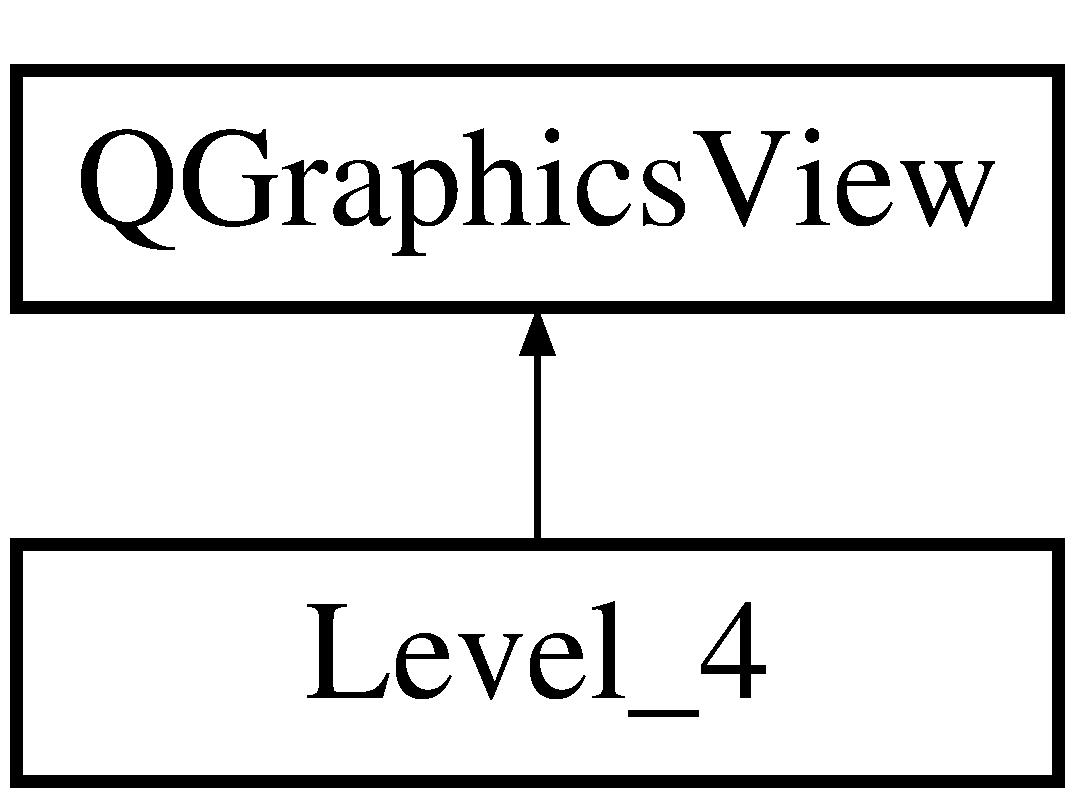
\includegraphics[height=2.000000cm]{class_level__4}
\end{center}
\end{figure}
\subsection*{Public Slots}
\begin{DoxyCompactItemize}
\item 
void \hyperlink{class_level__4_a6feb653af7857552934d71edd3754a49}{update} ()
\begin{DoxyCompactList}\small\item\em \hyperlink{class_level__4_a6feb653af7857552934d71edd3754a49}{Level\+\_\+4\+::update} update function for moveable objects like our ball -\/ sets the graphics of the ball to the position of the box2D body. \end{DoxyCompactList}\item 
void \hyperlink{class_level__4_a1eeca59dfaf2820b1724d0cdbd3e7b81}{start\+Level} ()
\begin{DoxyCompactList}\small\item\em \hyperlink{class_level__4_a1eeca59dfaf2820b1724d0cdbd3e7b81}{Level\+\_\+4\+::start\+Level} Set the flag of the Q\+Graphics\+Item, after start was clicked. draw the graphics if the body was moved before start was clicked. \end{DoxyCompactList}\item 
void \hyperlink{class_level__4_a5d234a430f36904bbe349751bc56b872}{pause\+Level} ()
\begin{DoxyCompactList}\small\item\em \hyperlink{class_level__4_a5d234a430f36904bbe349751bc56b872}{Level\+\_\+4\+::pause\+Level} pauses game when button pause is clicked. \end{DoxyCompactList}\item 
void \hyperlink{class_level__4_aae318a66fee59f389b96fa3d5c6e3d9f}{resume\+Level} ()
\begin{DoxyCompactList}\small\item\em \hyperlink{class_level__4_aae318a66fee59f389b96fa3d5c6e3d9f}{Level\+\_\+4\+::resume\+Level} resumes game when button resume is clicked. \end{DoxyCompactList}\item 
void \hyperlink{class_level__4_a826308245278a309443ce11732632d80}{add\+Rectangle} ()
\begin{DoxyCompactList}\small\item\em \hyperlink{class_level__4_a826308245278a309443ce11732632d80}{Level\+\_\+4\+::add\+Rectangle} Create new rectangle and count the rectangle items. limited to number. \end{DoxyCompactList}\item 
void \hyperlink{class_level__4_a316f33083ed93191bb7160c65e9cb9d6}{add\+Circle} ()
\begin{DoxyCompactList}\small\item\em \hyperlink{class_level__4_a316f33083ed93191bb7160c65e9cb9d6}{Level\+\_\+4\+::add\+Circle} Create new \hyperlink{class_circle}{Circle} and count the circle items. Limited to number. \end{DoxyCompactList}\item 
void \hyperlink{class_level__4_abfc91e29320c89bfa39b9c0547f74ae3}{add\+Triangle} ()
\begin{DoxyCompactList}\small\item\em \hyperlink{class_level__4_abfc91e29320c89bfa39b9c0547f74ae3}{Level\+\_\+4\+::add\+Triangle} Create new \hyperlink{class_triangle}{Triangle} and count the triangle items. Limited to number. \end{DoxyCompactList}\item 
void \hyperlink{class_level__4_ae822c62f61ca12b12ec7246ec5e7f4ad}{reset} ()
\begin{DoxyCompactList}\small\item\em \hyperlink{class_level__4_ae822c62f61ca12b12ec7246ec5e7f4ad}{Level\+\_\+4\+::reset} Clear scene and load Level again. \end{DoxyCompactList}\item 
void \hyperlink{class_level__4_acd9dfb73cd1dcfb72b8dbab35241c654}{close\+Level} ()
\begin{DoxyCompactList}\small\item\em \hyperlink{class_level__4_acd9dfb73cd1dcfb72b8dbab35241c654}{Level\+\_\+4\+::close\+Level} if Q\+Graphics\+View is closed emit Signal. \end{DoxyCompactList}\item 
void \hyperlink{class_level__4_ac7a20e6bb51d1950e64b768bf45582fd}{rotate\+Left} ()
\begin{DoxyCompactList}\small\item\em \hyperlink{class_level__4_ac7a20e6bb51d1950e64b768bf45582fd}{Level\+\_\+4\+::rotate\+Left} possibility to rotate objects to the left. \end{DoxyCompactList}\item 
void \hyperlink{class_level__4_a6751d271128ec2efd3cc17ed76c6f63b}{rotate\+Right} ()
\begin{DoxyCompactList}\small\item\em \hyperlink{class_level__4_a6751d271128ec2efd3cc17ed76c6f63b}{Level\+\_\+4\+::rotate\+Right} possibility to rotate right. \end{DoxyCompactList}\item 
void \hyperlink{class_level__4_a26de79cece6c4608a509536bffdd949b}{get\+Time} ()
\begin{DoxyCompactList}\small\item\em \hyperlink{class_level__4_a26de79cece6c4608a509536bffdd949b}{Level\+\_\+4\+::get\+Time} Stop time and convert it to ms. \end{DoxyCompactList}\item 
void \hyperlink{class_level__4_af2b343d37c3cab79ac019829aec273f5}{highscore\+Counter} ()
\begin{DoxyCompactList}\small\item\em \hyperlink{class_level__4_af2b343d37c3cab79ac019829aec273f5}{Level\+\_\+4\+::highscore\+Counter} Calculate the highscore. \end{DoxyCompactList}\end{DoxyCompactItemize}
\subsection*{Signals}
\begin{DoxyCompactItemize}
\item 
void \hyperlink{class_level__4_a2afa1fbae0eadf9ee46383e85e6bb427}{levelcompleted} ()
\end{DoxyCompactItemize}
\subsection*{Public Member Functions}
\begin{DoxyCompactItemize}
\item 
\hyperlink{class_level__4_a30aa6842c7bac97cace91542d68a9fc5}{Level\+\_\+4} ()
\begin{DoxyCompactList}\small\item\em \hyperlink{class_level__4_a30aa6842c7bac97cace91542d68a9fc5}{Level\+\_\+4\+::\+Level\+\_\+4} Initialize Level1 -\/ Screen/\+Scene Setup... \end{DoxyCompactList}\end{DoxyCompactItemize}
\subsection*{Public Attributes}
\begin{DoxyCompactItemize}
\item 
std\+::vector$<$ \hyperlink{class_block}{Block} $\ast$ $>$ \hyperlink{class_level__4_a7405e54cfaa0373b5114d838f0f39cc7}{vectb}
\item 
std\+::vector$<$ \hyperlink{class_triangle}{Triangle} $\ast$ $>$ \hyperlink{class_level__4_acdd42e79e1b0dbd8bddce42277a20984}{vectt}
\end{DoxyCompactItemize}


\subsection{Constructor \& Destructor Documentation}
\index{Level\+\_\+4@{Level\+\_\+4}!Level\+\_\+4@{Level\+\_\+4}}
\index{Level\+\_\+4@{Level\+\_\+4}!Level\+\_\+4@{Level\+\_\+4}}
\subsubsection[{\texorpdfstring{Level\+\_\+4()}{Level_4()}}]{\setlength{\rightskip}{0pt plus 5cm}Level\+\_\+4\+::\+Level\+\_\+4 (
\begin{DoxyParamCaption}
{}
\end{DoxyParamCaption}
)}\hypertarget{class_level__4_a30aa6842c7bac97cace91542d68a9fc5}{}\label{class_level__4_a30aa6842c7bac97cace91542d68a9fc5}


\hyperlink{class_level__4_a30aa6842c7bac97cace91542d68a9fc5}{Level\+\_\+4\+::\+Level\+\_\+4} Initialize Level1 -\/ Screen/\+Scene Setup... 

Set Application-\/\+Name 

\subsection{Member Function Documentation}
\index{Level\+\_\+4@{Level\+\_\+4}!add\+Circle@{add\+Circle}}
\index{add\+Circle@{add\+Circle}!Level\+\_\+4@{Level\+\_\+4}}
\subsubsection[{\texorpdfstring{add\+Circle}{addCircle}}]{\setlength{\rightskip}{0pt plus 5cm}void Level\+\_\+4\+::add\+Circle (
\begin{DoxyParamCaption}
{}
\end{DoxyParamCaption}
)\hspace{0.3cm}{\ttfamily [slot]}}\hypertarget{class_level__4_a316f33083ed93191bb7160c65e9cb9d6}{}\label{class_level__4_a316f33083ed93191bb7160c65e9cb9d6}


\hyperlink{class_level__4_a316f33083ed93191bb7160c65e9cb9d6}{Level\+\_\+4\+::add\+Circle} Create new \hyperlink{class_circle}{Circle} and count the circle items. Limited to number. 

\index{Level\+\_\+4@{Level\+\_\+4}!add\+Rectangle@{add\+Rectangle}}
\index{add\+Rectangle@{add\+Rectangle}!Level\+\_\+4@{Level\+\_\+4}}
\subsubsection[{\texorpdfstring{add\+Rectangle}{addRectangle}}]{\setlength{\rightskip}{0pt plus 5cm}void Level\+\_\+4\+::add\+Rectangle (
\begin{DoxyParamCaption}
{}
\end{DoxyParamCaption}
)\hspace{0.3cm}{\ttfamily [slot]}}\hypertarget{class_level__4_a826308245278a309443ce11732632d80}{}\label{class_level__4_a826308245278a309443ce11732632d80}


\hyperlink{class_level__4_a826308245278a309443ce11732632d80}{Level\+\_\+4\+::add\+Rectangle} Create new rectangle and count the rectangle items. limited to number. 

\index{Level\+\_\+4@{Level\+\_\+4}!add\+Triangle@{add\+Triangle}}
\index{add\+Triangle@{add\+Triangle}!Level\+\_\+4@{Level\+\_\+4}}
\subsubsection[{\texorpdfstring{add\+Triangle}{addTriangle}}]{\setlength{\rightskip}{0pt plus 5cm}void Level\+\_\+4\+::add\+Triangle (
\begin{DoxyParamCaption}
{}
\end{DoxyParamCaption}
)\hspace{0.3cm}{\ttfamily [slot]}}\hypertarget{class_level__4_abfc91e29320c89bfa39b9c0547f74ae3}{}\label{class_level__4_abfc91e29320c89bfa39b9c0547f74ae3}


\hyperlink{class_level__4_abfc91e29320c89bfa39b9c0547f74ae3}{Level\+\_\+4\+::add\+Triangle} Create new \hyperlink{class_triangle}{Triangle} and count the triangle items. Limited to number. 

\index{Level\+\_\+4@{Level\+\_\+4}!close\+Level@{close\+Level}}
\index{close\+Level@{close\+Level}!Level\+\_\+4@{Level\+\_\+4}}
\subsubsection[{\texorpdfstring{close\+Level}{closeLevel}}]{\setlength{\rightskip}{0pt plus 5cm}void Level\+\_\+4\+::close\+Level (
\begin{DoxyParamCaption}
{}
\end{DoxyParamCaption}
)\hspace{0.3cm}{\ttfamily [slot]}}\hypertarget{class_level__4_acd9dfb73cd1dcfb72b8dbab35241c654}{}\label{class_level__4_acd9dfb73cd1dcfb72b8dbab35241c654}


\hyperlink{class_level__4_acd9dfb73cd1dcfb72b8dbab35241c654}{Level\+\_\+4\+::close\+Level} if Q\+Graphics\+View is closed emit Signal. 

\index{Level\+\_\+4@{Level\+\_\+4}!get\+Time@{get\+Time}}
\index{get\+Time@{get\+Time}!Level\+\_\+4@{Level\+\_\+4}}
\subsubsection[{\texorpdfstring{get\+Time}{getTime}}]{\setlength{\rightskip}{0pt plus 5cm}void Level\+\_\+4\+::get\+Time (
\begin{DoxyParamCaption}
{}
\end{DoxyParamCaption}
)\hspace{0.3cm}{\ttfamily [slot]}}\hypertarget{class_level__4_a26de79cece6c4608a509536bffdd949b}{}\label{class_level__4_a26de79cece6c4608a509536bffdd949b}


\hyperlink{class_level__4_a26de79cece6c4608a509536bffdd949b}{Level\+\_\+4\+::get\+Time} Stop time and convert it to ms. 

\index{Level\+\_\+4@{Level\+\_\+4}!highscore\+Counter@{highscore\+Counter}}
\index{highscore\+Counter@{highscore\+Counter}!Level\+\_\+4@{Level\+\_\+4}}
\subsubsection[{\texorpdfstring{highscore\+Counter}{highscoreCounter}}]{\setlength{\rightskip}{0pt plus 5cm}void Level\+\_\+4\+::highscore\+Counter (
\begin{DoxyParamCaption}
{}
\end{DoxyParamCaption}
)\hspace{0.3cm}{\ttfamily [slot]}}\hypertarget{class_level__4_af2b343d37c3cab79ac019829aec273f5}{}\label{class_level__4_af2b343d37c3cab79ac019829aec273f5}


\hyperlink{class_level__4_af2b343d37c3cab79ac019829aec273f5}{Level\+\_\+4\+::highscore\+Counter} Calculate the highscore. 

\index{Level\+\_\+4@{Level\+\_\+4}!levelcompleted@{levelcompleted}}
\index{levelcompleted@{levelcompleted}!Level\+\_\+4@{Level\+\_\+4}}
\subsubsection[{\texorpdfstring{levelcompleted}{levelcompleted}}]{\setlength{\rightskip}{0pt plus 5cm}void Level\+\_\+4\+::levelcompleted (
\begin{DoxyParamCaption}
{}
\end{DoxyParamCaption}
)\hspace{0.3cm}{\ttfamily [signal]}}\hypertarget{class_level__4_a2afa1fbae0eadf9ee46383e85e6bb427}{}\label{class_level__4_a2afa1fbae0eadf9ee46383e85e6bb427}
\index{Level\+\_\+4@{Level\+\_\+4}!pause\+Level@{pause\+Level}}
\index{pause\+Level@{pause\+Level}!Level\+\_\+4@{Level\+\_\+4}}
\subsubsection[{\texorpdfstring{pause\+Level}{pauseLevel}}]{\setlength{\rightskip}{0pt plus 5cm}void Level\+\_\+4\+::pause\+Level (
\begin{DoxyParamCaption}
{}
\end{DoxyParamCaption}
)\hspace{0.3cm}{\ttfamily [slot]}}\hypertarget{class_level__4_a5d234a430f36904bbe349751bc56b872}{}\label{class_level__4_a5d234a430f36904bbe349751bc56b872}


\hyperlink{class_level__4_a5d234a430f36904bbe349751bc56b872}{Level\+\_\+4\+::pause\+Level} pauses game when button pause is clicked. 

\index{Level\+\_\+4@{Level\+\_\+4}!reset@{reset}}
\index{reset@{reset}!Level\+\_\+4@{Level\+\_\+4}}
\subsubsection[{\texorpdfstring{reset}{reset}}]{\setlength{\rightskip}{0pt plus 5cm}void Level\+\_\+4\+::reset (
\begin{DoxyParamCaption}
{}
\end{DoxyParamCaption}
)\hspace{0.3cm}{\ttfamily [slot]}}\hypertarget{class_level__4_ae822c62f61ca12b12ec7246ec5e7f4ad}{}\label{class_level__4_ae822c62f61ca12b12ec7246ec5e7f4ad}


\hyperlink{class_level__4_ae822c62f61ca12b12ec7246ec5e7f4ad}{Level\+\_\+4\+::reset} Clear scene and load Level again. 

\index{Level\+\_\+4@{Level\+\_\+4}!resume\+Level@{resume\+Level}}
\index{resume\+Level@{resume\+Level}!Level\+\_\+4@{Level\+\_\+4}}
\subsubsection[{\texorpdfstring{resume\+Level}{resumeLevel}}]{\setlength{\rightskip}{0pt plus 5cm}void Level\+\_\+4\+::resume\+Level (
\begin{DoxyParamCaption}
{}
\end{DoxyParamCaption}
)\hspace{0.3cm}{\ttfamily [slot]}}\hypertarget{class_level__4_aae318a66fee59f389b96fa3d5c6e3d9f}{}\label{class_level__4_aae318a66fee59f389b96fa3d5c6e3d9f}


\hyperlink{class_level__4_aae318a66fee59f389b96fa3d5c6e3d9f}{Level\+\_\+4\+::resume\+Level} resumes game when button resume is clicked. 

\index{Level\+\_\+4@{Level\+\_\+4}!rotate\+Left@{rotate\+Left}}
\index{rotate\+Left@{rotate\+Left}!Level\+\_\+4@{Level\+\_\+4}}
\subsubsection[{\texorpdfstring{rotate\+Left}{rotateLeft}}]{\setlength{\rightskip}{0pt plus 5cm}void Level\+\_\+4\+::rotate\+Left (
\begin{DoxyParamCaption}
{}
\end{DoxyParamCaption}
)\hspace{0.3cm}{\ttfamily [slot]}}\hypertarget{class_level__4_ac7a20e6bb51d1950e64b768bf45582fd}{}\label{class_level__4_ac7a20e6bb51d1950e64b768bf45582fd}


\hyperlink{class_level__4_ac7a20e6bb51d1950e64b768bf45582fd}{Level\+\_\+4\+::rotate\+Left} possibility to rotate objects to the left. 

\index{Level\+\_\+4@{Level\+\_\+4}!rotate\+Right@{rotate\+Right}}
\index{rotate\+Right@{rotate\+Right}!Level\+\_\+4@{Level\+\_\+4}}
\subsubsection[{\texorpdfstring{rotate\+Right}{rotateRight}}]{\setlength{\rightskip}{0pt plus 5cm}void Level\+\_\+4\+::rotate\+Right (
\begin{DoxyParamCaption}
{}
\end{DoxyParamCaption}
)\hspace{0.3cm}{\ttfamily [slot]}}\hypertarget{class_level__4_a6751d271128ec2efd3cc17ed76c6f63b}{}\label{class_level__4_a6751d271128ec2efd3cc17ed76c6f63b}


\hyperlink{class_level__4_a6751d271128ec2efd3cc17ed76c6f63b}{Level\+\_\+4\+::rotate\+Right} possibility to rotate right. 

\index{Level\+\_\+4@{Level\+\_\+4}!start\+Level@{start\+Level}}
\index{start\+Level@{start\+Level}!Level\+\_\+4@{Level\+\_\+4}}
\subsubsection[{\texorpdfstring{start\+Level}{startLevel}}]{\setlength{\rightskip}{0pt plus 5cm}void Level\+\_\+4\+::start\+Level (
\begin{DoxyParamCaption}
{}
\end{DoxyParamCaption}
)\hspace{0.3cm}{\ttfamily [slot]}}\hypertarget{class_level__4_a1eeca59dfaf2820b1724d0cdbd3e7b81}{}\label{class_level__4_a1eeca59dfaf2820b1724d0cdbd3e7b81}


\hyperlink{class_level__4_a1eeca59dfaf2820b1724d0cdbd3e7b81}{Level\+\_\+4\+::start\+Level} Set the flag of the Q\+Graphics\+Item, after start was clicked. draw the graphics if the body was moved before start was clicked. 

\index{Level\+\_\+4@{Level\+\_\+4}!update@{update}}
\index{update@{update}!Level\+\_\+4@{Level\+\_\+4}}
\subsubsection[{\texorpdfstring{update}{update}}]{\setlength{\rightskip}{0pt plus 5cm}void Level\+\_\+4\+::update (
\begin{DoxyParamCaption}
{}
\end{DoxyParamCaption}
)\hspace{0.3cm}{\ttfamily [slot]}}\hypertarget{class_level__4_a6feb653af7857552934d71edd3754a49}{}\label{class_level__4_a6feb653af7857552934d71edd3754a49}


\hyperlink{class_level__4_a6feb653af7857552934d71edd3754a49}{Level\+\_\+4\+::update} update function for moveable objects like our ball -\/ sets the graphics of the ball to the position of the box2D body. 



\subsection{Member Data Documentation}
\index{Level\+\_\+4@{Level\+\_\+4}!vectb@{vectb}}
\index{vectb@{vectb}!Level\+\_\+4@{Level\+\_\+4}}
\subsubsection[{\texorpdfstring{vectb}{vectb}}]{\setlength{\rightskip}{0pt plus 5cm}std\+::vector$<${\bf Block}$\ast$$>$ Level\+\_\+4\+::vectb}\hypertarget{class_level__4_a7405e54cfaa0373b5114d838f0f39cc7}{}\label{class_level__4_a7405e54cfaa0373b5114d838f0f39cc7}
\index{Level\+\_\+4@{Level\+\_\+4}!vectt@{vectt}}
\index{vectt@{vectt}!Level\+\_\+4@{Level\+\_\+4}}
\subsubsection[{\texorpdfstring{vectt}{vectt}}]{\setlength{\rightskip}{0pt plus 5cm}std\+::vector$<${\bf Triangle}$\ast$$>$ Level\+\_\+4\+::vectt}\hypertarget{class_level__4_acdd42e79e1b0dbd8bddce42277a20984}{}\label{class_level__4_acdd42e79e1b0dbd8bddce42277a20984}


The documentation for this class was generated from the following files\+:\begin{DoxyCompactItemize}
\item 
Game/\hyperlink{level__4_8h}{level\+\_\+4.\+h}\item 
Game/\hyperlink{level__4_8cpp}{level\+\_\+4.\+cpp}\end{DoxyCompactItemize}

\hypertarget{class_mein_element}{}\section{Mein\+Element Class Reference}
\label{class_mein_element}\index{Mein\+Element@{Mein\+Element}}


{\ttfamily \#include $<$meinelement.\+h$>$}

Inheritance diagram for Mein\+Element\+:\begin{figure}[H]
\begin{center}
\leavevmode
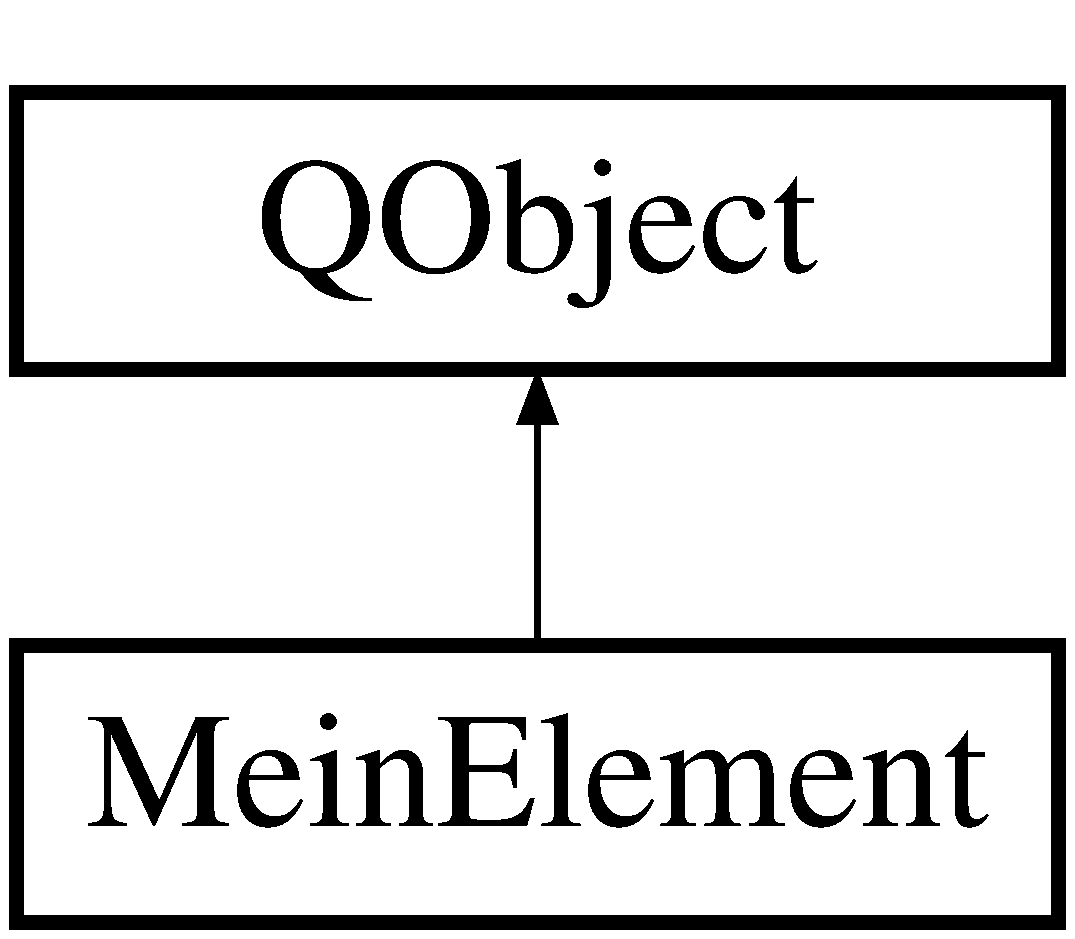
\includegraphics[height=2.000000cm]{class_mein_element}
\end{center}
\end{figure}
\subsection*{Public Member Functions}
\begin{DoxyCompactItemize}
\item 
\hyperlink{class_mein_element_a4a192d36a37deaaa20fb3aeefc7a2e12}{Mein\+Element} (b2\+World $\ast$world, Q\+Graphics\+Scene $\ast$level, b2\+Vec2 center, qreal length, qreal width, b2\+Body\+Type type, qreal friction)
\begin{DoxyCompactList}\small\item\em \hyperlink{class_mein_element_a4a192d36a37deaaa20fb3aeefc7a2e12}{Mein\+Element\+::\+Mein\+Element}. \end{DoxyCompactList}\item 
\hyperlink{class_mein_element_a0176c160758487042b6fca43d5141f8d}{Mein\+Element} (Q\+Graphics\+Scene $\ast$level, Q\+PointF center, qreal length, qreal width)
\begin{DoxyCompactList}\small\item\em \hyperlink{class_mein_element_a4a192d36a37deaaa20fb3aeefc7a2e12}{Mein\+Element\+::\+Mein\+Element}. \end{DoxyCompactList}\item 
void \hyperlink{class_mein_element_a711d5166f243d41f240990a3bf0bceff}{draw\+Bottom} ()
\end{DoxyCompactItemize}
\subsection*{Public Attributes}
\begin{DoxyCompactItemize}
\item 
b2\+Body $\ast$ \hyperlink{class_mein_element_a05117e05589fc0a4b1e144511fbd3eec}{body}
\begin{DoxyCompactList}\small\item\em Box2D Body of object. \end{DoxyCompactList}\item 
Q\+Graphics\+Item $\ast$ \hyperlink{class_mein_element_a6d0a318f2e37f3633f7cf6fc20e83531}{graphics}
\begin{DoxyCompactList}\small\item\em graphic of object \end{DoxyCompactList}\item 
Q\+Graphics\+Item $\ast$ \hyperlink{class_mein_element_a4811ea6a6c50dfad16c39bbaa9a758b8}{white}
\begin{DoxyCompactList}\small\item\em graphic of box, where \textquotesingle{}Finished\textquotesingle{} message is written. \end{DoxyCompactList}\item 
Q\+Media\+Player $\ast$ \hyperlink{class_mein_element_a04019be8ecb452cf4ee984efed24e9e1}{applause}
\begin{DoxyCompactList}\small\item\em Soundplayer for successfully finished level. \end{DoxyCompactList}\end{DoxyCompactItemize}


\subsection{Constructor \& Destructor Documentation}
\index{Mein\+Element@{Mein\+Element}!Mein\+Element@{Mein\+Element}}
\index{Mein\+Element@{Mein\+Element}!Mein\+Element@{Mein\+Element}}
\subsubsection[{\texorpdfstring{Mein\+Element(b2\+World $\ast$world, Q\+Graphics\+Scene $\ast$level, b2\+Vec2 center, qreal length, qreal width, b2\+Body\+Type type, qreal friction)}{MeinElement(b2World *world, QGraphicsScene *level, b2Vec2 center, qreal length, qreal width, b2BodyType type, qreal friction)}}]{\setlength{\rightskip}{0pt plus 5cm}Mein\+Element\+::\+Mein\+Element (
\begin{DoxyParamCaption}
\item[{b2\+World $\ast$}]{world, }
\item[{Q\+Graphics\+Scene $\ast$}]{level, }
\item[{b2\+Vec2}]{center, }
\item[{qreal}]{length, }
\item[{qreal}]{width, }
\item[{b2\+Body\+Type}]{type, }
\item[{qreal}]{friction}
\end{DoxyParamCaption}
)}\hypertarget{class_mein_element_a4a192d36a37deaaa20fb3aeefc7a2e12}{}\label{class_mein_element_a4a192d36a37deaaa20fb3aeefc7a2e12}


\hyperlink{class_mein_element_a4a192d36a37deaaa20fb3aeefc7a2e12}{Mein\+Element\+::\+Mein\+Element}. 


\begin{DoxyParams}{Parameters}
{\em world} & \+: Box2D world for physic engine \\
\hline
{\em level} & \+: Scene for the game \\
\hline
{\em center} & \+: center of the object \\
\hline
{\em length} & \+: length of the object \\
\hline
{\em width} & \+: Breite of the object \\
\hline
{\em type} & \+: Box2D type of the Bbock(if it\textquotesingle{}s static or dynamic) \\
\hline
{\em friction} & \+: friction for the \hyperlink{class_block}{Block} \\
\hline
\end{DoxyParams}
\index{Mein\+Element@{Mein\+Element}!Mein\+Element@{Mein\+Element}}
\index{Mein\+Element@{Mein\+Element}!Mein\+Element@{Mein\+Element}}
\subsubsection[{\texorpdfstring{Mein\+Element(\+Q\+Graphics\+Scene $\ast$level, Q\+Point\+F center, qreal length, qreal width)}{MeinElement(QGraphicsScene *level, QPointF center, qreal length, qreal width)}}]{\setlength{\rightskip}{0pt plus 5cm}Mein\+Element\+::\+Mein\+Element (
\begin{DoxyParamCaption}
\item[{Q\+Graphics\+Scene $\ast$}]{level, }
\item[{Q\+PointF}]{center, }
\item[{qreal}]{length, }
\item[{qreal}]{width}
\end{DoxyParamCaption}
)}\hypertarget{class_mein_element_a0176c160758487042b6fca43d5141f8d}{}\label{class_mein_element_a0176c160758487042b6fca43d5141f8d}


\hyperlink{class_mein_element_a4a192d36a37deaaa20fb3aeefc7a2e12}{Mein\+Element\+::\+Mein\+Element}. 


\begin{DoxyParams}{Parameters}
{\em level} & \+: Scene for the game \\
\hline
{\em center} & \+: Center of object (coordinates) \\
\hline
{\em length} & \+: length of object \\
\hline
{\em width} & \+: length of object Message Box Background for \textquotesingle{}Finished Level\textquotesingle{} \\
\hline
\end{DoxyParams}


\subsection{Member Function Documentation}
\index{Mein\+Element@{Mein\+Element}!draw\+Bottom@{draw\+Bottom}}
\index{draw\+Bottom@{draw\+Bottom}!Mein\+Element@{Mein\+Element}}
\subsubsection[{\texorpdfstring{draw\+Bottom()}{drawBottom()}}]{\setlength{\rightskip}{0pt plus 5cm}void Mein\+Element\+::draw\+Bottom (
\begin{DoxyParamCaption}
{}
\end{DoxyParamCaption}
)}\hypertarget{class_mein_element_a711d5166f243d41f240990a3bf0bceff}{}\label{class_mein_element_a711d5166f243d41f240990a3bf0bceff}


\subsection{Member Data Documentation}
\index{Mein\+Element@{Mein\+Element}!applause@{applause}}
\index{applause@{applause}!Mein\+Element@{Mein\+Element}}
\subsubsection[{\texorpdfstring{applause}{applause}}]{\setlength{\rightskip}{0pt plus 5cm}Q\+Media\+Player$\ast$ Mein\+Element\+::applause}\hypertarget{class_mein_element_a04019be8ecb452cf4ee984efed24e9e1}{}\label{class_mein_element_a04019be8ecb452cf4ee984efed24e9e1}


Soundplayer for successfully finished level. 

\index{Mein\+Element@{Mein\+Element}!body@{body}}
\index{body@{body}!Mein\+Element@{Mein\+Element}}
\subsubsection[{\texorpdfstring{body}{body}}]{\setlength{\rightskip}{0pt plus 5cm}b2\+Body$\ast$ Mein\+Element\+::body}\hypertarget{class_mein_element_a05117e05589fc0a4b1e144511fbd3eec}{}\label{class_mein_element_a05117e05589fc0a4b1e144511fbd3eec}


Box2D Body of object. 

\index{Mein\+Element@{Mein\+Element}!graphics@{graphics}}
\index{graphics@{graphics}!Mein\+Element@{Mein\+Element}}
\subsubsection[{\texorpdfstring{graphics}{graphics}}]{\setlength{\rightskip}{0pt plus 5cm}Q\+Graphics\+Item$\ast$ Mein\+Element\+::graphics}\hypertarget{class_mein_element_a6d0a318f2e37f3633f7cf6fc20e83531}{}\label{class_mein_element_a6d0a318f2e37f3633f7cf6fc20e83531}


graphic of object 

\index{Mein\+Element@{Mein\+Element}!white@{white}}
\index{white@{white}!Mein\+Element@{Mein\+Element}}
\subsubsection[{\texorpdfstring{white}{white}}]{\setlength{\rightskip}{0pt plus 5cm}Q\+Graphics\+Item$\ast$ Mein\+Element\+::white}\hypertarget{class_mein_element_a4811ea6a6c50dfad16c39bbaa9a758b8}{}\label{class_mein_element_a4811ea6a6c50dfad16c39bbaa9a758b8}


graphic of box, where \textquotesingle{}Finished\textquotesingle{} message is written. 



The documentation for this class was generated from the following files\+:\begin{DoxyCompactItemize}
\item 
Game/\hyperlink{meinelement_8h}{meinelement.\+h}\item 
Game/\hyperlink{meinelement_8cpp}{meinelement.\+cpp}\end{DoxyCompactItemize}

\hypertarget{class_mover}{}\section{Mover Class Reference}
\label{class_mover}\index{Mover@{Mover}}


{\ttfamily \#include $<$mover.\+h$>$}

\subsection*{Public Member Functions}
\begin{DoxyCompactItemize}
\item 
\hyperlink{class_mover_a8ec5e7ce87190ce9b25f1df64efa7821}{Mover} (b2\+World $\ast$world, Q\+Graphics\+Scene $\ast$level, b2\+Vec2 center, qreal m\+\_\+angle, qreal m\+\_\+length, qreal m\+\_\+width, qreal friction, Q\+String mode)
\begin{DoxyCompactList}\small\item\em \hyperlink{class_mover_a8ec5e7ce87190ce9b25f1df64efa7821}{Mover\+::\+Mover}. \end{DoxyCompactList}\end{DoxyCompactItemize}
\subsection*{Public Attributes}
\begin{DoxyCompactItemize}
\item 
qreal \hyperlink{class_mover_a2c55f3d5a807d328bcc8c73cdef5dda2}{length}
\item 
qreal \hyperlink{class_mover_ab78fbf587764d7cdcd417d2a444408d4}{width}
\item 
qreal \hyperlink{class_mover_acb7d779b2ce97a86149990dce48e88b5}{angle}
\item 
b2\+Body $\ast$ \hyperlink{class_mover_a6e91384098180f0fef918dd45f97f201}{body}
\item 
Q\+Graphics\+Item $\ast$ \hyperlink{class_mover_a111eebc06a95c11dc6f48dcc6a33478f}{graphics}
\end{DoxyCompactItemize}


\subsection{Constructor \& Destructor Documentation}
\index{Mover@{Mover}!Mover@{Mover}}
\index{Mover@{Mover}!Mover@{Mover}}
\subsubsection[{\texorpdfstring{Mover(b2\+World $\ast$world, Q\+Graphics\+Scene $\ast$level, b2\+Vec2 center, qreal m\+\_\+angle, qreal m\+\_\+length, qreal m\+\_\+width, qreal friction, Q\+String mode)}{Mover(b2World *world, QGraphicsScene *level, b2Vec2 center, qreal m_angle, qreal m_length, qreal m_width, qreal friction, QString mode)}}]{\setlength{\rightskip}{0pt plus 5cm}Mover\+::\+Mover (
\begin{DoxyParamCaption}
\item[{b2\+World $\ast$}]{world, }
\item[{Q\+Graphics\+Scene $\ast$}]{level, }
\item[{b2\+Vec2}]{center, }
\item[{qreal}]{m\+\_\+angle, }
\item[{qreal}]{m\+\_\+length, }
\item[{qreal}]{m\+\_\+width, }
\item[{qreal}]{friction, }
\item[{Q\+String}]{mode}
\end{DoxyParamCaption}
)}\hypertarget{class_mover_a8ec5e7ce87190ce9b25f1df64efa7821}{}\label{class_mover_a8ec5e7ce87190ce9b25f1df64efa7821}


\hyperlink{class_mover_a8ec5e7ce87190ce9b25f1df64efa7821}{Mover\+::\+Mover}. 


\begin{DoxyParams}{Parameters}
{\em world} & \\
\hline
{\em level} & \\
\hline
{\em center} & \\
\hline
{\em m\+\_\+angle} & \\
\hline
{\em m\+\_\+length} & \\
\hline
{\em m\+\_\+width} & \\
\hline
{\em type} & \\
\hline
{\em friction} & \\
\hline
{\em mode} & \\
\hline
\end{DoxyParams}


\subsection{Member Data Documentation}
\index{Mover@{Mover}!angle@{angle}}
\index{angle@{angle}!Mover@{Mover}}
\subsubsection[{\texorpdfstring{angle}{angle}}]{\setlength{\rightskip}{0pt plus 5cm}qreal Mover\+::angle}\hypertarget{class_mover_acb7d779b2ce97a86149990dce48e88b5}{}\label{class_mover_acb7d779b2ce97a86149990dce48e88b5}
\index{Mover@{Mover}!body@{body}}
\index{body@{body}!Mover@{Mover}}
\subsubsection[{\texorpdfstring{body}{body}}]{\setlength{\rightskip}{0pt plus 5cm}b2\+Body$\ast$ Mover\+::body}\hypertarget{class_mover_a6e91384098180f0fef918dd45f97f201}{}\label{class_mover_a6e91384098180f0fef918dd45f97f201}
\index{Mover@{Mover}!graphics@{graphics}}
\index{graphics@{graphics}!Mover@{Mover}}
\subsubsection[{\texorpdfstring{graphics}{graphics}}]{\setlength{\rightskip}{0pt plus 5cm}Q\+Graphics\+Item$\ast$ Mover\+::graphics}\hypertarget{class_mover_a111eebc06a95c11dc6f48dcc6a33478f}{}\label{class_mover_a111eebc06a95c11dc6f48dcc6a33478f}
\index{Mover@{Mover}!length@{length}}
\index{length@{length}!Mover@{Mover}}
\subsubsection[{\texorpdfstring{length}{length}}]{\setlength{\rightskip}{0pt plus 5cm}qreal Mover\+::length}\hypertarget{class_mover_a2c55f3d5a807d328bcc8c73cdef5dda2}{}\label{class_mover_a2c55f3d5a807d328bcc8c73cdef5dda2}
\index{Mover@{Mover}!width@{width}}
\index{width@{width}!Mover@{Mover}}
\subsubsection[{\texorpdfstring{width}{width}}]{\setlength{\rightskip}{0pt plus 5cm}qreal Mover\+::width}\hypertarget{class_mover_ab78fbf587764d7cdcd417d2a444408d4}{}\label{class_mover_ab78fbf587764d7cdcd417d2a444408d4}


The documentation for this class was generated from the following files\+:\begin{DoxyCompactItemize}
\item 
Game/\hyperlink{mover_8h}{mover.\+h}\item 
Game/\hyperlink{mover_8cpp}{mover.\+cpp}\end{DoxyCompactItemize}

\hypertarget{class_paperball}{}\section{Paperball Class Reference}
\label{class_paperball}\index{Paperball@{Paperball}}


The \hyperlink{class_paperball}{Paperball} class.  




{\ttfamily \#include $<$paperball.\+h$>$}

Inheritance diagram for Paperball\+:\begin{figure}[H]
\begin{center}
\leavevmode
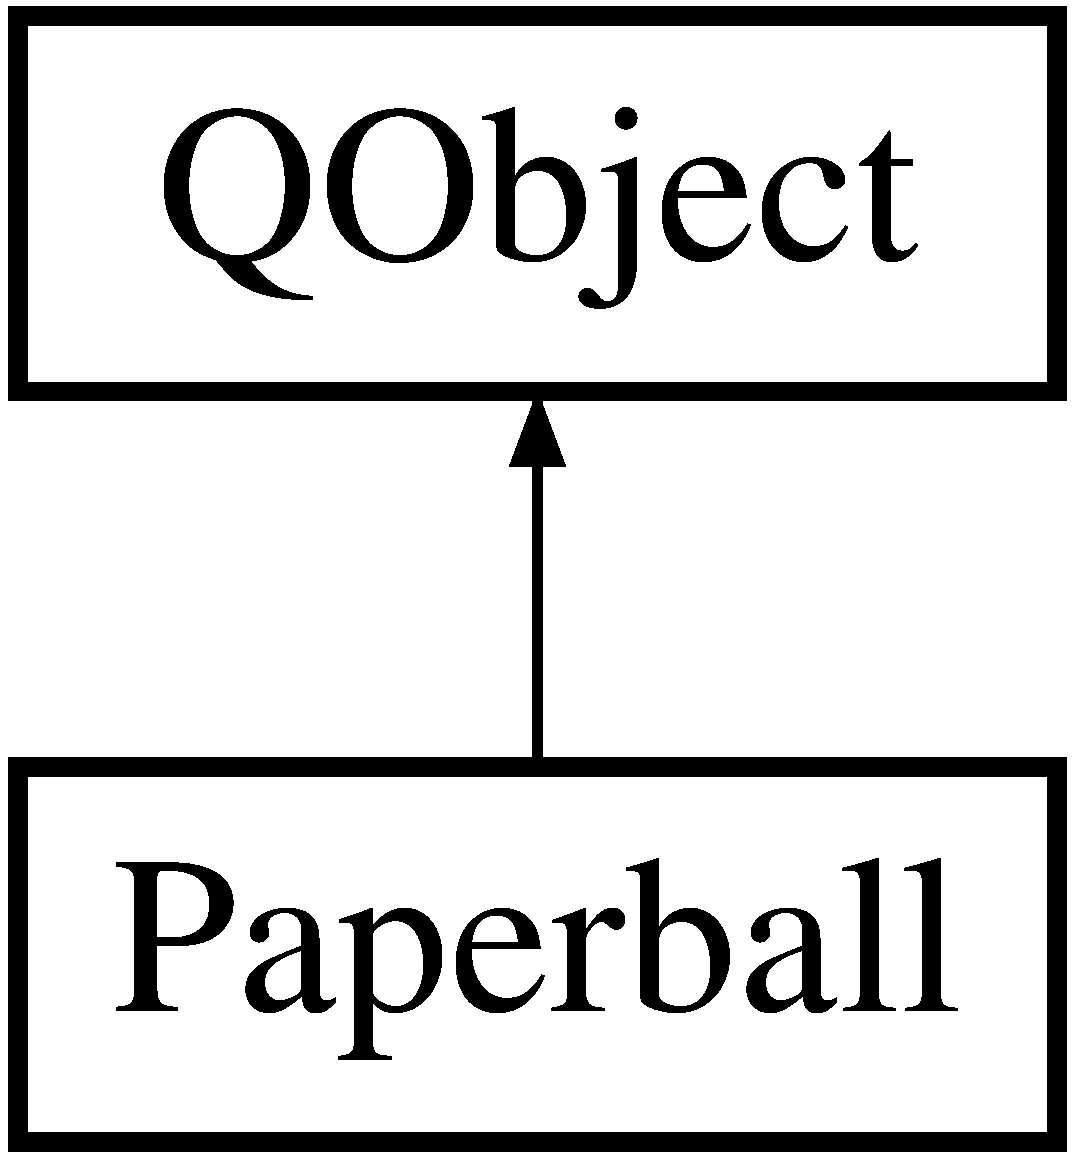
\includegraphics[height=2.000000cm]{class_paperball}
\end{center}
\end{figure}
\subsection*{Public Member Functions}
\begin{DoxyCompactItemize}
\item 
\hyperlink{class_paperball_ad0d9d4562bd894e529fdfa7a3ecb8e96}{Paperball} (b2\+World $\ast$world, Q\+Graphics\+Scene $\ast$level, Q\+PointF position, qreal angle, b2\+Body\+Type type, b2\+Circle\+Shape \&circle)
\begin{DoxyCompactList}\small\item\em \hyperlink{class_paperball_ad0d9d4562bd894e529fdfa7a3ecb8e96}{Paperball\+::\+Paperball}. \end{DoxyCompactList}\item 
void \hyperlink{class_paperball_a1d3b557c34068db1c78816c9147fe680}{create\+Paper} (b2\+World world, Q\+Graphics\+Scene levelscene, Q\+PointF pos, qreal angle, b2\+Body\+Type type, b2\+Circle\+Shape \&circle)
\item 
bool \hyperlink{class_paperball_a3bb15d3327d35c3408fe7e5b06bce078}{draw\+Ball1} ()
\begin{DoxyCompactList}\small\item\em \hyperlink{class_paperball_a3bb15d3327d35c3408fe7e5b06bce078}{Paperball\+::draw\+Ball1} connects the Graphics to the Box2\+D-\/\+Object checkout if paperball fell into the recyclebin. \end{DoxyCompactList}\end{DoxyCompactItemize}
\subsection*{Public Attributes}
\begin{DoxyCompactItemize}
\item 
b2\+Body $\ast$ \hyperlink{class_paperball_a5d5b3e0d4237ba80fe9590f49c88a0c0}{body}
\begin{DoxyCompactList}\small\item\em Box2D Body of Object. \end{DoxyCompactList}\item 
Q\+Graphics\+Item $\ast$ \hyperlink{class_paperball_a87b4515e298699c840f541ee637215dd}{graphics}
\begin{DoxyCompactList}\small\item\em Graphic of Object. \end{DoxyCompactList}\end{DoxyCompactItemize}


\subsection{Detailed Description}
The \hyperlink{class_paperball}{Paperball} class. 

\subsection{Constructor \& Destructor Documentation}
\index{Paperball@{Paperball}!Paperball@{Paperball}}
\index{Paperball@{Paperball}!Paperball@{Paperball}}
\subsubsection[{\texorpdfstring{Paperball(b2\+World $\ast$world, Q\+Graphics\+Scene $\ast$level, Q\+Point\+F position, qreal angle, b2\+Body\+Type type, b2\+Circle\+Shape \&circle)}{Paperball(b2World *world, QGraphicsScene *level, QPointF position, qreal angle, b2BodyType type, b2CircleShape &circle)}}]{\setlength{\rightskip}{0pt plus 5cm}Paperball\+::\+Paperball (
\begin{DoxyParamCaption}
\item[{b2\+World $\ast$}]{world, }
\item[{Q\+Graphics\+Scene $\ast$}]{level, }
\item[{Q\+PointF}]{position, }
\item[{qreal}]{angle, }
\item[{b2\+Body\+Type}]{type, }
\item[{b2\+Circle\+Shape \&}]{circle}
\end{DoxyParamCaption}
)}\hypertarget{class_paperball_ad0d9d4562bd894e529fdfa7a3ecb8e96}{}\label{class_paperball_ad0d9d4562bd894e529fdfa7a3ecb8e96}


\hyperlink{class_paperball_ad0d9d4562bd894e529fdfa7a3ecb8e96}{Paperball\+::\+Paperball}. 


\begin{DoxyParams}{Parameters}
{\em world} & \\
\hline
{\em level} & \\
\hline
{\em position} & \\
\hline
{\em angle} & \\
\hline
{\em type} & \\
\hline
{\em circle} & \\
\hline
\end{DoxyParams}


\subsection{Member Function Documentation}
\index{Paperball@{Paperball}!create\+Paper@{create\+Paper}}
\index{create\+Paper@{create\+Paper}!Paperball@{Paperball}}
\subsubsection[{\texorpdfstring{create\+Paper(b2\+World world, Q\+Graphics\+Scene levelscene, Q\+Point\+F pos, qreal angle, b2\+Body\+Type type, b2\+Circle\+Shape \&circle)}{createPaper(b2World world, QGraphicsScene levelscene, QPointF pos, qreal angle, b2BodyType type, b2CircleShape &circle)}}]{\setlength{\rightskip}{0pt plus 5cm}void Paperball\+::create\+Paper (
\begin{DoxyParamCaption}
\item[{b2\+World}]{world, }
\item[{Q\+Graphics\+Scene}]{levelscene, }
\item[{Q\+PointF}]{pos, }
\item[{qreal}]{angle, }
\item[{b2\+Body\+Type}]{type, }
\item[{b2\+Circle\+Shape \&}]{circle}
\end{DoxyParamCaption}
)}\hypertarget{class_paperball_a1d3b557c34068db1c78816c9147fe680}{}\label{class_paperball_a1d3b557c34068db1c78816c9147fe680}
\index{Paperball@{Paperball}!draw\+Ball1@{draw\+Ball1}}
\index{draw\+Ball1@{draw\+Ball1}!Paperball@{Paperball}}
\subsubsection[{\texorpdfstring{draw\+Ball1()}{drawBall1()}}]{\setlength{\rightskip}{0pt plus 5cm}bool Paperball\+::draw\+Ball1 (
\begin{DoxyParamCaption}
{}
\end{DoxyParamCaption}
)}\hypertarget{class_paperball_a3bb15d3327d35c3408fe7e5b06bce078}{}\label{class_paperball_a3bb15d3327d35c3408fe7e5b06bce078}


\hyperlink{class_paperball_a3bb15d3327d35c3408fe7e5b06bce078}{Paperball\+::draw\+Ball1} connects the Graphics to the Box2\+D-\/\+Object checkout if paperball fell into the recyclebin. 

\begin{DoxyReturn}{Returns}

\end{DoxyReturn}


\subsection{Member Data Documentation}
\index{Paperball@{Paperball}!body@{body}}
\index{body@{body}!Paperball@{Paperball}}
\subsubsection[{\texorpdfstring{body}{body}}]{\setlength{\rightskip}{0pt plus 5cm}b2\+Body$\ast$ Paperball\+::body}\hypertarget{class_paperball_a5d5b3e0d4237ba80fe9590f49c88a0c0}{}\label{class_paperball_a5d5b3e0d4237ba80fe9590f49c88a0c0}


Box2D Body of Object. 

\index{Paperball@{Paperball}!graphics@{graphics}}
\index{graphics@{graphics}!Paperball@{Paperball}}
\subsubsection[{\texorpdfstring{graphics}{graphics}}]{\setlength{\rightskip}{0pt plus 5cm}Q\+Graphics\+Item$\ast$ Paperball\+::graphics}\hypertarget{class_paperball_a87b4515e298699c840f541ee637215dd}{}\label{class_paperball_a87b4515e298699c840f541ee637215dd}


Graphic of Object. 



The documentation for this class was generated from the following files\+:\begin{DoxyCompactItemize}
\item 
C\+:/\+Users/\+Maximilian/\+Desktop/\+T\+U\+M/6.\+Semester/\+Grundkurs C++/\+Hauptprojekt/gruppe4\+\_\+hauptprojekt/gruppe4\+\_\+hauptprojekt/\+Game/\hyperlink{paperball_8h}{paperball.\+h}\item 
C\+:/\+Users/\+Maximilian/\+Desktop/\+T\+U\+M/6.\+Semester/\+Grundkurs C++/\+Hauptprojekt/gruppe4\+\_\+hauptprojekt/gruppe4\+\_\+hauptprojekt/\+Game/\hyperlink{paperball_8cpp}{paperball.\+cpp}\end{DoxyCompactItemize}

\hypertarget{classpic_button}{}\section{pic\+Button Class Reference}
\label{classpic_button}\index{pic\+Button@{pic\+Button}}


The \hyperlink{classpic_button}{pic\+Button} class.  




{\ttfamily \#include $<$picbutton.\+h$>$}

Inheritance diagram for pic\+Button\+:\begin{figure}[H]
\begin{center}
\leavevmode
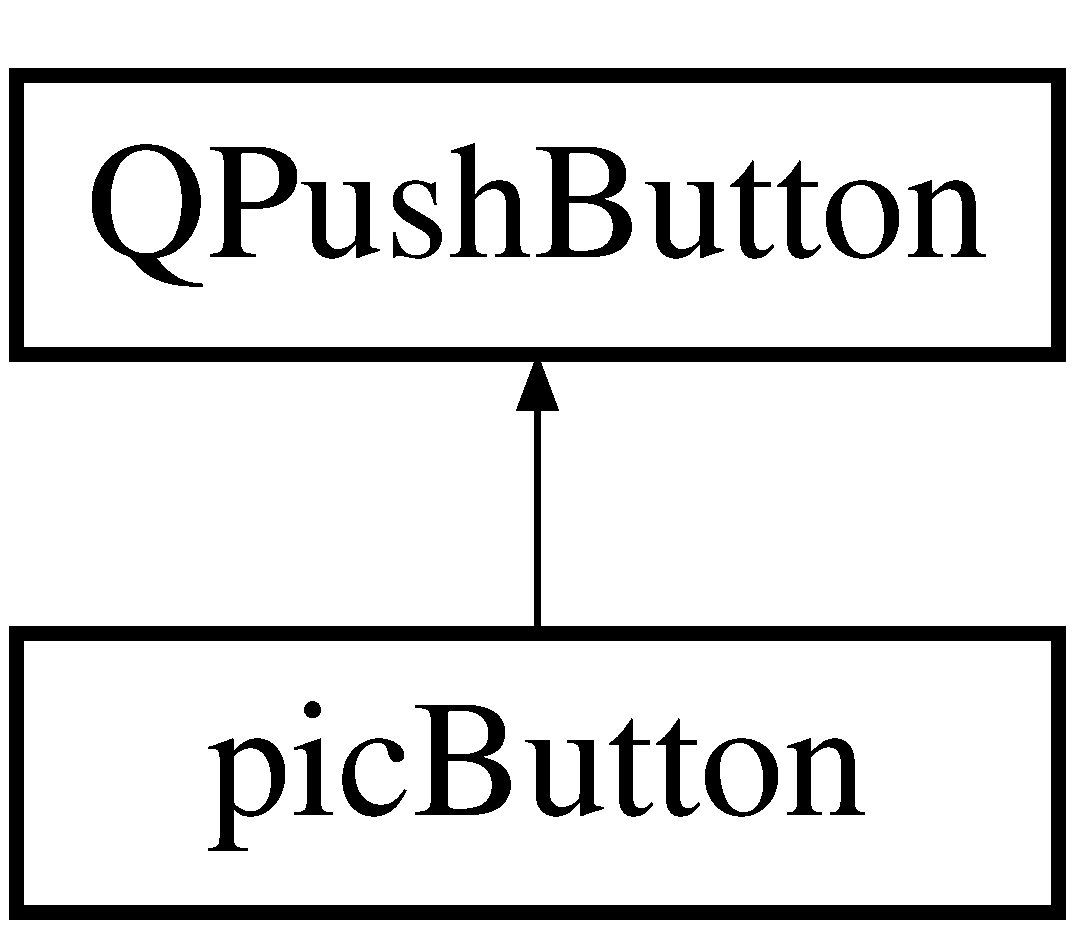
\includegraphics[height=2.000000cm]{classpic_button}
\end{center}
\end{figure}
\subsection*{Public Member Functions}
\begin{DoxyCompactItemize}
\item 
\hyperlink{classpic_button_a1d5dc5f3e6a73e24dd873fb6a33a3e7f}{pic\+Button} (Q\+Pixmap \+\_\+defaultpic, Q\+Pixmap \+\_\+hoverpic)
\begin{DoxyCompactList}\small\item\em \hyperlink{classpic_button_a1d5dc5f3e6a73e24dd873fb6a33a3e7f}{pic\+Button\+::pic\+Button} \end{DoxyCompactList}\item 
\hyperlink{classpic_button_a6c7eca4ea10251d19dde58edea0f0e12}{pic\+Button} (Q\+Pixmap \+\_\+defaultpic, Q\+Pixmap \+\_\+hoverpic, bool \hyperlink{classpic_button_ab011ab567cb14054023cc46cfc3110c1}{hover})
\begin{DoxyCompactList}\small\item\em \hyperlink{classpic_button_a1d5dc5f3e6a73e24dd873fb6a33a3e7f}{pic\+Button\+::pic\+Button} \end{DoxyCompactList}\item 
void \hyperlink{classpic_button_a8e06509469d6b2c5efe9c58558209350}{enter\+Event} (Q\+Event $\ast$event)
\begin{DoxyCompactList}\small\item\em \hyperlink{classpic_button_a8e06509469d6b2c5efe9c58558209350}{pic\+Button\+::enter\+Event} \end{DoxyCompactList}\item 
void \hyperlink{classpic_button_a22c110a8f610d4a315b2c260e7d1f2b9}{leave\+Event} (Q\+Event $\ast$event)
\begin{DoxyCompactList}\small\item\em \hyperlink{classpic_button_a22c110a8f610d4a315b2c260e7d1f2b9}{pic\+Button\+::leave\+Event} \end{DoxyCompactList}\item 
void \hyperlink{classpic_button_a38c0a41c10500e605cda766094ee00a5}{setdefaultpic} (Q\+Pixmap \hyperlink{classpic_button_a13f03c5d3c47b0a10b3798f9588a8cf5}{defaultpic})
\begin{DoxyCompactList}\small\item\em \hyperlink{classpic_button_a38c0a41c10500e605cda766094ee00a5}{pic\+Button\+::setdefaultpic} \end{DoxyCompactList}\item 
void \hyperlink{classpic_button_a632d61dedf5693fcade81c6a998a377d}{sethoverpic} (Q\+Pixmap \hyperlink{classpic_button_a6e387b9fc6348b681a786db8452fbc9d}{hoverpic})
\begin{DoxyCompactList}\small\item\em \hyperlink{classpic_button_a632d61dedf5693fcade81c6a998a377d}{pic\+Button\+::sethoverpic} \end{DoxyCompactList}\end{DoxyCompactItemize}
\subsection*{Public Attributes}
\begin{DoxyCompactItemize}
\item 
Q\+Pixmap \hyperlink{classpic_button_a13f03c5d3c47b0a10b3798f9588a8cf5}{defaultpic}
\begin{DoxyCompactList}\small\item\em Picture of Button. \end{DoxyCompactList}\item 
Q\+Pixmap \hyperlink{classpic_button_a6e387b9fc6348b681a786db8452fbc9d}{hoverpic}
\begin{DoxyCompactList}\small\item\em Picture when Button is selected. \end{DoxyCompactList}\item 
bool \hyperlink{classpic_button_ab011ab567cb14054023cc46cfc3110c1}{hover}
\end{DoxyCompactItemize}


\subsection{Detailed Description}
The \hyperlink{classpic_button}{pic\+Button} class. 

\subsection{Constructor \& Destructor Documentation}
\index{pic\+Button@{pic\+Button}!pic\+Button@{pic\+Button}}
\index{pic\+Button@{pic\+Button}!pic\+Button@{pic\+Button}}
\subsubsection[{\texorpdfstring{pic\+Button(\+Q\+Pixmap \+\_\+defaultpic, Q\+Pixmap \+\_\+hoverpic)}{picButton(QPixmap _defaultpic, QPixmap _hoverpic)}}]{\setlength{\rightskip}{0pt plus 5cm}pic\+Button\+::pic\+Button (
\begin{DoxyParamCaption}
\item[{Q\+Pixmap}]{\+\_\+defaultpic, }
\item[{Q\+Pixmap}]{\+\_\+hoverpic}
\end{DoxyParamCaption}
)}\hypertarget{classpic_button_a1d5dc5f3e6a73e24dd873fb6a33a3e7f}{}\label{classpic_button_a1d5dc5f3e6a73e24dd873fb6a33a3e7f}


\hyperlink{classpic_button_a1d5dc5f3e6a73e24dd873fb6a33a3e7f}{pic\+Button\+::pic\+Button} 


\begin{DoxyParams}{Parameters}
{\em \+\_\+defaultpic} & \\
\hline
{\em \+\_\+hoverpic} & \\
\hline
\end{DoxyParams}
Hovering mouse \index{pic\+Button@{pic\+Button}!pic\+Button@{pic\+Button}}
\index{pic\+Button@{pic\+Button}!pic\+Button@{pic\+Button}}
\subsubsection[{\texorpdfstring{pic\+Button(\+Q\+Pixmap \+\_\+defaultpic, Q\+Pixmap \+\_\+hoverpic, bool hover)}{picButton(QPixmap _defaultpic, QPixmap _hoverpic, bool hover)}}]{\setlength{\rightskip}{0pt plus 5cm}pic\+Button\+::pic\+Button (
\begin{DoxyParamCaption}
\item[{Q\+Pixmap}]{\+\_\+defaultpic, }
\item[{Q\+Pixmap}]{\+\_\+hoverpic, }
\item[{bool}]{\+\_\+hover}
\end{DoxyParamCaption}
)}\hypertarget{classpic_button_a6c7eca4ea10251d19dde58edea0f0e12}{}\label{classpic_button_a6c7eca4ea10251d19dde58edea0f0e12}


\hyperlink{classpic_button_a1d5dc5f3e6a73e24dd873fb6a33a3e7f}{pic\+Button\+::pic\+Button} 


\begin{DoxyParams}{Parameters}
{\em \+\_\+defaultpic} & picture of button \\
\hline
{\em \+\_\+hoverpic} & picture if you hover over button \\
\hline
{\em \+\_\+hover} & does mouse hover \\
\hline
\end{DoxyParams}
Hovering mouse 

\subsection{Member Function Documentation}
\index{pic\+Button@{pic\+Button}!enter\+Event@{enter\+Event}}
\index{enter\+Event@{enter\+Event}!pic\+Button@{pic\+Button}}
\subsubsection[{\texorpdfstring{enter\+Event(\+Q\+Event $\ast$event)}{enterEvent(QEvent *event)}}]{\setlength{\rightskip}{0pt plus 5cm}void pic\+Button\+::enter\+Event (
\begin{DoxyParamCaption}
\item[{Q\+Event $\ast$}]{event}
\end{DoxyParamCaption}
)}\hypertarget{classpic_button_a8e06509469d6b2c5efe9c58558209350}{}\label{classpic_button_a8e06509469d6b2c5efe9c58558209350}


\hyperlink{classpic_button_a8e06509469d6b2c5efe9c58558209350}{pic\+Button\+::enter\+Event} 


\begin{DoxyParams}{Parameters}
{\em event} & clickevent \\
\hline
\end{DoxyParams}
when hovering -\/$>$ change pic \index{pic\+Button@{pic\+Button}!leave\+Event@{leave\+Event}}
\index{leave\+Event@{leave\+Event}!pic\+Button@{pic\+Button}}
\subsubsection[{\texorpdfstring{leave\+Event(\+Q\+Event $\ast$event)}{leaveEvent(QEvent *event)}}]{\setlength{\rightskip}{0pt plus 5cm}void pic\+Button\+::leave\+Event (
\begin{DoxyParamCaption}
\item[{Q\+Event $\ast$}]{event}
\end{DoxyParamCaption}
)}\hypertarget{classpic_button_a22c110a8f610d4a315b2c260e7d1f2b9}{}\label{classpic_button_a22c110a8f610d4a315b2c260e7d1f2b9}


\hyperlink{classpic_button_a22c110a8f610d4a315b2c260e7d1f2b9}{pic\+Button\+::leave\+Event} 


\begin{DoxyParams}{Parameters}
{\em event} & mouse leave butto area \\
\hline
\end{DoxyParams}
Change pic back \index{pic\+Button@{pic\+Button}!setdefaultpic@{setdefaultpic}}
\index{setdefaultpic@{setdefaultpic}!pic\+Button@{pic\+Button}}
\subsubsection[{\texorpdfstring{setdefaultpic(\+Q\+Pixmap defaultpic)}{setdefaultpic(QPixmap defaultpic)}}]{\setlength{\rightskip}{0pt plus 5cm}void pic\+Button\+::setdefaultpic (
\begin{DoxyParamCaption}
\item[{Q\+Pixmap}]{\+\_\+defaultpic}
\end{DoxyParamCaption}
)}\hypertarget{classpic_button_a38c0a41c10500e605cda766094ee00a5}{}\label{classpic_button_a38c0a41c10500e605cda766094ee00a5}


\hyperlink{classpic_button_a38c0a41c10500e605cda766094ee00a5}{pic\+Button\+::setdefaultpic} 


\begin{DoxyParams}{Parameters}
{\em \+\_\+defaultpic} & insert picutre \\
\hline
\end{DoxyParams}
\index{pic\+Button@{pic\+Button}!sethoverpic@{sethoverpic}}
\index{sethoverpic@{sethoverpic}!pic\+Button@{pic\+Button}}
\subsubsection[{\texorpdfstring{sethoverpic(\+Q\+Pixmap hoverpic)}{sethoverpic(QPixmap hoverpic)}}]{\setlength{\rightskip}{0pt plus 5cm}void pic\+Button\+::sethoverpic (
\begin{DoxyParamCaption}
\item[{Q\+Pixmap}]{\+\_\+hoverpic}
\end{DoxyParamCaption}
)}\hypertarget{classpic_button_a632d61dedf5693fcade81c6a998a377d}{}\label{classpic_button_a632d61dedf5693fcade81c6a998a377d}


\hyperlink{classpic_button_a632d61dedf5693fcade81c6a998a377d}{pic\+Button\+::sethoverpic} 


\begin{DoxyParams}{Parameters}
{\em \+\_\+hoverpic} & insert picture \\
\hline
\end{DoxyParams}


\subsection{Member Data Documentation}
\index{pic\+Button@{pic\+Button}!defaultpic@{defaultpic}}
\index{defaultpic@{defaultpic}!pic\+Button@{pic\+Button}}
\subsubsection[{\texorpdfstring{defaultpic}{defaultpic}}]{\setlength{\rightskip}{0pt plus 5cm}Q\+Pixmap pic\+Button\+::defaultpic}\hypertarget{classpic_button_a13f03c5d3c47b0a10b3798f9588a8cf5}{}\label{classpic_button_a13f03c5d3c47b0a10b3798f9588a8cf5}


Picture of Button. 

\index{pic\+Button@{pic\+Button}!hover@{hover}}
\index{hover@{hover}!pic\+Button@{pic\+Button}}
\subsubsection[{\texorpdfstring{hover}{hover}}]{\setlength{\rightskip}{0pt plus 5cm}bool pic\+Button\+::hover}\hypertarget{classpic_button_ab011ab567cb14054023cc46cfc3110c1}{}\label{classpic_button_ab011ab567cb14054023cc46cfc3110c1}
\index{pic\+Button@{pic\+Button}!hoverpic@{hoverpic}}
\index{hoverpic@{hoverpic}!pic\+Button@{pic\+Button}}
\subsubsection[{\texorpdfstring{hoverpic}{hoverpic}}]{\setlength{\rightskip}{0pt plus 5cm}Q\+Pixmap pic\+Button\+::hoverpic}\hypertarget{classpic_button_a6e387b9fc6348b681a786db8452fbc9d}{}\label{classpic_button_a6e387b9fc6348b681a786db8452fbc9d}


Picture when Button is selected. 



The documentation for this class was generated from the following files\+:\begin{DoxyCompactItemize}
\item 
C\+:/\+Users/\+Maximilian/\+Desktop/\+T\+U\+M/6.\+Semester/\+Grundkurs C++/\+Hauptprojekt/gruppe4\+\_\+hauptprojekt/gruppe4\+\_\+hauptprojekt/\+Game/\hyperlink{picbutton_8h}{picbutton.\+h}\item 
C\+:/\+Users/\+Maximilian/\+Desktop/\+T\+U\+M/6.\+Semester/\+Grundkurs C++/\+Hauptprojekt/gruppe4\+\_\+hauptprojekt/gruppe4\+\_\+hauptprojekt/\+Game/\hyperlink{picbutton_8cpp}{picbutton.\+cpp}\end{DoxyCompactItemize}

\hypertarget{class_recycle_bin}{}\section{Recycle\+Bin Class Reference}
\label{class_recycle_bin}\index{Recycle\+Bin@{Recycle\+Bin}}


{\ttfamily \#include $<$recyclebin.\+h$>$}

\subsection*{Public Member Functions}
\begin{DoxyCompactItemize}
\item 
\hyperlink{class_recycle_bin_aff0bd5474a5d05939b234d1d951e86e8}{Recycle\+Bin} (b2\+World $\ast$world, Q\+Graphics\+Scene $\ast$level, Q\+PointF a, Q\+PointF b, Q\+PointF c, Q\+PointF d, qreal angle, b2\+Body\+Type type)
\begin{DoxyCompactList}\small\item\em \hyperlink{class_recycle_bin_aff0bd5474a5d05939b234d1d951e86e8}{Recycle\+Bin\+::\+Recycle\+Bin}. \end{DoxyCompactList}\item 
void \hyperlink{class_recycle_bin_ab8158c4e18c16fb3e55638a60327d978}{draw\+Graphics} ()
\begin{DoxyCompactList}\small\item\em \hyperlink{class_recycle_bin_ab8158c4e18c16fb3e55638a60327d978}{Recycle\+Bin\+::draw\+Graphics} connects the Box2\+D-\/\+Object to the Graphics after relocation. \end{DoxyCompactList}\end{DoxyCompactItemize}
\subsection*{Public Attributes}
\begin{DoxyCompactItemize}
\item 
b2\+Body $\ast$ \hyperlink{class_recycle_bin_a1e0b25e04920ce7dc737549928d1f45a}{body}
\item 
Q\+Graphics\+Item $\ast$ \hyperlink{class_recycle_bin_a876a38f5ba7524bd618c1c3749bb7a83}{graphics}
\end{DoxyCompactItemize}


\subsection{Detailed Description}


Definition at line 9 of file recyclebin.\+h.



\subsection{Constructor \& Destructor Documentation}
\index{Recycle\+Bin@{Recycle\+Bin}!Recycle\+Bin@{Recycle\+Bin}}
\index{Recycle\+Bin@{Recycle\+Bin}!Recycle\+Bin@{Recycle\+Bin}}
\subsubsection[{\texorpdfstring{Recycle\+Bin(b2\+World $\ast$world, Q\+Graphics\+Scene $\ast$level, Q\+Point\+F a, Q\+Point\+F b, Q\+Point\+F c, Q\+Point\+F d, qreal angle, b2\+Body\+Type type)}{RecycleBin(b2World *world, QGraphicsScene *level, QPointF a, QPointF b, QPointF c, QPointF d, qreal angle, b2BodyType type)}}]{\setlength{\rightskip}{0pt plus 5cm}Recycle\+Bin\+::\+Recycle\+Bin (
\begin{DoxyParamCaption}
\item[{b2\+World $\ast$}]{world, }
\item[{Q\+Graphics\+Scene $\ast$}]{level, }
\item[{Q\+PointF}]{a, }
\item[{Q\+PointF}]{b, }
\item[{Q\+PointF}]{c, }
\item[{Q\+PointF}]{d, }
\item[{qreal}]{angle, }
\item[{b2\+Body\+Type}]{type}
\end{DoxyParamCaption}
)}\hypertarget{class_recycle_bin_aff0bd5474a5d05939b234d1d951e86e8}{}\label{class_recycle_bin_aff0bd5474a5d05939b234d1d951e86e8}


\hyperlink{class_recycle_bin_aff0bd5474a5d05939b234d1d951e86e8}{Recycle\+Bin\+::\+Recycle\+Bin}. 


\begin{DoxyParams}{Parameters}
{\em world} & \\
\hline
{\em level} & \\
\hline
{\em a} & \\
\hline
{\em b} & \\
\hline
{\em c} & \\
\hline
{\em d} & \\
\hline
{\em angle} & \\
\hline
{\em type} & \\
\hline
\end{DoxyParams}


Definition at line 18 of file recyclebin.\+cpp.



\subsection{Member Function Documentation}
\index{Recycle\+Bin@{Recycle\+Bin}!draw\+Graphics@{draw\+Graphics}}
\index{draw\+Graphics@{draw\+Graphics}!Recycle\+Bin@{Recycle\+Bin}}
\subsubsection[{\texorpdfstring{draw\+Graphics()}{drawGraphics()}}]{\setlength{\rightskip}{0pt plus 5cm}void Recycle\+Bin\+::draw\+Graphics (
\begin{DoxyParamCaption}
{}
\end{DoxyParamCaption}
)}\hypertarget{class_recycle_bin_ab8158c4e18c16fb3e55638a60327d978}{}\label{class_recycle_bin_ab8158c4e18c16fb3e55638a60327d978}


\hyperlink{class_recycle_bin_ab8158c4e18c16fb3e55638a60327d978}{Recycle\+Bin\+::draw\+Graphics} connects the Box2\+D-\/\+Object to the Graphics after relocation. 



Definition at line 60 of file recyclebin.\+cpp.



\subsection{Member Data Documentation}
\index{Recycle\+Bin@{Recycle\+Bin}!body@{body}}
\index{body@{body}!Recycle\+Bin@{Recycle\+Bin}}
\subsubsection[{\texorpdfstring{body}{body}}]{\setlength{\rightskip}{0pt plus 5cm}b2\+Body$\ast$ Recycle\+Bin\+::body}\hypertarget{class_recycle_bin_a1e0b25e04920ce7dc737549928d1f45a}{}\label{class_recycle_bin_a1e0b25e04920ce7dc737549928d1f45a}


Definition at line 16 of file recyclebin.\+h.

\index{Recycle\+Bin@{Recycle\+Bin}!graphics@{graphics}}
\index{graphics@{graphics}!Recycle\+Bin@{Recycle\+Bin}}
\subsubsection[{\texorpdfstring{graphics}{graphics}}]{\setlength{\rightskip}{0pt plus 5cm}Q\+Graphics\+Item$\ast$ Recycle\+Bin\+::graphics}\hypertarget{class_recycle_bin_a876a38f5ba7524bd618c1c3749bb7a83}{}\label{class_recycle_bin_a876a38f5ba7524bd618c1c3749bb7a83}


Definition at line 17 of file recyclebin.\+h.



The documentation for this class was generated from the following files\+:\begin{DoxyCompactItemize}
\item 
C\+:/\+Users/\+Maximilian/\+Desktop/\+T\+U\+M/6.\+Semester/\+Grundkurs C++/\+Hauptprojekt/gruppe4\+\_\+hauptprojekt/gruppe4\+\_\+hauptprojekt/\+Game/\hyperlink{recyclebin_8h}{recyclebin.\+h}\item 
C\+:/\+Users/\+Maximilian/\+Desktop/\+T\+U\+M/6.\+Semester/\+Grundkurs C++/\+Hauptprojekt/gruppe4\+\_\+hauptprojekt/gruppe4\+\_\+hauptprojekt/\+Game/\hyperlink{recyclebin_8cpp}{recyclebin.\+cpp}\end{DoxyCompactItemize}

\hypertarget{class_recycle_bin_graphics}{}\section{Recycle\+Bin\+Graphics Class Reference}
\label{class_recycle_bin_graphics}\index{Recycle\+Bin\+Graphics@{Recycle\+Bin\+Graphics}}


{\ttfamily \#include $<$recyclebingraphics.\+h$>$}

\subsection*{Public Member Functions}
\begin{DoxyCompactItemize}
\item 
\hyperlink{class_recycle_bin_graphics_afe8714eec166ad6a723d382f60beaa74}{Recycle\+Bin\+Graphics} (Q\+Graphics\+Scene $\ast$level)
\begin{DoxyCompactList}\small\item\em \hyperlink{class_recycle_bin_graphics_afe8714eec166ad6a723d382f60beaa74}{Recycle\+Bin\+Graphics\+::\+Recycle\+Bin\+Graphics}. \end{DoxyCompactList}\end{DoxyCompactItemize}
\subsection*{Public Attributes}
\begin{DoxyCompactItemize}
\item 
Q\+Graphics\+Item $\ast$ \hyperlink{class_recycle_bin_graphics_af2e892576d357f795b21027c55557570}{graphics}
\end{DoxyCompactItemize}


\subsection{Detailed Description}


Definition at line 9 of file recyclebingraphics.\+h.



\subsection{Constructor \& Destructor Documentation}
\index{Recycle\+Bin\+Graphics@{Recycle\+Bin\+Graphics}!Recycle\+Bin\+Graphics@{Recycle\+Bin\+Graphics}}
\index{Recycle\+Bin\+Graphics@{Recycle\+Bin\+Graphics}!Recycle\+Bin\+Graphics@{Recycle\+Bin\+Graphics}}
\subsubsection[{\texorpdfstring{Recycle\+Bin\+Graphics(\+Q\+Graphics\+Scene $\ast$level)}{RecycleBinGraphics(QGraphicsScene *level)}}]{\setlength{\rightskip}{0pt plus 5cm}Recycle\+Bin\+Graphics\+::\+Recycle\+Bin\+Graphics (
\begin{DoxyParamCaption}
\item[{Q\+Graphics\+Scene $\ast$}]{level}
\end{DoxyParamCaption}
)}\hypertarget{class_recycle_bin_graphics_afe8714eec166ad6a723d382f60beaa74}{}\label{class_recycle_bin_graphics_afe8714eec166ad6a723d382f60beaa74}


\hyperlink{class_recycle_bin_graphics_afe8714eec166ad6a723d382f60beaa74}{Recycle\+Bin\+Graphics\+::\+Recycle\+Bin\+Graphics}. 


\begin{DoxyParams}{Parameters}
{\em level} & \\
\hline
\end{DoxyParams}


Definition at line 11 of file recyclebingraphics.\+cpp.



\subsection{Member Data Documentation}
\index{Recycle\+Bin\+Graphics@{Recycle\+Bin\+Graphics}!graphics@{graphics}}
\index{graphics@{graphics}!Recycle\+Bin\+Graphics@{Recycle\+Bin\+Graphics}}
\subsubsection[{\texorpdfstring{graphics}{graphics}}]{\setlength{\rightskip}{0pt plus 5cm}Q\+Graphics\+Item$\ast$ Recycle\+Bin\+Graphics\+::graphics}\hypertarget{class_recycle_bin_graphics_af2e892576d357f795b21027c55557570}{}\label{class_recycle_bin_graphics_af2e892576d357f795b21027c55557570}


Definition at line 14 of file recyclebingraphics.\+h.



The documentation for this class was generated from the following files\+:\begin{DoxyCompactItemize}
\item 
C\+:/\+Users/\+Maximilian/\+Desktop/\+T\+U\+M/6.\+Semester/\+Grundkurs C++/\+Hauptprojekt/gruppe4\+\_\+hauptprojekt/gruppe4\+\_\+hauptprojekt/\+Game/\hyperlink{recyclebingraphics_8h}{recyclebingraphics.\+h}\item 
C\+:/\+Users/\+Maximilian/\+Desktop/\+T\+U\+M/6.\+Semester/\+Grundkurs C++/\+Hauptprojekt/gruppe4\+\_\+hauptprojekt/gruppe4\+\_\+hauptprojekt/\+Game/\hyperlink{recyclebingraphics_8cpp}{recyclebingraphics.\+cpp}\end{DoxyCompactItemize}

\hypertarget{class_trampoline}{}\section{Trampoline Class Reference}
\label{class_trampoline}\index{Trampoline@{Trampoline}}


{\ttfamily \#include $<$trampoline.\+h$>$}

Inheritance diagram for Trampoline\+:\begin{figure}[H]
\begin{center}
\leavevmode
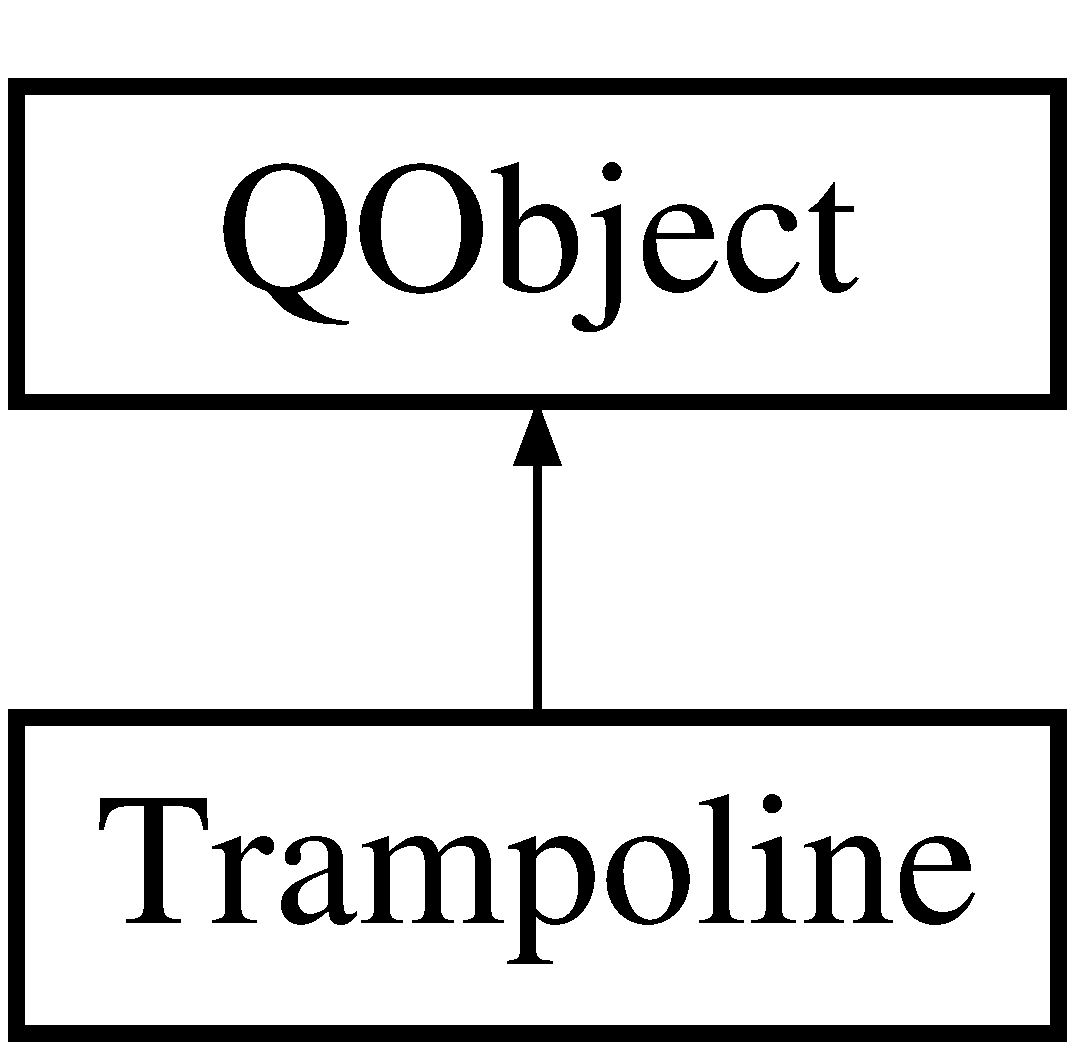
\includegraphics[height=2.000000cm]{class_trampoline}
\end{center}
\end{figure}
\subsection*{Public Member Functions}
\begin{DoxyCompactItemize}
\item 
\hyperlink{class_trampoline_a7f77638c6896a68464545bf3373df32b}{Trampoline} (b2\+World $\ast$world, Q\+Graphics\+Scene $\ast$level, b2\+Vec2 center, qreal m\+\_\+angle, qreal m\+\_\+length, qreal m\+\_\+width, b2\+Body\+Type type, qreal friction, Q\+String mode)
\begin{DoxyCompactList}\small\item\em \hyperlink{class_trampoline_a7f77638c6896a68464545bf3373df32b}{Trampoline\+::\+Trampoline}. \end{DoxyCompactList}\end{DoxyCompactItemize}
\subsection*{Public Attributes}
\begin{DoxyCompactItemize}
\item 
qreal \hyperlink{class_trampoline_afc20b8e85af09d551c0278b2dcc1d35d}{length}
\begin{DoxyCompactList}\small\item\em length of object \end{DoxyCompactList}\item 
qreal \hyperlink{class_trampoline_abc6d02536d9caeb1c1d80c545ebae044}{width}
\begin{DoxyCompactList}\small\item\em width of object \end{DoxyCompactList}\item 
qreal \hyperlink{class_trampoline_ae2b2f0ba18c591bbcf360f368758edf7}{angle}
\begin{DoxyCompactList}\small\item\em angle of object \end{DoxyCompactList}\item 
b2\+Body $\ast$ \hyperlink{class_trampoline_a5640097c2fa1b82b69338e3e3d5fc18e}{body}
\begin{DoxyCompactList}\small\item\em body of object \end{DoxyCompactList}\item 
Q\+Graphics\+Item $\ast$ \hyperlink{class_trampoline_a889e4c0143c14b47dc7575395356560a}{graphics}
\begin{DoxyCompactList}\small\item\em graphics of object \end{DoxyCompactList}\end{DoxyCompactItemize}


\subsection{Constructor \& Destructor Documentation}
\index{Trampoline@{Trampoline}!Trampoline@{Trampoline}}
\index{Trampoline@{Trampoline}!Trampoline@{Trampoline}}
\subsubsection[{\texorpdfstring{Trampoline(b2\+World $\ast$world, Q\+Graphics\+Scene $\ast$level, b2\+Vec2 center, qreal m\+\_\+angle, qreal m\+\_\+length, qreal m\+\_\+width, b2\+Body\+Type type, qreal friction, Q\+String mode)}{Trampoline(b2World *world, QGraphicsScene *level, b2Vec2 center, qreal m_angle, qreal m_length, qreal m_width, b2BodyType type, qreal friction, QString mode)}}]{\setlength{\rightskip}{0pt plus 5cm}Trampoline\+::\+Trampoline (
\begin{DoxyParamCaption}
\item[{b2\+World $\ast$}]{world, }
\item[{Q\+Graphics\+Scene $\ast$}]{level, }
\item[{b2\+Vec2}]{center, }
\item[{qreal}]{m\+\_\+angle, }
\item[{qreal}]{m\+\_\+length, }
\item[{qreal}]{m\+\_\+width, }
\item[{b2\+Body\+Type}]{type, }
\item[{qreal}]{friction, }
\item[{Q\+String}]{mode}
\end{DoxyParamCaption}
)}\hypertarget{class_trampoline_a7f77638c6896a68464545bf3373df32b}{}\label{class_trampoline_a7f77638c6896a68464545bf3373df32b}


\hyperlink{class_trampoline_a7f77638c6896a68464545bf3373df32b}{Trampoline\+::\+Trampoline}. 


\begin{DoxyParams}{Parameters}
{\em world} & \\
\hline
{\em level} & \\
\hline
{\em center} & \\
\hline
{\em m\+\_\+angle} & \\
\hline
{\em m\+\_\+length} & \\
\hline
{\em m\+\_\+width} & \\
\hline
{\em type} & \\
\hline
{\em friction} & \\
\hline
{\em mode} & \\
\hline
\end{DoxyParams}


\subsection{Member Data Documentation}
\index{Trampoline@{Trampoline}!angle@{angle}}
\index{angle@{angle}!Trampoline@{Trampoline}}
\subsubsection[{\texorpdfstring{angle}{angle}}]{\setlength{\rightskip}{0pt plus 5cm}qreal Trampoline\+::angle}\hypertarget{class_trampoline_ae2b2f0ba18c591bbcf360f368758edf7}{}\label{class_trampoline_ae2b2f0ba18c591bbcf360f368758edf7}


angle of object 

\index{Trampoline@{Trampoline}!body@{body}}
\index{body@{body}!Trampoline@{Trampoline}}
\subsubsection[{\texorpdfstring{body}{body}}]{\setlength{\rightskip}{0pt plus 5cm}b2\+Body$\ast$ Trampoline\+::body}\hypertarget{class_trampoline_a5640097c2fa1b82b69338e3e3d5fc18e}{}\label{class_trampoline_a5640097c2fa1b82b69338e3e3d5fc18e}


body of object 

\index{Trampoline@{Trampoline}!graphics@{graphics}}
\index{graphics@{graphics}!Trampoline@{Trampoline}}
\subsubsection[{\texorpdfstring{graphics}{graphics}}]{\setlength{\rightskip}{0pt plus 5cm}Q\+Graphics\+Item$\ast$ Trampoline\+::graphics}\hypertarget{class_trampoline_a889e4c0143c14b47dc7575395356560a}{}\label{class_trampoline_a889e4c0143c14b47dc7575395356560a}


graphics of object 

\index{Trampoline@{Trampoline}!length@{length}}
\index{length@{length}!Trampoline@{Trampoline}}
\subsubsection[{\texorpdfstring{length}{length}}]{\setlength{\rightskip}{0pt plus 5cm}qreal Trampoline\+::length}\hypertarget{class_trampoline_afc20b8e85af09d551c0278b2dcc1d35d}{}\label{class_trampoline_afc20b8e85af09d551c0278b2dcc1d35d}


length of object 

\index{Trampoline@{Trampoline}!width@{width}}
\index{width@{width}!Trampoline@{Trampoline}}
\subsubsection[{\texorpdfstring{width}{width}}]{\setlength{\rightskip}{0pt plus 5cm}qreal Trampoline\+::width}\hypertarget{class_trampoline_abc6d02536d9caeb1c1d80c545ebae044}{}\label{class_trampoline_abc6d02536d9caeb1c1d80c545ebae044}


width of object 



The documentation for this class was generated from the following files\+:\begin{DoxyCompactItemize}
\item 
C\+:/\+Users/\+Maximilian/\+Desktop/\+T\+U\+M/6.\+Semester/\+Grundkurs C++/\+Hauptprojekt/gruppe4\+\_\+hauptprojekt/gruppe4\+\_\+hauptprojekt/\+Game/\hyperlink{trampoline_8h}{trampoline.\+h}\item 
C\+:/\+Users/\+Maximilian/\+Desktop/\+T\+U\+M/6.\+Semester/\+Grundkurs C++/\+Hauptprojekt/gruppe4\+\_\+hauptprojekt/gruppe4\+\_\+hauptprojekt/\+Game/\hyperlink{trampoline_8cpp}{trampoline.\+cpp}\end{DoxyCompactItemize}

\hypertarget{class_triangle}{}\section{Triangle Class Reference}
\label{class_triangle}\index{Triangle@{Triangle}}


{\ttfamily \#include $<$triangle.\+h$>$}

Inheritance diagram for Triangle\+:\begin{figure}[H]
\begin{center}
\leavevmode
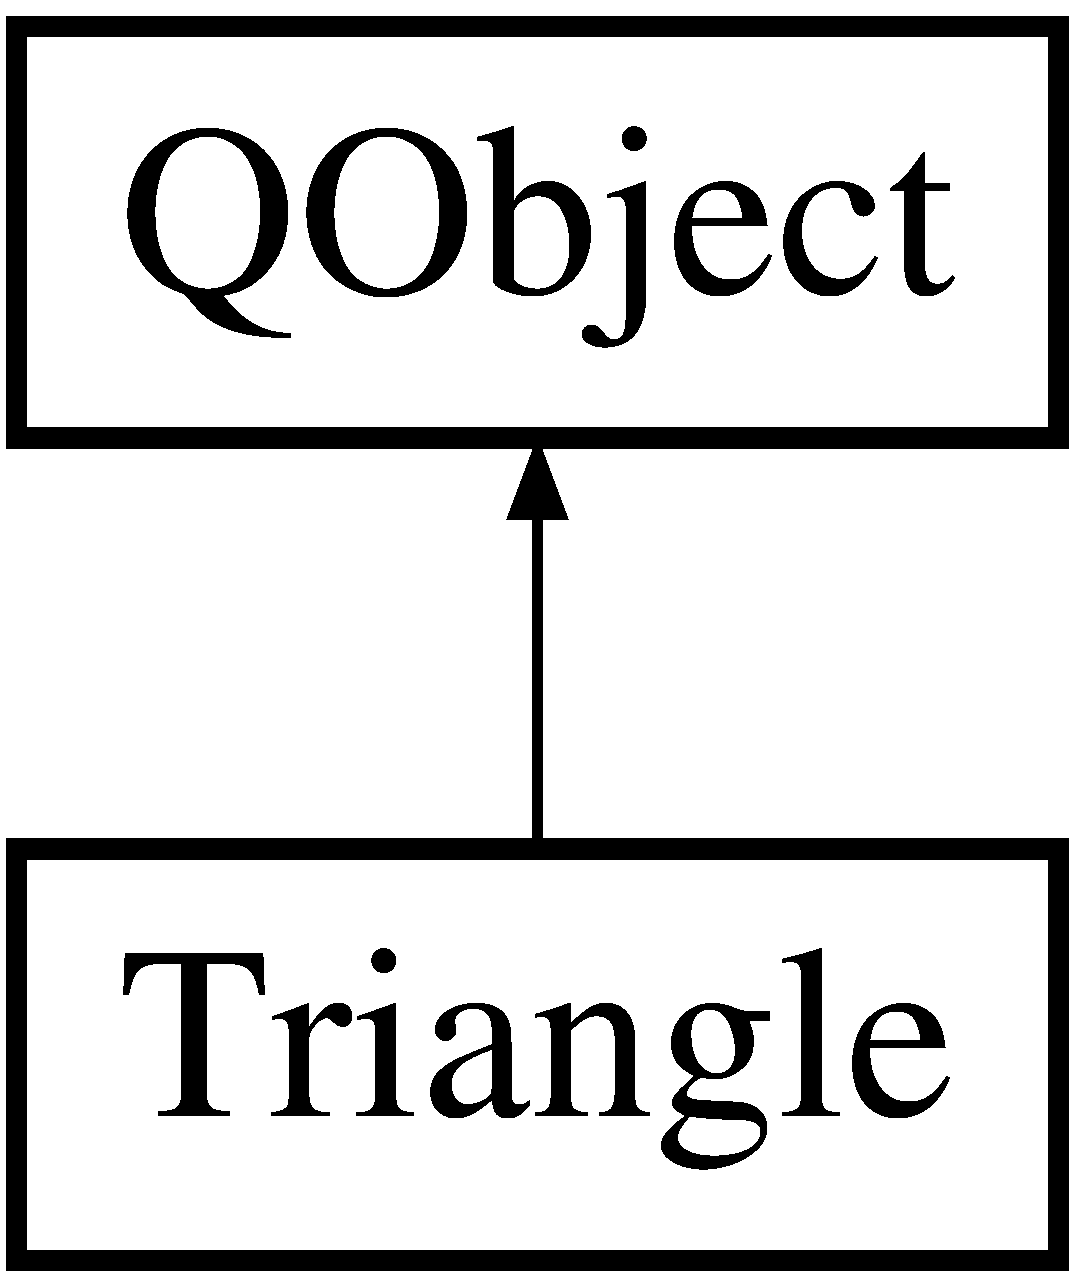
\includegraphics[height=2.000000cm]{class_triangle}
\end{center}
\end{figure}
\subsection*{Public Member Functions}
\begin{DoxyCompactItemize}
\item 
\hyperlink{class_triangle_a47f2b3f39a014d432f7a42d84f443370}{Triangle} (b2\+World $\ast$world, Q\+Graphics\+Scene $\ast$level, Q\+PointF a, Q\+PointF b, Q\+PointF c, qreal angle, b2\+Body\+Type type, qreal friction, Q\+String mode)
\begin{DoxyCompactList}\small\item\em \hyperlink{class_triangle_a47f2b3f39a014d432f7a42d84f443370}{Triangle\+::\+Triangle}. \end{DoxyCompactList}\item 
void \hyperlink{class_triangle_a37c8163fef65a3979e7cc8b076db936c}{draw\+Graphics} ()
\begin{DoxyCompactList}\small\item\em \hyperlink{class_triangle_a37c8163fef65a3979e7cc8b076db936c}{Triangle\+::draw\+Graphics} connects the Box2\+D-\/\+Object to the Graphics after relocation. \end{DoxyCompactList}\end{DoxyCompactItemize}
\subsection*{Public Attributes}
\begin{DoxyCompactItemize}
\item 
b2\+Body $\ast$ \hyperlink{class_triangle_a342320abc2a212d7f6a86a262ac438b6}{body}
\begin{DoxyCompactList}\small\item\em body of triangle \end{DoxyCompactList}\item 
Q\+Graphics\+Item $\ast$ \hyperlink{class_triangle_a914fac6f6bdac1dd191f82f5a5443646}{graphics}
\begin{DoxyCompactList}\small\item\em graphic of triangle \end{DoxyCompactList}\end{DoxyCompactItemize}


\subsection{Constructor \& Destructor Documentation}
\index{Triangle@{Triangle}!Triangle@{Triangle}}
\index{Triangle@{Triangle}!Triangle@{Triangle}}
\subsubsection[{\texorpdfstring{Triangle(b2\+World $\ast$world, Q\+Graphics\+Scene $\ast$level, Q\+Point\+F a, Q\+Point\+F b, Q\+Point\+F c, qreal angle, b2\+Body\+Type type, qreal friction, Q\+String mode)}{Triangle(b2World *world, QGraphicsScene *level, QPointF a, QPointF b, QPointF c, qreal angle, b2BodyType type, qreal friction, QString mode)}}]{\setlength{\rightskip}{0pt plus 5cm}Triangle\+::\+Triangle (
\begin{DoxyParamCaption}
\item[{b2\+World $\ast$}]{world, }
\item[{Q\+Graphics\+Scene $\ast$}]{level, }
\item[{Q\+PointF}]{a, }
\item[{Q\+PointF}]{b, }
\item[{Q\+PointF}]{c, }
\item[{qreal}]{angle, }
\item[{b2\+Body\+Type}]{type, }
\item[{qreal}]{friction, }
\item[{Q\+String}]{mode}
\end{DoxyParamCaption}
)}\hypertarget{class_triangle_a47f2b3f39a014d432f7a42d84f443370}{}\label{class_triangle_a47f2b3f39a014d432f7a42d84f443370}


\hyperlink{class_triangle_a47f2b3f39a014d432f7a42d84f443370}{Triangle\+::\+Triangle}. 


\begin{DoxyParams}{Parameters}
{\em world} & box2d world \\
\hline
{\em level} & scene of qt \\
\hline
{\em a} & left upper corner, default setting if rotate calculate new position of a \\
\hline
{\em b} & right upper corner, default setting if rotate calculate new position of b \\
\hline
{\em c} & right lower corner, default setting if rotate calculate new position of c \\
\hline
{\em angle} & box2d angle \\
\hline
{\em type} & static or dynamic object \\
\hline
{\em friction} & box2d friction \\
\hline
\end{DoxyParams}


\subsection{Member Function Documentation}
\index{Triangle@{Triangle}!draw\+Graphics@{draw\+Graphics}}
\index{draw\+Graphics@{draw\+Graphics}!Triangle@{Triangle}}
\subsubsection[{\texorpdfstring{draw\+Graphics()}{drawGraphics()}}]{\setlength{\rightskip}{0pt plus 5cm}void Triangle\+::draw\+Graphics (
\begin{DoxyParamCaption}
{}
\end{DoxyParamCaption}
)}\hypertarget{class_triangle_a37c8163fef65a3979e7cc8b076db936c}{}\label{class_triangle_a37c8163fef65a3979e7cc8b076db936c}


\hyperlink{class_triangle_a37c8163fef65a3979e7cc8b076db936c}{Triangle\+::draw\+Graphics} connects the Box2\+D-\/\+Object to the Graphics after relocation. 



\subsection{Member Data Documentation}
\index{Triangle@{Triangle}!body@{body}}
\index{body@{body}!Triangle@{Triangle}}
\subsubsection[{\texorpdfstring{body}{body}}]{\setlength{\rightskip}{0pt plus 5cm}b2\+Body$\ast$ Triangle\+::body}\hypertarget{class_triangle_a342320abc2a212d7f6a86a262ac438b6}{}\label{class_triangle_a342320abc2a212d7f6a86a262ac438b6}


body of triangle 

\index{Triangle@{Triangle}!graphics@{graphics}}
\index{graphics@{graphics}!Triangle@{Triangle}}
\subsubsection[{\texorpdfstring{graphics}{graphics}}]{\setlength{\rightskip}{0pt plus 5cm}Q\+Graphics\+Item$\ast$ Triangle\+::graphics}\hypertarget{class_triangle_a914fac6f6bdac1dd191f82f5a5443646}{}\label{class_triangle_a914fac6f6bdac1dd191f82f5a5443646}


graphic of triangle 



The documentation for this class was generated from the following files\+:\begin{DoxyCompactItemize}
\item 
Game/\hyperlink{triangle_8h}{triangle.\+h}\item 
Game/\hyperlink{triangle_8cpp}{triangle.\+cpp}\end{DoxyCompactItemize}

\chapter{File Documentation}
\hypertarget{block_8cpp}{}\section{Game/block.cpp File Reference}
\label{block_8cpp}\index{Game/block.\+cpp@{Game/block.\+cpp}}
{\ttfamily \#include \char`\"{}block.\+h\char`\"{}}\\*
{\ttfamily \#include $<$Q\+Graphics\+Scene$>$}\\*
{\ttfamily \#include $<$Q\+Point$>$}\\*
{\ttfamily \#include $<$Q\+Size$>$}\\*
{\ttfamily \#include $<$qdebug.\+h$>$}\\*

\hypertarget{block_8h}{}\section{C\+:/\+Users/\+Maximilian/\+Desktop/\+T\+U\+M/6.Semester/\+Grundkurs C++/\+Hauptprojekt/gruppe4\+\_\+hauptprojekt/gruppe4\+\_\+hauptprojekt/\+Game/block.h File Reference}
\label{block_8h}\index{C\+:/\+Users/\+Maximilian/\+Desktop/\+T\+U\+M/6.\+Semester/\+Grundkurs C++/\+Hauptprojekt/gruppe4\+\_\+hauptprojekt/gruppe4\+\_\+hauptprojekt/\+Game/block.\+h@{C\+:/\+Users/\+Maximilian/\+Desktop/\+T\+U\+M/6.\+Semester/\+Grundkurs C++/\+Hauptprojekt/gruppe4\+\_\+hauptprojekt/gruppe4\+\_\+hauptprojekt/\+Game/block.\+h}}
{\ttfamily \#include \char`\"{}Box2\+D/\+Box2\+D.\+h\char`\"{}}\\*
{\ttfamily \#include \char`\"{}Q\+Graphics\+Item\char`\"{}}\\*
{\ttfamily \#include $<$Q\+PointF$>$}\\*
{\ttfamily \#include \char`\"{}meinelement.\+h\char`\"{}}\\*
\subsection*{Classes}
\begin{DoxyCompactItemize}
\item 
class \hyperlink{class_block}{Block}
\end{DoxyCompactItemize}

\hypertarget{circle_8cpp}{}\section{Game/circle.cpp File Reference}
\label{circle_8cpp}\index{Game/circle.\+cpp@{Game/circle.\+cpp}}
{\ttfamily \#include \char`\"{}circle.\+h\char`\"{}}\\*
{\ttfamily \#include \char`\"{}Box2\+D/\+Box2\+D.\+h\char`\"{}}\\*
{\ttfamily \#include $<$Q\+Graphics\+Scene$>$}\\*
{\ttfamily \#include $<$Q\+Debug$>$}\\*

\hypertarget{circle_8h}{}\section{Game/circle.h File Reference}
\label{circle_8h}\index{Game/circle.\+h@{Game/circle.\+h}}
{\ttfamily \#include \char`\"{}Box2\+D/\+Box2\+D.\+h\char`\"{}}\\*
{\ttfamily \#include \char`\"{}Q\+Graphics\+Item\char`\"{}}\\*
{\ttfamily \#include $<$Q\+PointF$>$}\\*
{\ttfamily \#include \char`\"{}meinelement.\+h\char`\"{}}\\*
\subsection*{Classes}
\begin{DoxyCompactItemize}
\item 
class \hyperlink{class_circle}{Circle}
\end{DoxyCompactItemize}

\hypertarget{gui_8cpp}{}\section{C\+:/\+Users/\+Maximilian/\+Desktop/\+T\+U\+M/6.Semester/\+Grundkurs C++/\+Hauptprojekt/gruppe4\+\_\+hauptprojekt/gruppe4\+\_\+hauptprojekt/\+Game/gui.cpp File Reference}
\label{gui_8cpp}\index{C\+:/\+Users/\+Maximilian/\+Desktop/\+T\+U\+M/6.\+Semester/\+Grundkurs C++/\+Hauptprojekt/gruppe4\+\_\+hauptprojekt/gruppe4\+\_\+hauptprojekt/\+Game/gui.\+cpp@{C\+:/\+Users/\+Maximilian/\+Desktop/\+T\+U\+M/6.\+Semester/\+Grundkurs C++/\+Hauptprojekt/gruppe4\+\_\+hauptprojekt/gruppe4\+\_\+hauptprojekt/\+Game/gui.\+cpp}}
{\ttfamily \#include \char`\"{}gui.\+h\char`\"{}}\\*
{\ttfamily \#include $<$Q\+File$>$}\\*
{\ttfamily \#include $<$Q\+Graphics\+Item$>$}\\*
{\ttfamily \#include $<$Q\+Push\+Button$>$}\\*
{\ttfamily \#include $<$Q\+Sound$>$}\\*
{\ttfamily \#include $<$Q\+Rect$>$}\\*
{\ttfamily \#include \char`\"{}level\+\_\+1.\+h\char`\"{}}\\*
{\ttfamily \#include \char`\"{}level\+\_\+2.\+h\char`\"{}}\\*
{\ttfamily \#include \char`\"{}level\+\_\+3.\+h\char`\"{}}\\*
{\ttfamily \#include \char`\"{}level\+\_\+4.\+h\char`\"{}}\\*
{\ttfamily \#include \char`\"{}qdebug.\+h\char`\"{}}\\*

\hypertarget{gui_8h}{}\section{Game/gui.h File Reference}
\label{gui_8h}\index{Game/gui.\+h@{Game/gui.\+h}}
{\ttfamily \#include $<$Q\+Graphics\+Scene$>$}\\*
{\ttfamily \#include $<$Q\+Graphics\+View$>$}\\*
{\ttfamily \#include $<$Q\+Media\+Player$>$}\\*
{\ttfamily \#include $<$Q\+Media\+Playlist$>$}\\*
{\ttfamily \#include $<$picbutton.\+h$>$}\\*
\subsection*{Classes}
\begin{DoxyCompactItemize}
\item 
class \hyperlink{class_g_u_i}{G\+UI}
\begin{DoxyCompactList}\small\item\em The \hyperlink{class_g_u_i}{G\+UI} class. \end{DoxyCompactList}\end{DoxyCompactItemize}

\hypertarget{level__1_8cpp}{}\section{Game/level\+\_\+1.cpp File Reference}
\label{level__1_8cpp}\index{Game/level\+\_\+1.\+cpp@{Game/level\+\_\+1.\+cpp}}
{\ttfamily \#include \char`\"{}level\+\_\+1.\+h\char`\"{}}\\*
{\ttfamily \#include $<$iostream$>$}\\*
{\ttfamily \#include $<$Q\+Time$>$}\\*
{\ttfamily \#include $<$Q\+Timer$>$}\\*
{\ttfamily \#include $<$Q\+Elapsed\+Timer$>$}\\*
{\ttfamily \#include $<$qdebug.\+h$>$}\\*
{\ttfamily \#include $<$Q\+File$>$}\\*
{\ttfamily \#include $<$Q\+Text\+Stream$>$}\\*
{\ttfamily \#include \char`\"{}string\char`\"{}}\\*
{\ttfamily \#include \char`\"{}gui.\+h\char`\"{}}\\*
{\ttfamily \#include $<$Qt\+Widgets$>$}\\*

\hypertarget{level__1_8h}{}\section{C\+:/\+Users/\+Maximilian/\+Desktop/\+T\+U\+M/6.Semester/\+Grundkurs C++/\+Hauptprojekt/gruppe4\+\_\+hauptprojekt/gruppe4\+\_\+hauptprojekt/\+Game/level\+\_\+1.h File Reference}
\label{level__1_8h}\index{C\+:/\+Users/\+Maximilian/\+Desktop/\+T\+U\+M/6.\+Semester/\+Grundkurs C++/\+Hauptprojekt/gruppe4\+\_\+hauptprojekt/gruppe4\+\_\+hauptprojekt/\+Game/level\+\_\+1.\+h@{C\+:/\+Users/\+Maximilian/\+Desktop/\+T\+U\+M/6.\+Semester/\+Grundkurs C++/\+Hauptprojekt/gruppe4\+\_\+hauptprojekt/gruppe4\+\_\+hauptprojekt/\+Game/level\+\_\+1.\+h}}
{\ttfamily \#include \char`\"{}Box2\+D/\+Box2\+D.\+h\char`\"{}}\\*
{\ttfamily \#include $<$Q\+Main\+Window$>$}\\*
{\ttfamily \#include $<$Q\+Graphics\+Scene$>$}\\*
{\ttfamily \#include $<$Q\+Graphics\+View$>$}\\*
{\ttfamily \#include $<$Q\+Timer$>$}\\*
{\ttfamily \#include \char`\"{}meinelement.\+h\char`\"{}}\\*
{\ttfamily \#include \char`\"{}triangle.\+h\char`\"{}}\\*
{\ttfamily \#include $<$Q\+Push\+Button$>$}\\*
{\ttfamily \#include $<$Q\+Graphics\+Scene\+Mouse\+Event$>$}\\*
{\ttfamily \#include $<$Q\+Elapsed\+Timer$>$}\\*
{\ttfamily \#include $<$Q\+Time$>$}\\*
{\ttfamily \#include \char`\"{}recyclebin.\+h\char`\"{}}\\*
{\ttfamily \#include \char`\"{}recyclebingraphics.\+h\char`\"{}}\\*
{\ttfamily \#include \char`\"{}circle.\+h\char`\"{}}\\*
{\ttfamily \#include \char`\"{}gui.\+h\char`\"{}}\\*
{\ttfamily \#include $<$Q\+Item\+Selection$>$}\\*
{\ttfamily \#include \char`\"{}paperball.\+h\char`\"{}}\\*
{\ttfamily \#include $<$Q\+Media\+Player$>$}\\*
{\ttfamily \#include \char`\"{}block.\+h\char`\"{}}\\*
\subsection*{Classes}
\begin{DoxyCompactItemize}
\item 
class \hyperlink{class_level__1}{Level\+\_\+1}
\end{DoxyCompactItemize}
\subsection*{Macros}
\begin{DoxyCompactItemize}
\item 
\#define \hyperlink{level__1_8h_a03e6da0c629cbaf0862d921e10ba3909}{framerate}~1.\+0/35.\+0
\end{DoxyCompactItemize}


\subsection{Macro Definition Documentation}
\index{level\+\_\+1.\+h@{level\+\_\+1.\+h}!framerate@{framerate}}
\index{framerate@{framerate}!level\+\_\+1.\+h@{level\+\_\+1.\+h}}
\subsubsection[{\texorpdfstring{framerate}{framerate}}]{\setlength{\rightskip}{0pt plus 5cm}\#define framerate~1.\+0/35.\+0}\hypertarget{level__1_8h_a03e6da0c629cbaf0862d921e10ba3909}{}\label{level__1_8h_a03e6da0c629cbaf0862d921e10ba3909}

\hypertarget{level__2_8cpp}{}\section{C\+:/\+Users/\+Maximilian/\+Desktop/\+T\+U\+M/6.Semester/\+Grundkurs C++/\+Hauptprojekt/gruppe4\+\_\+hauptprojekt/gruppe4\+\_\+hauptprojekt/\+Game/level\+\_\+2.cpp File Reference}
\label{level__2_8cpp}\index{C\+:/\+Users/\+Maximilian/\+Desktop/\+T\+U\+M/6.\+Semester/\+Grundkurs C++/\+Hauptprojekt/gruppe4\+\_\+hauptprojekt/gruppe4\+\_\+hauptprojekt/\+Game/level\+\_\+2.\+cpp@{C\+:/\+Users/\+Maximilian/\+Desktop/\+T\+U\+M/6.\+Semester/\+Grundkurs C++/\+Hauptprojekt/gruppe4\+\_\+hauptprojekt/gruppe4\+\_\+hauptprojekt/\+Game/level\+\_\+2.\+cpp}}
{\ttfamily \#include \char`\"{}level\+\_\+2.\+h\char`\"{}}\\*
{\ttfamily \#include $<$iostream$>$}\\*
{\ttfamily \#include $<$Q\+Time$>$}\\*
{\ttfamily \#include $<$Q\+Timer$>$}\\*
{\ttfamily \#include $<$Q\+Elapsed\+Timer$>$}\\*
{\ttfamily \#include $<$qdebug.\+h$>$}\\*
{\ttfamily \#include $<$Q\+File$>$}\\*
{\ttfamily \#include $<$Q\+Text\+Stream$>$}\\*
{\ttfamily \#include \char`\"{}string\char`\"{}}\\*
{\ttfamily \#include \char`\"{}trampoline.\+h\char`\"{}}\\*

\hypertarget{level__2_8h}{}\section{C\+:/\+Users/\+Maximilian/\+Desktop/\+T\+U\+M/6.Semester/\+Grundkurs C++/\+Hauptprojekt/gruppe4\+\_\+hauptprojekt/gruppe4\+\_\+hauptprojekt/\+Game/level\+\_\+2.h File Reference}
\label{level__2_8h}\index{C\+:/\+Users/\+Maximilian/\+Desktop/\+T\+U\+M/6.\+Semester/\+Grundkurs C++/\+Hauptprojekt/gruppe4\+\_\+hauptprojekt/gruppe4\+\_\+hauptprojekt/\+Game/level\+\_\+2.\+h@{C\+:/\+Users/\+Maximilian/\+Desktop/\+T\+U\+M/6.\+Semester/\+Grundkurs C++/\+Hauptprojekt/gruppe4\+\_\+hauptprojekt/gruppe4\+\_\+hauptprojekt/\+Game/level\+\_\+2.\+h}}
{\ttfamily \#include \char`\"{}Box2\+D/\+Box2\+D.\+h\char`\"{}}\\*
{\ttfamily \#include $<$Q\+Main\+Window$>$}\\*
{\ttfamily \#include $<$Q\+Graphics\+Scene$>$}\\*
{\ttfamily \#include $<$Q\+Graphics\+View$>$}\\*
{\ttfamily \#include $<$Q\+Timer$>$}\\*
{\ttfamily \#include \char`\"{}meinelement.\+h\char`\"{}}\\*
{\ttfamily \#include \char`\"{}triangle.\+h\char`\"{}}\\*
{\ttfamily \#include $<$Q\+Push\+Button$>$}\\*
{\ttfamily \#include $<$Q\+Graphics\+Scene\+Mouse\+Event$>$}\\*
{\ttfamily \#include $<$Q\+Elapsed\+Timer$>$}\\*
{\ttfamily \#include $<$Q\+Time$>$}\\*
{\ttfamily \#include \char`\"{}recyclebin.\+h\char`\"{}}\\*
{\ttfamily \#include \char`\"{}recyclebingraphics.\+h\char`\"{}}\\*
{\ttfamily \#include \char`\"{}circle.\+h\char`\"{}}\\*
{\ttfamily \#include \char`\"{}gui.\+h\char`\"{}}\\*
{\ttfamily \#include $<$Q\+Item\+Selection$>$}\\*
{\ttfamily \#include $<$paperball.\+h$>$}\\*
{\ttfamily \#include \char`\"{}picbutton.\+h\char`\"{}}\\*
{\ttfamily \#include \char`\"{}block.\+h\char`\"{}}\\*
{\ttfamily \#include \char`\"{}trampoline.\+h\char`\"{}}\\*
\subsection*{Classes}
\begin{DoxyCompactItemize}
\item 
class \hyperlink{class_level__2}{Level\+\_\+2}
\end{DoxyCompactItemize}
\subsection*{Macros}
\begin{DoxyCompactItemize}
\item 
\#define \hyperlink{level__2_8h_a03e6da0c629cbaf0862d921e10ba3909}{framerate}~1.\+0/35.\+0
\end{DoxyCompactItemize}


\subsection{Macro Definition Documentation}
\index{level\+\_\+2.\+h@{level\+\_\+2.\+h}!framerate@{framerate}}
\index{framerate@{framerate}!level\+\_\+2.\+h@{level\+\_\+2.\+h}}
\subsubsection[{\texorpdfstring{framerate}{framerate}}]{\setlength{\rightskip}{0pt plus 5cm}\#define framerate~1.\+0/35.\+0}\hypertarget{level__2_8h_a03e6da0c629cbaf0862d921e10ba3909}{}\label{level__2_8h_a03e6da0c629cbaf0862d921e10ba3909}

\hypertarget{level__3_8cpp}{}\section{Game/level\+\_\+3.cpp File Reference}
\label{level__3_8cpp}\index{Game/level\+\_\+3.\+cpp@{Game/level\+\_\+3.\+cpp}}
{\ttfamily \#include \char`\"{}level\+\_\+3.\+h\char`\"{}}\\*
{\ttfamily \#include $<$iostream$>$}\\*
{\ttfamily \#include $<$Q\+Time$>$}\\*
{\ttfamily \#include $<$Q\+Timer$>$}\\*
{\ttfamily \#include $<$Q\+Elapsed\+Timer$>$}\\*
{\ttfamily \#include $<$qdebug.\+h$>$}\\*
{\ttfamily \#include $<$Q\+File$>$}\\*
{\ttfamily \#include $<$Q\+Text\+Stream$>$}\\*
{\ttfamily \#include \char`\"{}string\char`\"{}}\\*

\hypertarget{level__3_8h}{}\section{C\+:/\+Users/\+Maximilian/\+Desktop/\+T\+U\+M/6.Semester/\+Grundkurs C++/\+Hauptprojekt/gruppe4\+\_\+hauptprojekt/gruppe4\+\_\+hauptprojekt/\+Game/level\+\_\+3.h File Reference}
\label{level__3_8h}\index{C\+:/\+Users/\+Maximilian/\+Desktop/\+T\+U\+M/6.\+Semester/\+Grundkurs C++/\+Hauptprojekt/gruppe4\+\_\+hauptprojekt/gruppe4\+\_\+hauptprojekt/\+Game/level\+\_\+3.\+h@{C\+:/\+Users/\+Maximilian/\+Desktop/\+T\+U\+M/6.\+Semester/\+Grundkurs C++/\+Hauptprojekt/gruppe4\+\_\+hauptprojekt/gruppe4\+\_\+hauptprojekt/\+Game/level\+\_\+3.\+h}}
{\ttfamily \#include \char`\"{}Box2\+D/\+Box2\+D.\+h\char`\"{}}\\*
{\ttfamily \#include $<$Q\+Main\+Window$>$}\\*
{\ttfamily \#include $<$Q\+Graphics\+Scene$>$}\\*
{\ttfamily \#include $<$Q\+Graphics\+View$>$}\\*
{\ttfamily \#include $<$Q\+Timer$>$}\\*
{\ttfamily \#include \char`\"{}meinelement.\+h\char`\"{}}\\*
{\ttfamily \#include \char`\"{}triangle.\+h\char`\"{}}\\*
{\ttfamily \#include $<$Q\+Push\+Button$>$}\\*
{\ttfamily \#include $<$Q\+Graphics\+Scene\+Mouse\+Event$>$}\\*
{\ttfamily \#include $<$Q\+Elapsed\+Timer$>$}\\*
{\ttfamily \#include $<$Q\+Time$>$}\\*
{\ttfamily \#include \char`\"{}recyclebin.\+h\char`\"{}}\\*
{\ttfamily \#include \char`\"{}recyclebingraphics.\+h\char`\"{}}\\*
{\ttfamily \#include \char`\"{}circle.\+h\char`\"{}}\\*
{\ttfamily \#include \char`\"{}gui.\+h\char`\"{}}\\*
{\ttfamily \#include $<$Q\+Item\+Selection$>$}\\*
{\ttfamily \#include $<$paperball.\+h$>$}\\*
{\ttfamily \#include \char`\"{}picbutton.\+h\char`\"{}}\\*
{\ttfamily \#include \char`\"{}trampoline.\+h\char`\"{}}\\*
{\ttfamily \#include \char`\"{}block.\+h\char`\"{}}\\*
\subsection*{Classes}
\begin{DoxyCompactItemize}
\item 
class \hyperlink{class_level__3}{Level\+\_\+3}
\end{DoxyCompactItemize}
\subsection*{Macros}
\begin{DoxyCompactItemize}
\item 
\#define \hyperlink{level__3_8h_a03e6da0c629cbaf0862d921e10ba3909}{framerate}~1.\+0/35.\+0
\end{DoxyCompactItemize}


\subsection{Macro Definition Documentation}
\index{level\+\_\+3.\+h@{level\+\_\+3.\+h}!framerate@{framerate}}
\index{framerate@{framerate}!level\+\_\+3.\+h@{level\+\_\+3.\+h}}
\subsubsection[{\texorpdfstring{framerate}{framerate}}]{\setlength{\rightskip}{0pt plus 5cm}\#define framerate~1.\+0/35.\+0}\hypertarget{level__3_8h_a03e6da0c629cbaf0862d921e10ba3909}{}\label{level__3_8h_a03e6da0c629cbaf0862d921e10ba3909}

\hypertarget{level__4_8cpp}{}\section{Game/level\+\_\+4.cpp File Reference}
\label{level__4_8cpp}\index{Game/level\+\_\+4.\+cpp@{Game/level\+\_\+4.\+cpp}}
{\ttfamily \#include \char`\"{}level\+\_\+4.\+h\char`\"{}}\\*
{\ttfamily \#include $<$iostream$>$}\\*
{\ttfamily \#include $<$Q\+Time$>$}\\*
{\ttfamily \#include $<$Q\+Timer$>$}\\*
{\ttfamily \#include $<$Q\+Elapsed\+Timer$>$}\\*
{\ttfamily \#include $<$qdebug.\+h$>$}\\*
{\ttfamily \#include $<$Q\+File$>$}\\*
{\ttfamily \#include $<$Q\+Text\+Stream$>$}\\*
{\ttfamily \#include \char`\"{}string\char`\"{}}\\*

\hypertarget{level__4_8h}{}\section{C\+:/\+Users/\+Maximilian/\+Desktop/\+T\+U\+M/6.Semester/\+Grundkurs C++/\+Hauptprojekt/gruppe4\+\_\+hauptprojekt/gruppe4\+\_\+hauptprojekt/\+Game/level\+\_\+4.h File Reference}
\label{level__4_8h}\index{C\+:/\+Users/\+Maximilian/\+Desktop/\+T\+U\+M/6.\+Semester/\+Grundkurs C++/\+Hauptprojekt/gruppe4\+\_\+hauptprojekt/gruppe4\+\_\+hauptprojekt/\+Game/level\+\_\+4.\+h@{C\+:/\+Users/\+Maximilian/\+Desktop/\+T\+U\+M/6.\+Semester/\+Grundkurs C++/\+Hauptprojekt/gruppe4\+\_\+hauptprojekt/gruppe4\+\_\+hauptprojekt/\+Game/level\+\_\+4.\+h}}
{\ttfamily \#include \char`\"{}Box2\+D/\+Box2\+D.\+h\char`\"{}}\\*
{\ttfamily \#include $<$Q\+Main\+Window$>$}\\*
{\ttfamily \#include $<$Q\+Graphics\+Scene$>$}\\*
{\ttfamily \#include $<$Q\+Graphics\+View$>$}\\*
{\ttfamily \#include $<$Q\+Timer$>$}\\*
{\ttfamily \#include \char`\"{}meinelement.\+h\char`\"{}}\\*
{\ttfamily \#include \char`\"{}triangle.\+h\char`\"{}}\\*
{\ttfamily \#include $<$Q\+Push\+Button$>$}\\*
{\ttfamily \#include $<$Q\+Graphics\+Scene\+Mouse\+Event$>$}\\*
{\ttfamily \#include $<$Q\+Elapsed\+Timer$>$}\\*
{\ttfamily \#include $<$Q\+Time$>$}\\*
{\ttfamily \#include \char`\"{}recyclebin.\+h\char`\"{}}\\*
{\ttfamily \#include \char`\"{}recyclebingraphics.\+h\char`\"{}}\\*
{\ttfamily \#include \char`\"{}circle.\+h\char`\"{}}\\*
{\ttfamily \#include \char`\"{}gui.\+h\char`\"{}}\\*
{\ttfamily \#include $<$Q\+Item\+Selection$>$}\\*
{\ttfamily \#include $<$paperball.\+h$>$}\\*
{\ttfamily \#include \char`\"{}picbutton.\+h\char`\"{}}\\*
{\ttfamily \#include \char`\"{}trampoline.\+h\char`\"{}}\\*
{\ttfamily \#include \char`\"{}block.\+h\char`\"{}}\\*
\subsection*{Classes}
\begin{DoxyCompactItemize}
\item 
class \hyperlink{class_level__4}{Level\+\_\+4}
\end{DoxyCompactItemize}
\subsection*{Macros}
\begin{DoxyCompactItemize}
\item 
\#define \hyperlink{level__4_8h_a03e6da0c629cbaf0862d921e10ba3909}{framerate}~1.\+0/35.\+0
\end{DoxyCompactItemize}


\subsection{Macro Definition Documentation}
\index{level\+\_\+4.\+h@{level\+\_\+4.\+h}!framerate@{framerate}}
\index{framerate@{framerate}!level\+\_\+4.\+h@{level\+\_\+4.\+h}}
\subsubsection[{\texorpdfstring{framerate}{framerate}}]{\setlength{\rightskip}{0pt plus 5cm}\#define framerate~1.\+0/35.\+0}\hypertarget{level__4_8h_a03e6da0c629cbaf0862d921e10ba3909}{}\label{level__4_8h_a03e6da0c629cbaf0862d921e10ba3909}

\hypertarget{main_8cpp}{}\section{C\+:/\+Users/\+Maximilian/\+Desktop/\+T\+U\+M/6.Semester/\+Grundkurs C++/\+Hauptprojekt/gruppe4\+\_\+hauptprojekt/gruppe4\+\_\+hauptprojekt/\+Game/main.cpp File Reference}
\label{main_8cpp}\index{C\+:/\+Users/\+Maximilian/\+Desktop/\+T\+U\+M/6.\+Semester/\+Grundkurs C++/\+Hauptprojekt/gruppe4\+\_\+hauptprojekt/gruppe4\+\_\+hauptprojekt/\+Game/main.\+cpp@{C\+:/\+Users/\+Maximilian/\+Desktop/\+T\+U\+M/6.\+Semester/\+Grundkurs C++/\+Hauptprojekt/gruppe4\+\_\+hauptprojekt/gruppe4\+\_\+hauptprojekt/\+Game/main.\+cpp}}
{\ttfamily \#include $<$Q\+Application$>$}\\*
{\ttfamily \#include \char`\"{}gui.\+h\char`\"{}}\\*
\subsection*{Functions}
\begin{DoxyCompactItemize}
\item 
int \hyperlink{main_8cpp_a0ddf1224851353fc92bfbff6f499fa97}{main} (int argc, char $\ast$argv\mbox{[}$\,$\mbox{]})
\end{DoxyCompactItemize}


\subsection{Function Documentation}
\index{main.\+cpp@{main.\+cpp}!main@{main}}
\index{main@{main}!main.\+cpp@{main.\+cpp}}
\subsubsection[{\texorpdfstring{main(int argc, char $\ast$argv[])}{main(int argc, char *argv[])}}]{\setlength{\rightskip}{0pt plus 5cm}int main (
\begin{DoxyParamCaption}
\item[{int}]{argc, }
\item[{char $\ast$}]{argv\mbox{[}$\,$\mbox{]}}
\end{DoxyParamCaption}
)}\hypertarget{main_8cpp_a0ddf1224851353fc92bfbff6f499fa97}{}\label{main_8cpp_a0ddf1224851353fc92bfbff6f499fa97}


Definition at line 6 of file main.\+cpp.


\hypertarget{meinelement_8cpp}{}\section{C\+:/\+Users/\+Maximilian/\+Desktop/\+T\+U\+M/6.Semester/\+Grundkurs C++/\+Hauptprojekt/gruppe4\+\_\+hauptprojekt/gruppe4\+\_\+hauptprojekt/\+Game/meinelement.cpp File Reference}
\label{meinelement_8cpp}\index{C\+:/\+Users/\+Maximilian/\+Desktop/\+T\+U\+M/6.\+Semester/\+Grundkurs C++/\+Hauptprojekt/gruppe4\+\_\+hauptprojekt/gruppe4\+\_\+hauptprojekt/\+Game/meinelement.\+cpp@{C\+:/\+Users/\+Maximilian/\+Desktop/\+T\+U\+M/6.\+Semester/\+Grundkurs C++/\+Hauptprojekt/gruppe4\+\_\+hauptprojekt/gruppe4\+\_\+hauptprojekt/\+Game/meinelement.\+cpp}}
{\ttfamily \#include \char`\"{}meinelement.\+h\char`\"{}}\\*
{\ttfamily \#include $<$Q\+Graphics\+Scene$>$}\\*
{\ttfamily \#include $<$Q\+Point$>$}\\*
{\ttfamily \#include $<$Q\+Size$>$}\\*
{\ttfamily \#include $<$qdebug.\+h$>$}\\*

\hypertarget{meinelement_8h}{}\section{Game/meinelement.h File Reference}
\label{meinelement_8h}\index{Game/meinelement.\+h@{Game/meinelement.\+h}}
{\ttfamily \#include \char`\"{}Box2\+D/\+Box2\+D.\+h\char`\"{}}\\*
{\ttfamily \#include \char`\"{}Q\+Graphics\+Item\char`\"{}}\\*
{\ttfamily \#include $<$Q\+Media\+Player$>$}\\*
{\ttfamily \#include $<$Q\+PointF$>$}\\*
\subsection*{Classes}
\begin{DoxyCompactItemize}
\item 
class \hyperlink{class_mein_element}{Mein\+Element}
\end{DoxyCompactItemize}

\hypertarget{mover_8cpp}{}\section{Game/mover.cpp File Reference}
\label{mover_8cpp}\index{Game/mover.\+cpp@{Game/mover.\+cpp}}
{\ttfamily \#include \char`\"{}mover.\+h\char`\"{}}\\*
{\ttfamily \#include $<$Q\+Graphics\+Scene$>$}\\*
{\ttfamily \#include $<$Q\+Point$>$}\\*
{\ttfamily \#include $<$Q\+Size$>$}\\*
{\ttfamily \#include $<$qdebug.\+h$>$}\\*

\hypertarget{mover_8h}{}\section{Game/mover.h File Reference}
\label{mover_8h}\index{Game/mover.\+h@{Game/mover.\+h}}
{\ttfamily \#include \char`\"{}Box2\+D/\+Box2\+D.\+h\char`\"{}}\\*
{\ttfamily \#include \char`\"{}Q\+Graphics\+Item\char`\"{}}\\*
{\ttfamily \#include $<$Q\+PointF$>$}\\*
{\ttfamily \#include \char`\"{}meinelement.\+h\char`\"{}}\\*
\subsection*{Classes}
\begin{DoxyCompactItemize}
\item 
class \hyperlink{class_mover}{Mover}
\end{DoxyCompactItemize}

\hypertarget{paperball_8cpp}{}\section{Game/paperball.cpp File Reference}
\label{paperball_8cpp}\index{Game/paperball.\+cpp@{Game/paperball.\+cpp}}
{\ttfamily \#include \char`\"{}paperball.\+h\char`\"{}}\\*
{\ttfamily \#include \char`\"{}Box2\+D/\+Box2\+D.\+h\char`\"{}}\\*
{\ttfamily \#include $<$Q\+Graphics\+Scene$>$}\\*

\hypertarget{paperball_8h}{}\section{Game/paperball.h File Reference}
\label{paperball_8h}\index{Game/paperball.\+h@{Game/paperball.\+h}}
{\ttfamily \#include \char`\"{}Box2\+D/\+Box2\+D.\+h\char`\"{}}\\*
{\ttfamily \#include \char`\"{}Q\+Graphics\+Item\char`\"{}}\\*
{\ttfamily \#include $<$Q\+PointF$>$}\\*
{\ttfamily \#include \char`\"{}meinelement.\+h\char`\"{}}\\*
\subsection*{Classes}
\begin{DoxyCompactItemize}
\item 
class \hyperlink{class_paperball}{Paperball}
\begin{DoxyCompactList}\small\item\em The \hyperlink{class_paperball}{Paperball} class. \end{DoxyCompactList}\end{DoxyCompactItemize}

\hypertarget{picbutton_8cpp}{}\section{C\+:/\+Users/\+Maximilian/\+Desktop/\+T\+U\+M/6.Semester/\+Grundkurs C++/\+Hauptprojekt/gruppe4\+\_\+hauptprojekt/gruppe4\+\_\+hauptprojekt/\+Game/picbutton.cpp File Reference}
\label{picbutton_8cpp}\index{C\+:/\+Users/\+Maximilian/\+Desktop/\+T\+U\+M/6.\+Semester/\+Grundkurs C++/\+Hauptprojekt/gruppe4\+\_\+hauptprojekt/gruppe4\+\_\+hauptprojekt/\+Game/picbutton.\+cpp@{C\+:/\+Users/\+Maximilian/\+Desktop/\+T\+U\+M/6.\+Semester/\+Grundkurs C++/\+Hauptprojekt/gruppe4\+\_\+hauptprojekt/gruppe4\+\_\+hauptprojekt/\+Game/picbutton.\+cpp}}
{\ttfamily \#include \char`\"{}picbutton.\+h\char`\"{}}\\*

\hypertarget{picbutton_8h}{}\section{Game/picbutton.h File Reference}
\label{picbutton_8h}\index{Game/picbutton.\+h@{Game/picbutton.\+h}}
{\ttfamily \#include $<$Q\+Object$>$}\\*
{\ttfamily \#include $<$Q\+Push\+Button$>$}\\*
{\ttfamily \#include $<$Q\+Graphics\+Item$>$}\\*
{\ttfamily \#include $<$Q\+Pixmap$>$}\\*
{\ttfamily \#include $<$Q\+Graphics\+Scene\+Mouse\+Event$>$}\\*
\subsection*{Classes}
\begin{DoxyCompactItemize}
\item 
class \hyperlink{classpic_button}{pic\+Button}
\begin{DoxyCompactList}\small\item\em The \hyperlink{classpic_button}{pic\+Button} class. \end{DoxyCompactList}\end{DoxyCompactItemize}

\hypertarget{recyclebin_8cpp}{}\section{C\+:/\+Users/\+Maximilian/\+Desktop/\+T\+U\+M/6.Semester/\+Grundkurs C++/\+Hauptprojekt/gruppe4\+\_\+hauptprojekt/gruppe4\+\_\+hauptprojekt/\+Game/recyclebin.cpp File Reference}
\label{recyclebin_8cpp}\index{C\+:/\+Users/\+Maximilian/\+Desktop/\+T\+U\+M/6.\+Semester/\+Grundkurs C++/\+Hauptprojekt/gruppe4\+\_\+hauptprojekt/gruppe4\+\_\+hauptprojekt/\+Game/recyclebin.\+cpp@{C\+:/\+Users/\+Maximilian/\+Desktop/\+T\+U\+M/6.\+Semester/\+Grundkurs C++/\+Hauptprojekt/gruppe4\+\_\+hauptprojekt/gruppe4\+\_\+hauptprojekt/\+Game/recyclebin.\+cpp}}
{\ttfamily \#include \char`\"{}recyclebin.\+h\char`\"{}}\\*
{\ttfamily \#include $<$Q\+Graphics\+Scene$>$}\\*
{\ttfamily \#include $<$Q\+Point$>$}\\*
{\ttfamily \#include $<$Q\+Size$>$}\\*
{\ttfamily \#include $<$qdebug.\+h$>$}\\*

\hypertarget{recyclebin_8h}{}\section{C\+:/\+Users/\+Maximilian/\+Desktop/\+T\+U\+M/6.Semester/\+Grundkurs C++/\+Hauptprojekt/gruppe4\+\_\+hauptprojekt/gruppe4\+\_\+hauptprojekt/\+Game/recyclebin.h File Reference}
\label{recyclebin_8h}\index{C\+:/\+Users/\+Maximilian/\+Desktop/\+T\+U\+M/6.\+Semester/\+Grundkurs C++/\+Hauptprojekt/gruppe4\+\_\+hauptprojekt/gruppe4\+\_\+hauptprojekt/\+Game/recyclebin.\+h@{C\+:/\+Users/\+Maximilian/\+Desktop/\+T\+U\+M/6.\+Semester/\+Grundkurs C++/\+Hauptprojekt/gruppe4\+\_\+hauptprojekt/gruppe4\+\_\+hauptprojekt/\+Game/recyclebin.\+h}}
{\ttfamily \#include \char`\"{}Box2\+D/\+Box2\+D.\+h\char`\"{}}\\*
{\ttfamily \#include \char`\"{}Q\+Graphics\+Item\char`\"{}}\\*
{\ttfamily \#include $<$Q\+PointF$>$}\\*
\subsection*{Classes}
\begin{DoxyCompactItemize}
\item 
class \hyperlink{class_recycle_bin}{Recycle\+Bin}
\begin{DoxyCompactList}\small\item\em The \hyperlink{class_recycle_bin}{Recycle\+Bin} class. \end{DoxyCompactList}\end{DoxyCompactItemize}

\hypertarget{recyclebingraphics_8cpp}{}\section{C\+:/\+Users/\+Maximilian/\+Desktop/\+T\+U\+M/6.Semester/\+Grundkurs C++/\+Hauptprojekt/gruppe4\+\_\+hauptprojekt/gruppe4\+\_\+hauptprojekt/\+Game/recyclebingraphics.cpp File Reference}
\label{recyclebingraphics_8cpp}\index{C\+:/\+Users/\+Maximilian/\+Desktop/\+T\+U\+M/6.\+Semester/\+Grundkurs C++/\+Hauptprojekt/gruppe4\+\_\+hauptprojekt/gruppe4\+\_\+hauptprojekt/\+Game/recyclebingraphics.\+cpp@{C\+:/\+Users/\+Maximilian/\+Desktop/\+T\+U\+M/6.\+Semester/\+Grundkurs C++/\+Hauptprojekt/gruppe4\+\_\+hauptprojekt/gruppe4\+\_\+hauptprojekt/\+Game/recyclebingraphics.\+cpp}}
{\ttfamily \#include \char`\"{}recyclebingraphics.\+h\char`\"{}}\\*
{\ttfamily \#include $<$Q\+Graphics\+Scene$>$}\\*
{\ttfamily \#include $<$Q\+Point$>$}\\*
{\ttfamily \#include $<$Q\+Size$>$}\\*
{\ttfamily \#include $<$qdebug.\+h$>$}\\*

\hypertarget{recyclebingraphics_8h}{}\section{C\+:/\+Users/\+Maximilian/\+Desktop/\+T\+U\+M/6.Semester/\+Grundkurs C++/\+Hauptprojekt/gruppe4\+\_\+hauptprojekt/gruppe4\+\_\+hauptprojekt/\+Game/recyclebingraphics.h File Reference}
\label{recyclebingraphics_8h}\index{C\+:/\+Users/\+Maximilian/\+Desktop/\+T\+U\+M/6.\+Semester/\+Grundkurs C++/\+Hauptprojekt/gruppe4\+\_\+hauptprojekt/gruppe4\+\_\+hauptprojekt/\+Game/recyclebingraphics.\+h@{C\+:/\+Users/\+Maximilian/\+Desktop/\+T\+U\+M/6.\+Semester/\+Grundkurs C++/\+Hauptprojekt/gruppe4\+\_\+hauptprojekt/gruppe4\+\_\+hauptprojekt/\+Game/recyclebingraphics.\+h}}
{\ttfamily \#include \char`\"{}Box2\+D/\+Box2\+D.\+h\char`\"{}}\\*
{\ttfamily \#include \char`\"{}Q\+Graphics\+Item\char`\"{}}\\*
{\ttfamily \#include $<$Q\+PointF$>$}\\*
\subsection*{Classes}
\begin{DoxyCompactItemize}
\item 
class \hyperlink{class_recycle_bin_graphics}{Recycle\+Bin\+Graphics}
\begin{DoxyCompactList}\small\item\em The \hyperlink{class_recycle_bin_graphics}{Recycle\+Bin\+Graphics} class. \end{DoxyCompactList}\end{DoxyCompactItemize}

\hypertarget{trampoline_8cpp}{}\section{Game/trampoline.cpp File Reference}
\label{trampoline_8cpp}\index{Game/trampoline.\+cpp@{Game/trampoline.\+cpp}}
{\ttfamily \#include \char`\"{}trampoline.\+h\char`\"{}}\\*
{\ttfamily \#include $<$Q\+Graphics\+Scene$>$}\\*
{\ttfamily \#include $<$Q\+Point$>$}\\*
{\ttfamily \#include $<$Q\+Size$>$}\\*
{\ttfamily \#include $<$qdebug.\+h$>$}\\*

\hypertarget{trampoline_8h}{}\section{C\+:/\+Users/\+Maximilian/\+Desktop/\+T\+U\+M/6.Semester/\+Grundkurs C++/\+Hauptprojekt/gruppe4\+\_\+hauptprojekt/gruppe4\+\_\+hauptprojekt/\+Game/trampoline.h File Reference}
\label{trampoline_8h}\index{C\+:/\+Users/\+Maximilian/\+Desktop/\+T\+U\+M/6.\+Semester/\+Grundkurs C++/\+Hauptprojekt/gruppe4\+\_\+hauptprojekt/gruppe4\+\_\+hauptprojekt/\+Game/trampoline.\+h@{C\+:/\+Users/\+Maximilian/\+Desktop/\+T\+U\+M/6.\+Semester/\+Grundkurs C++/\+Hauptprojekt/gruppe4\+\_\+hauptprojekt/gruppe4\+\_\+hauptprojekt/\+Game/trampoline.\+h}}
{\ttfamily \#include \char`\"{}Box2\+D/\+Box2\+D.\+h\char`\"{}}\\*
{\ttfamily \#include \char`\"{}Q\+Graphics\+Item\char`\"{}}\\*
{\ttfamily \#include $<$Q\+PointF$>$}\\*
{\ttfamily \#include \char`\"{}meinelement.\+h\char`\"{}}\\*
\subsection*{Classes}
\begin{DoxyCompactItemize}
\item 
class \hyperlink{class_trampoline}{Trampoline}
\end{DoxyCompactItemize}

\hypertarget{triangle_8cpp}{}\section{C\+:/\+Users/\+Maximilian/\+Desktop/\+T\+U\+M/6.Semester/\+Grundkurs C++/\+Hauptprojekt/gruppe4\+\_\+hauptprojekt/gruppe4\+\_\+hauptprojekt/\+Game/triangle.cpp File Reference}
\label{triangle_8cpp}\index{C\+:/\+Users/\+Maximilian/\+Desktop/\+T\+U\+M/6.\+Semester/\+Grundkurs C++/\+Hauptprojekt/gruppe4\+\_\+hauptprojekt/gruppe4\+\_\+hauptprojekt/\+Game/triangle.\+cpp@{C\+:/\+Users/\+Maximilian/\+Desktop/\+T\+U\+M/6.\+Semester/\+Grundkurs C++/\+Hauptprojekt/gruppe4\+\_\+hauptprojekt/gruppe4\+\_\+hauptprojekt/\+Game/triangle.\+cpp}}
{\ttfamily \#include \char`\"{}triangle.\+h\char`\"{}}\\*
{\ttfamily \#include $<$Q\+Graphics\+Scene$>$}\\*
{\ttfamily \#include $<$Q\+Point$>$}\\*
{\ttfamily \#include $<$Q\+Size$>$}\\*
{\ttfamily \#include $<$qdebug.\+h$>$}\\*

\hypertarget{triangle_8h}{}\section{C\+:/\+Users/\+Maximilian/\+Desktop/\+T\+U\+M/6.Semester/\+Grundkurs C++/\+Hauptprojekt/gruppe4\+\_\+hauptprojekt/gruppe4\+\_\+hauptprojekt/\+Game/triangle.h File Reference}
\label{triangle_8h}\index{C\+:/\+Users/\+Maximilian/\+Desktop/\+T\+U\+M/6.\+Semester/\+Grundkurs C++/\+Hauptprojekt/gruppe4\+\_\+hauptprojekt/gruppe4\+\_\+hauptprojekt/\+Game/triangle.\+h@{C\+:/\+Users/\+Maximilian/\+Desktop/\+T\+U\+M/6.\+Semester/\+Grundkurs C++/\+Hauptprojekt/gruppe4\+\_\+hauptprojekt/gruppe4\+\_\+hauptprojekt/\+Game/triangle.\+h}}
{\ttfamily \#include \char`\"{}Box2\+D/\+Box2\+D.\+h\char`\"{}}\\*
{\ttfamily \#include \char`\"{}Q\+Graphics\+Item\char`\"{}}\\*
{\ttfamily \#include $<$Q\+PointF$>$}\\*
{\ttfamily \#include \char`\"{}meinelement.\+h\char`\"{}}\\*
\subsection*{Classes}
\begin{DoxyCompactItemize}
\item 
class \hyperlink{class_triangle}{Triangle}
\end{DoxyCompactItemize}

%--- End generated contents ---

% Index
\backmatter
\newpage
\phantomsection
\clearemptydoublepage
\addcontentsline{toc}{chapter}{Index}
\printindex

\end{document}
